\documentclass[11pt]{article}
\usepackage{graphicx}
\graphicspath{ {graphs/} }
\usepackage{geometry}
\geometry{a4paper, portrait, margin=1.0in}
\usepackage{booktabs}
\usepackage{amsfonts}
\usepackage{pgfplotstable, booktabs}
\usepackage{caption}
\usepackage{subcaption}
\usepackage{setspace}
\usepackage{afterpage}
\newcommand\blankpage{%
    \null
    \thispagestyle{empty}%
    \addtocounter{page}{-1}%
    \newpage}
\onehalfspacing

\pgfplotstableset{
  	every head row/.style={before row=\toprule,after row=\midrule},
    every last row/.style={after row=\bottomrule}
	}

\begin{document}
\afterpage{\blankpage}
\begin{titlepage}
    \begin{center}
        \vspace*{1cm}
        
        \Huge
        \textbf{Reconstruction of Charge Number of Heavy Cosmic Rays using Cherenkov Light}
        
        \LARGE
        
        \vspace{1cm}
        
        \textbf{Robert Stein}\\
        \textbf{CID 00819615}
        
        \vspace{1cm}
        
\includegraphics[width=0.4\textwidth]{Imperial_College_London_logo} 
        \hspace{0.5cm}
        
\includegraphics[width=0.4\textwidth]{hamburglogo}
        
        \vspace{1cm}
        
        Supervisor: Professor Dieter Horns
        
        \large
        \vspace{1.0cm}
        
        A thesis presented for the degree of\\
        \textbf{Master in Science}
        
        \vspace{0.5cm}

        Physics Department\\
        Imperial College London
        
        \vspace{0.5cm}
        
        \day4
        \month 7
        \year 2016
        \today
        
    \end{center}
\end{titlepage}
\section*{Abstract}
Between entry into the upper atmosphere and interaction with the lower atmosphere to produce a charged particle shower, heavy Cosmic Ray elements such as Iron will emit Cherenkov Light. This Direct Cherenkov (DC) Light forms a characteristic circular light distribution on the Earth's surface with an intensity proportional to the square of the cosmic ray charge. While the air showers will cover much of a telescope image, this DC light is usually concentrated in a single DC pixel. A new method of identifying these DC pixels was developed using a Boosted Decision Tree (BDT), leading to an eightfold increase in acceptance rate and a decrease in misidentification. A second new method was developed to reconstruct this charge number, by fitting the received Cherenkov Photons to the characteristic Lateral Photon Distribution (LPD). The reconstruction requires at least four DC pixels to be found simultaneously, with the new BDT identification method leading to a two-hundred-fold increase in such events being found. A likelihood minimisation enabled successful reconstruction of the Charge Z of such events. A charge resolution of $\sigma_{Z} \approx 1$ was observed, compared to a resolution of  $\sigma_{Z} \approx 5$ that existing techniques are capable of.

\section*{Zusammenfassung}
Nach dem Eintritt in den oberen Atmosph\"{a}re und vor die Interaktion mit den unteren Atmosph\"{a}re, die eine Teilchenkaskade produziert, emmitiert schwere Kosmischiche Strahlung wie Eisern das Cherenkov-Licht. Dieses Direkt Cherenkov (DC) Licht produziert eine charakteristische kreisformige lichtkurze auf die Erdefl\"{a}che, die eine Intensit\"{a}t proportional zur Kernladungszahl zum Quadrat hat. Obwohl die Teilchenkaskade die Meisten des Telescopbilds besetzt, dieses Cherenkov-Licht wird normalerweise in einem einzelen Bildpunkt konzentriert. Ein neues Verfahren, das diesen DC-Bildpunkten mit einem Boosted Decision Tree (BDT) identifiziert, ist entwickelt. Es hat nicht nur zu einen achtmaligen Zunehmung der Akzeptiertenquote, sondern auch zu eine Verbessung der Misidentifikationsquote gef\"{u}hrt. Noch ein neues Verfahren, das die Ladungszahl durch einem Fit des Cherenkov-Lichts zum characteristische LPD rekonstruktiert, ist entwickelt. Solche Rekonstruktion braucht gleichzeitig mindestens 4 DC-Bildpunkten, die das neues BDT-Verfahren zeihundertmal so oft finden kann. Dadurch ist eine W\"{a}hrscheinlichkeitsminimierung
m\"{o}glich, die zum Rekonstruktion der Laudungszahl f\"{u}hrt. Letztendlich beobachten wir eine Ladungszahlaufl\"{o}sung von $\sigma_{Z} \approx 1$, die vergleichbar mit den heutigen Aufl\"{o}sung von $\sigma_{Z} \approx 5$ ist.
\newpage
\tableofcontents
\newpage

\section{Preface}
This analysis was conducted in the Astroteilchenphysik group of Universit\"{a}t Hamburg between October 2015 and July 1016. It was supervised by Professor Dieter Horns who, in addition to invaluable guidance and never-ending patience, proposed both the original aim of the project and the concept of LPD reconstruction. It was further supported by Attila Abramowski, whose overlapping field of research provided invaluable opportunities for discussion and comparison. 

The basis of this thesis work can be divided into two halves. The first half is the simulation of Cosmic Ray HESS camera images, and analysis work based on these images. The second half is a Monte Carlo study simulating air shower intensities, with event reconstruction based on function-fitting to these intensities. It is important to note that the simulation of Cosmic Ray air showers for the first part of my thesis was performed using the CORSIKA software \cite{Heck98}, and the resultant HESS camera images were produced using the Sim\textunderscore Telarray software \cite{Bernlohr08}. I claim no credit for the complex simulations that these packages have enabled me to perform. 

Additionally, a significant portion of this work relies on supervised machine learning that was performed using the SciKit learn package \cite{scikit-learn}. Although I wrote the relevant Python scripts to facilitate data categorisation and algorithm training, the package acts as a black box to convert training data into a functioning Boosted Decision Tree. I would like to make clear that I am indebted to those who produced this package, without whom this analysis could not have been performed.

Furthermore, a part of this analysis was based on comparison with existing methods for reconstructing Cosmic Ray Charge Number that were performed by the HESS collaboration \cite{hess07}. Their groundwork based on the first phase of the HESS array was both a guide and a standard for my efforts at reconstruction.

Aside from this, all other work described here is my own. In particular, I wrote scripts to read the Sim\textunderscore Telarray output, convert raw voltages to calibrated pixels Intensities, and to plot the HESS camera images such as that found in Figure \ref{fig:DCtelimage}. Furthermore, I wrote all necessary code for the Monte Carlo simulation, and it was conducted solely for this analysis. 
\newpage

\section{Introduction}
Cosmic Rays are abundant in our solar system, entering the Earth's upper atmosphere from every direction. Cosmic Rays are in fact not rays but rather charged particles, primarily protons, which have been accelerated by various galactic or stellar processes. Their flux is governed by a well-defined energy power law, which is almost unchanged across more than 10 orders of magnitude \cite{Blasi:2013rva}.  The exact Cosmic Ray composition is energy dependent, and provides information regarding their sources. Heavy Cosmic Rays, the most common of which is Iron, vary substantially in relative abundance for different energy scales.

Being highly-energetic charged particles, Cosmic Rays will often travel through the atmosphere faster than the local speed of light. Consequently, many will emit substantial Cherenkov light, and this light will often be visible on the ground. There are numerous Telescope Arrays which image the Cherenkov Light emitted by Cosmic Rays in the atmosphere, including the HESS, MAGIC and VERITAS Experiments. Although the number of emitted photons is comparatively small, the Cherenkov light is still distinguishable from the night sky background because the telescopes are able to capture images with an exceptionally short recording time. The Cherenkov photons all arrive almost simultaneously, so have a high intensity during the short time window when the image is formed. For the HESS array, this window is equal to 80ns \cite{Funk:2004ie}.

All such telescope arrays currently rely on Hillas Analysis to fully reconstruct the events, including the  charge Z of the Cosmic Ray. Hillas Analysis relies on extracted parameters from each of the camera images, but heavy atmospheric blurring of these images means that charge resolution is very poor. For Iron Nucleus events, we would expect to reconstruct \[Z \approx 26 \pm 5 \] with a core position resolution of roughly $d \approx 20 m $ \cite{hess07}. The Cosmic Rays imaged by these telescopes have energies in TeV scale, and at present, no study of the relative cosmic ray elemental abundances exists at these energies. If the telescope arrays could be used to spectroscopically analyse the Cosmic Rays, it could provide important clues regarding the mechanism of Cosmic Ray formation and propagation in the galaxy. However, current charge resolution from Hillas Analysis is not small enough to undertake such a study. The principal goal of this thesis is to enable spectroscopic analysis with Cherenkov Telescope arrays, by improving the charge resolution of reconstructed events.

A theoretical study by Kieda in 2001 \cite{kieda01} suggested that, with a core position resolution of $d \approx 5 $ m, we could expect to see a charge resolution of $ \sigma_{Z} \approx 1 $ for elements of $Z = 20$ or higher. In this case the core position resolution would be the limiting value. Thus, if the LPD method can achieve this core position resolution, the precision will be sufficient to extract the abundances of the different Cosmic Ray Elements. 

Instead of Hillas Analysis, we will consider a new method for event reconstruction, in which we fit the known Direct Cherenkov (DC) Light observed by each telescope to a characteristic Lateral Photon Distribution (LPD) function. This new technique is valid both for currently running experiments, as well as planned experiments such as the Cherenkov Telescope Array (CTA). It uses only the information from the DC Pixel identified in the shower images. Possible improvement in core resolution is the prime motivation for the new LPD technique.

To fully reconstruct an event, we will need to find the charge, energy and the core position coordinates. In addition, we will need to determine the height of the first atmospheric interaction. We would normally require at least five data points in order to reconstruct these variables. However, it is possible to use the non-observation of light in one telescope to constrain the core position. Thus, we will seek events seen by at least four telescopes for a five-telescope array such as HESS. An illustration of the HESS array is shown in Figure \ref{fig:hessdiagram}.

\begin{figure}
\begin{center}
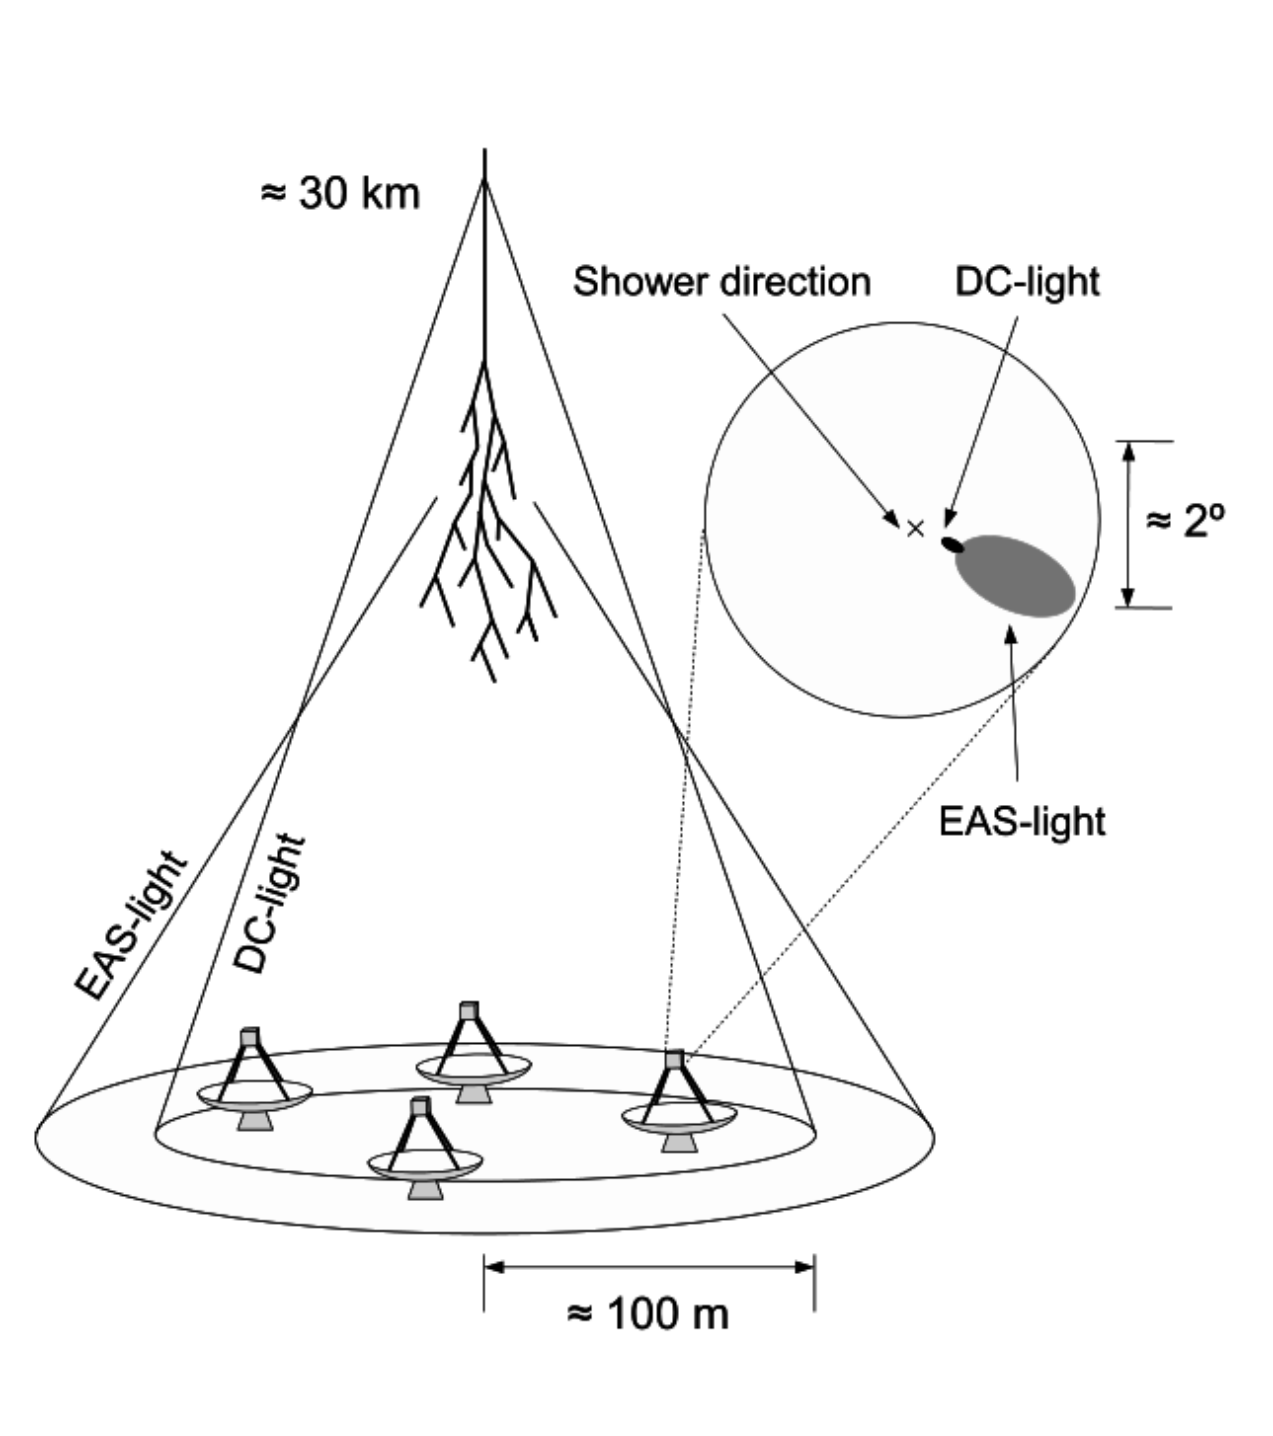
\includegraphics[height=0.3\textheight]{hessdiagram}
\caption{A diagram illustrating the HESS array \cite{hess07}. The four small telescopes are shown, but not the larger central telescope. The smaller Cherenkov ring is seen alongside the broader EAS light. A simplified camera image is also shown, and can be compared to a full image seen in Figure \ref{fig:fulltelimage}.}
\label{fig:hessdiagram}
\end{center}
\end{figure}

\section{DC Pixel Identification}
In a Comsic Ray event, the \textquoteleft Primary Particle' will emit Direct Cherenkov (DC) light in the upper atmosphere, before generating an Extended Air Shower (EAS) through interaction with the lower atmosphere. The primary particle is the Cosmic Ray itself, while the EAS refers to all daughter particle of the primary particle. In telescope images, the DC light is usually concentrated in a single  \textquoteleft DC pixel'. Identifying this pixel is challenging, because the brighter EAS Cherenkov light background often overlaps with the DC pixel. In order to apply the LPD method to data, we must first identify the DC pixel in a shower image, and determine the number of DC photoelectrons present. 

\subsection{Theoretical LPD}
To understand why DC light has a characteristic distribution, it is important to recall that Cherenkov emission begins when a charged particle passes the local speed of light in a medium.  We know that the refractive index of air is proportional to the density of air. Thus, the minimum velocity needed for Cherenkov Emission is lower for low atmospheric altitudes, because the air is denser. If the velocity is sufficient, we will observe photon emission from the particle at the Cherenkov Angle $\theta_{c}$. We obviously require that the Cherenkov Angle is real, so then require $\cos(\theta_{c}) \leq 1$. The minimum required velocity $\beta_{min}$ is thus equal to the inverse of the local refractive index $\eta$. 

\[ \cos(\theta_{c}) = \frac{1}{\eta \beta}  \Longrightarrow \beta \geq \frac{1}{\eta}\]

The velocity of a particle is a function of its energy, determined with the relations $\gamma = \frac{E}{m_{0} c^{2}}$ and $\beta^{2} = 1 - \frac{1}{\gamma ^{2}}$. Thus, we find that the minimum velocity ultimately leads to an Energy per unit mass threshold. If we assume that the slight difference in proton and neutron mass is negligible here, than any atmospheric altitude will have a local Energy per Nucleon threshold, and this threshold will be the same for all Cosmic Rays. 

The Energy per Nucleon Threshold for Cherenkov Light Emission as a function of height is illustrated in Figure \ref{fig:generalenergy}. Once the Energy of a Cosmic Ray exceeds the local Cherenkov Energy Threshold of the atmosphere, the Nucleus will begin emitting a ring of Cherenkov Light.  Then, for a given Telescope Array altitude above sea level and a given height h, simple trigonometry yields the final radius of emission on the ground:
\[ Radius(h) = \tan (\theta_{C}(h)) \times (h - altitude_{array})\]

The refractive index as a function of height is shown in Figure \ref{fig:lpd}, using standard values listed in the appendix. Because the refractive index of air increases very quickly as the height decreases, the Cherenkov Angle $\theta_{C}$ will also increase rapidly with decreasing height. Thus, although the displacement $(h - altitude_{array})$ decreases with height, the radius on the ground will nonetheless increase as height decreases. Consequently the upper atmosphere emission contributes to the inner LPD, while the lower atmosphere emission contributes to the outer LPD. As the cosmic ray travels down through the atmosphere, Cherenkov Emission continuously illuminates new areas on the ground that were previously unlit, without re-illuminating inner regions. 

Emission continues until the first interaction with the atmosphere, occurring at a randomly distributed height we call $h_{int}$. The maximum radius of the DC light will then be $r_{max} = Radius(h_{int})$. This is extremely useful, because for all distances up to $r_{max}$, the LPD will be completely independent of the interaction height. One full parameterisation of the LPD will thus be valid for all heights, provided the maximum radius is known.

Above threshold, Cherenkov Emission is determined by the Frank Tamm formula \cite{ppreview}.  Under the assumption of constant magnetic permittivity and a zenith angle of $90^{\circ}$, and with  the vertical distance travelled in meters $\Delta_{h}$ and the emission energy range in eV $\Delta_{E}$, we can find an approximate Cherenkov Emission formula.
\[ \frac{d^{2}N_{photons}}{dEdh} = \frac{\alpha Z^{2}}{\hbar c} \sin^{2} \theta_{c}(E) \approx 370 Z^{2} \sin^{2} \theta_{c}(E)\, cm^{-1}eV^{-1} \]

\[ N_{photons} \approx (37000 \times Z^{2} \times \Delta_{h} \times \Delta_{E}(E))\, m^{-1}eV^{-1}\]
 
A full simulation of the LPD was undertaken, with the assumption that $\Delta_{E} \approx 0.7 eV$ independent of Energy. Although this is certainly an oversimplification of the true picture, it will allow us to understand the variation of the LPD with height. A more rigorous LPD parameterisation will be found later to account for the dependence of $\Delta_{E}$ on the Energy. 

If we divide the number of emitted photons by the area of the annulus between the ring radii at $h$ and $h - \Delta_{h}$, we retrieve the LPD shown in Figure \ref{fig:lpd}, which varies with $ \rho_{DC}  = f(r) \times Z^{2}$. Thus the amplitude of the LPD is proportional to the square of the Cosmic Ray charge, enabling us to reconstruct this number from the DC emission. This proportionality is the basis for charge reconstruction in the LPD method.

\begin{figure}
\begin{center}
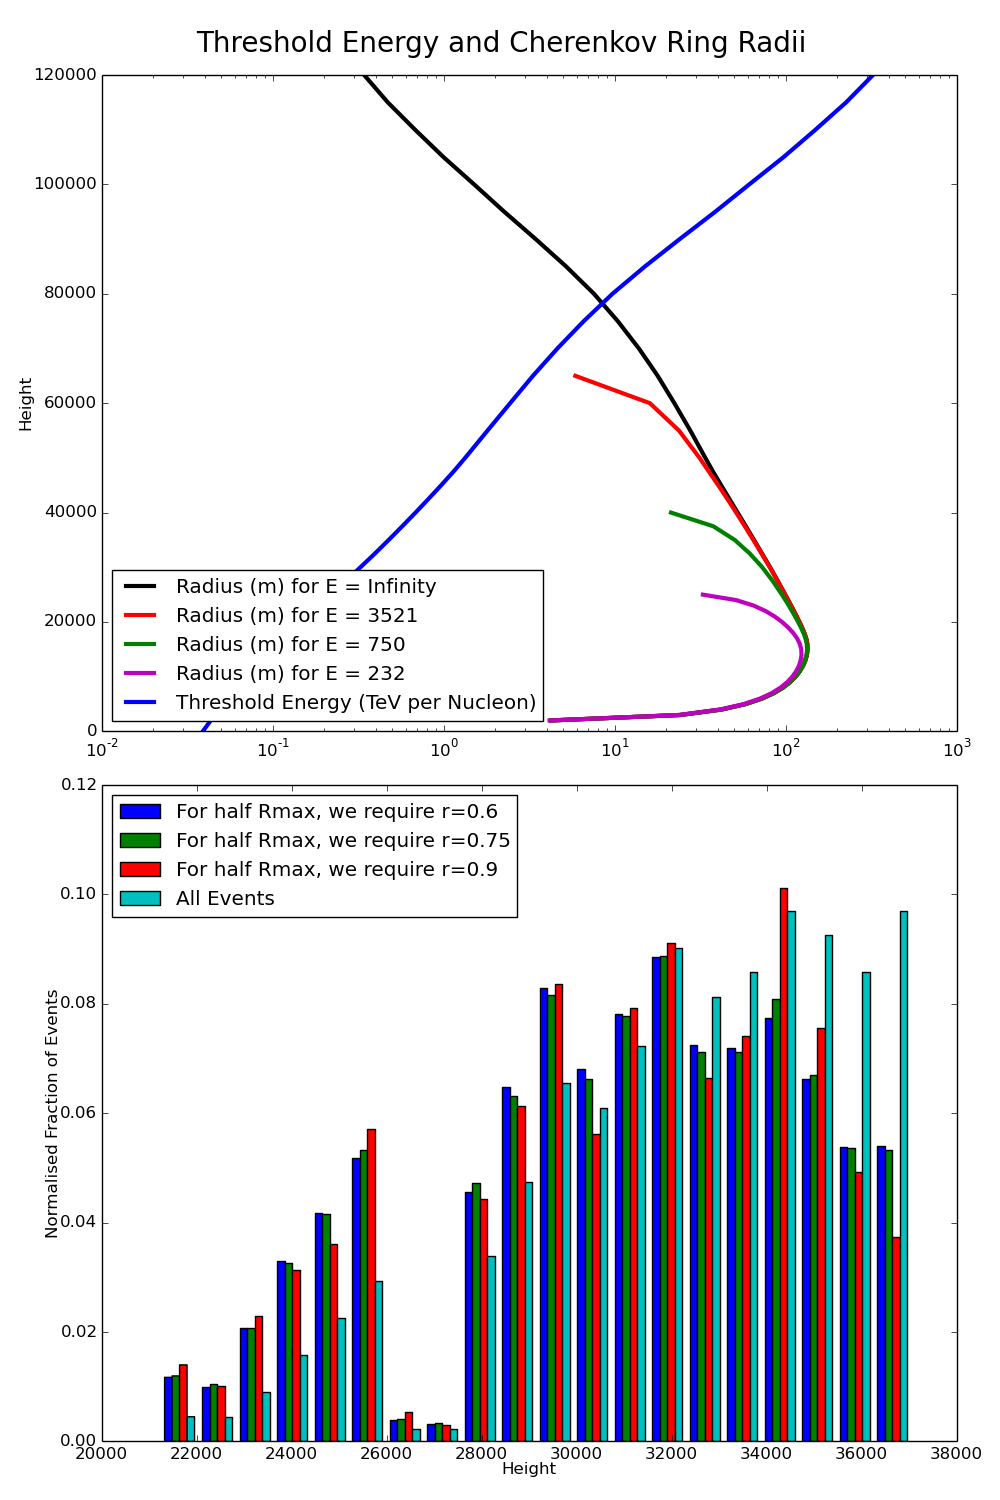
\includegraphics[height=0.9\textheight]{logenergyradius}
\caption{The Threshold Energy for Cherenkov Emission is marked in blue. With the assumption of $\beta=1$, the maximum emission radius is marked in black. The red and green and magenta line show the emission radius at 3.57 and 0.75 and 0.23 TeV per Nucleon respectively. The Green 0.7 TeV line is sufficiently close to the background to be saturated at 24km, while the magenta line is not.}
\label{fig:generalenergy}
\end{center}
\end{figure}

\begin{figure}
\begin{center}
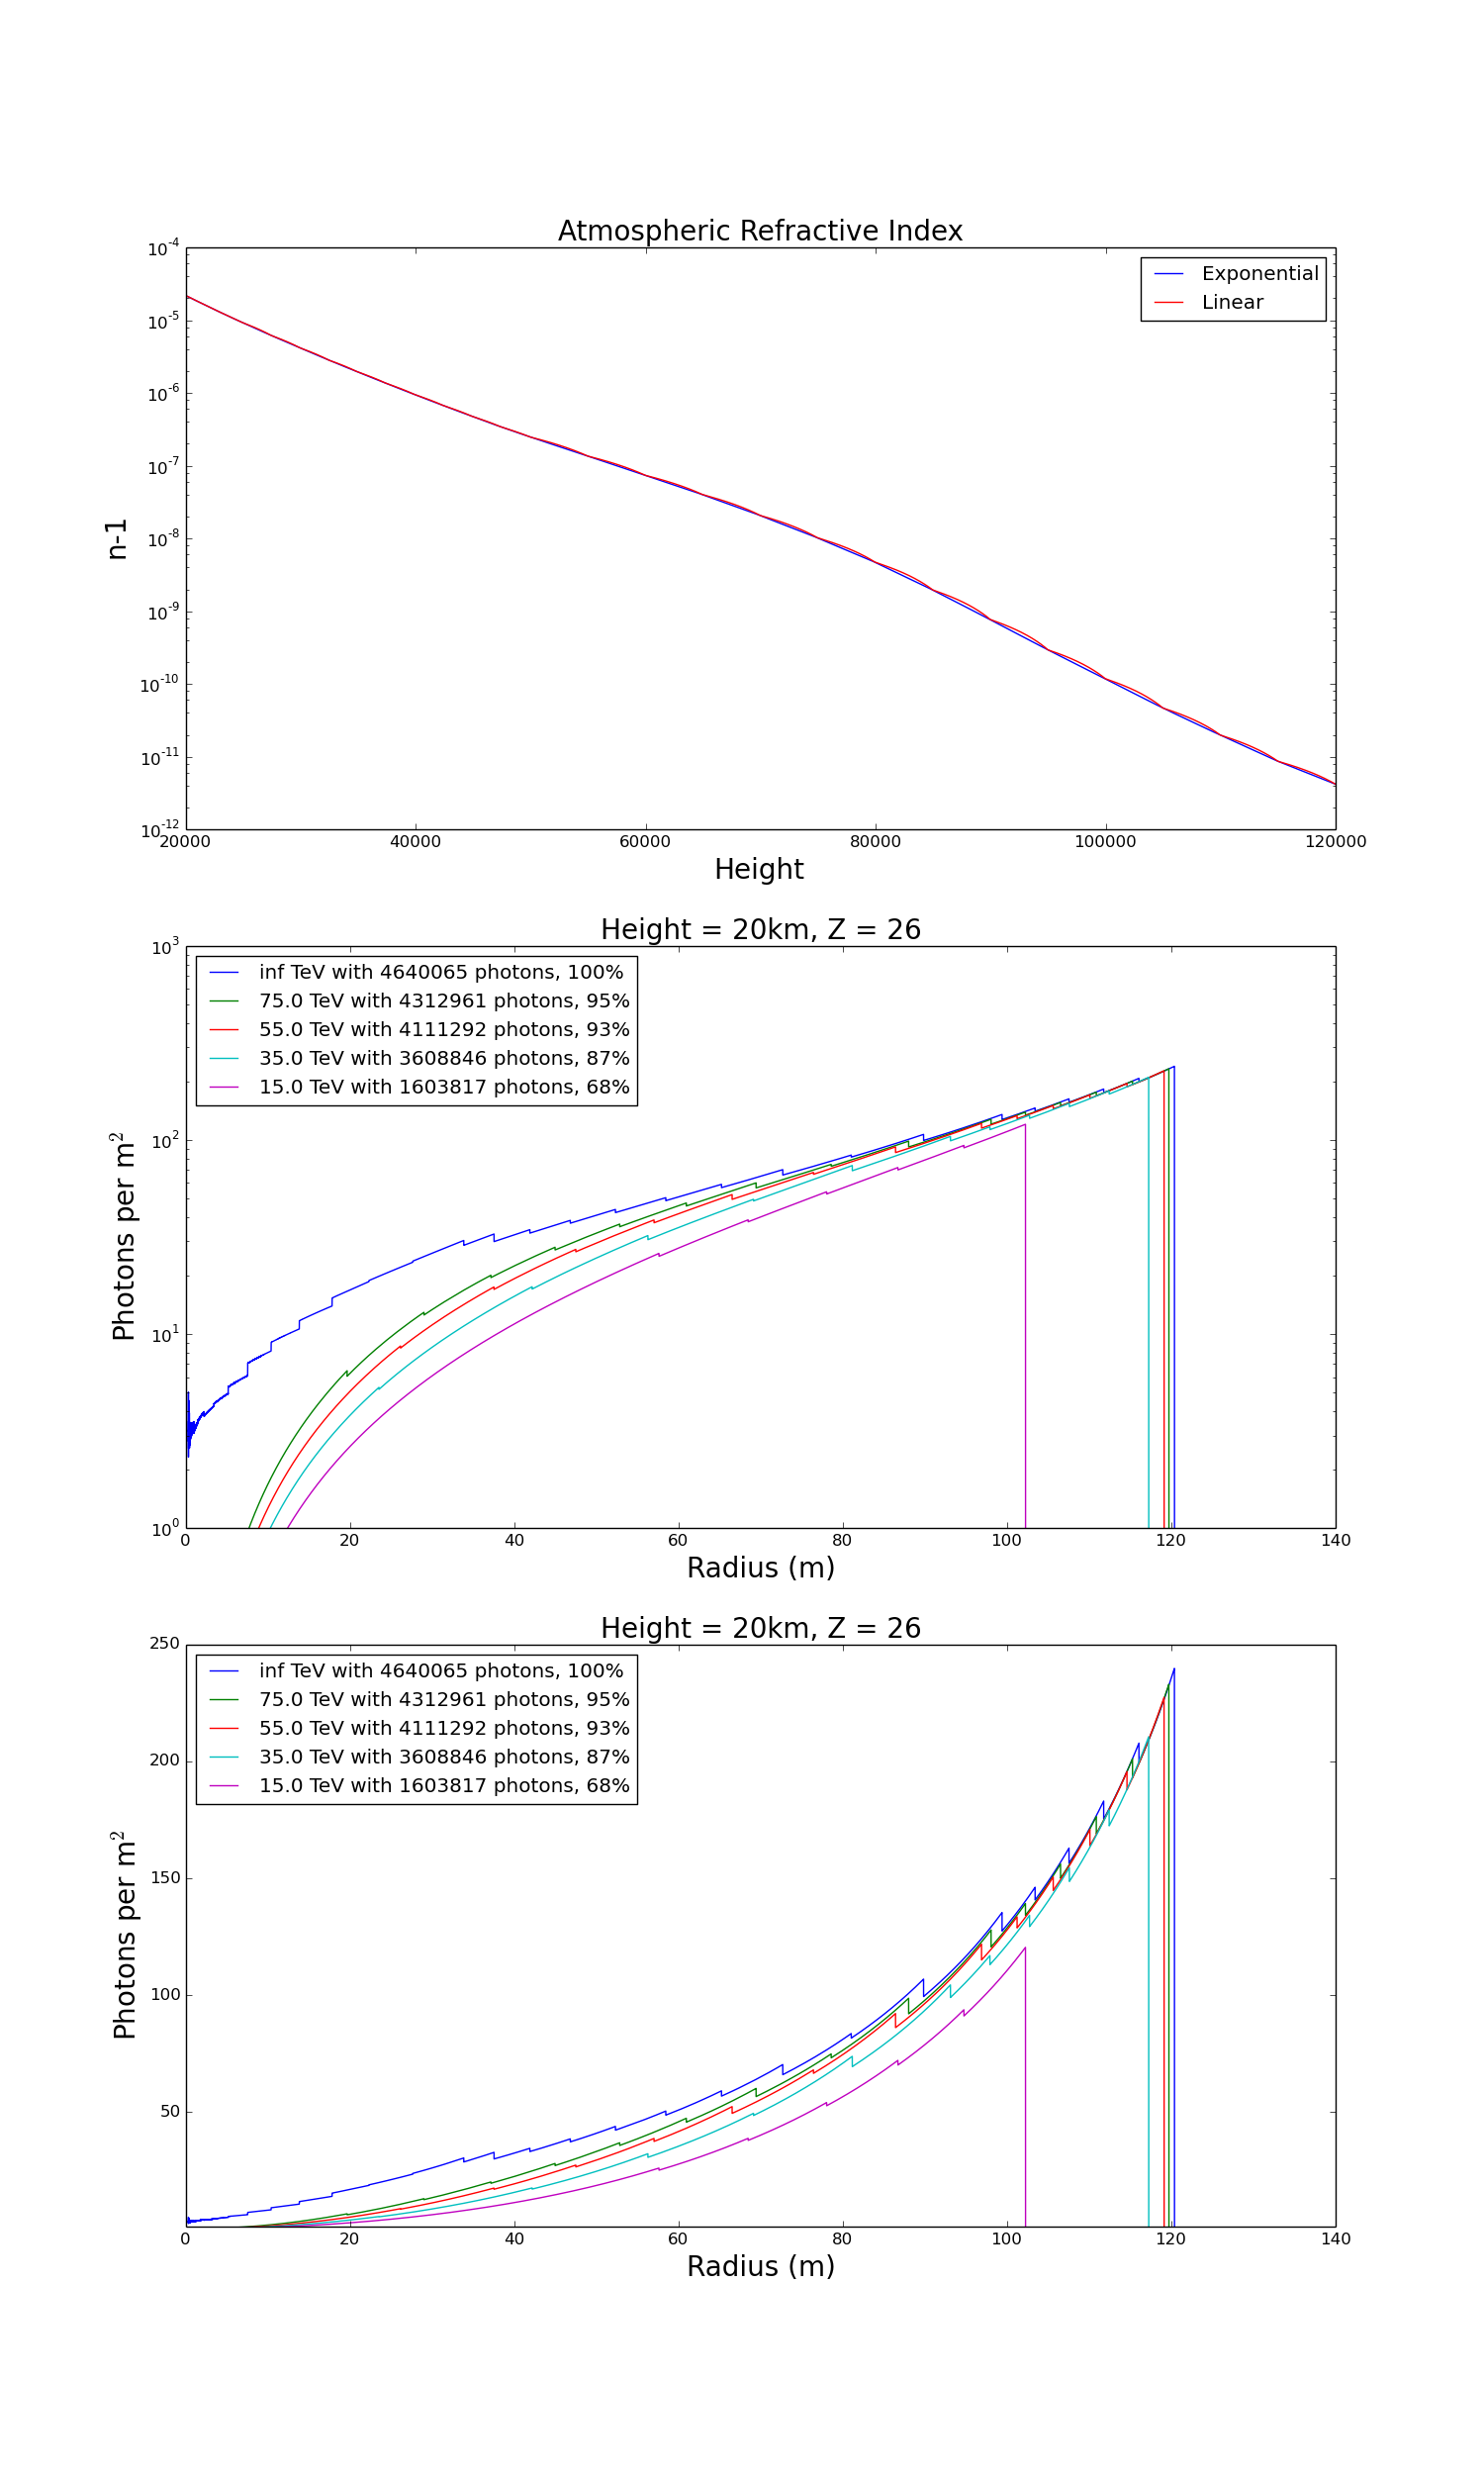
\includegraphics[height=0.9\textheight]{simulatedlpd}
\caption{Above, the refractive index is shown with both linear and exponential interpolation between the known values. The LPD obtained from simulation of an Iron Nucleus up to a first interaction height of 20km for a range of Core Energies. An altitude of 1.8km for the experimental array is assumed. Atmospheric absorption, although neglected, is broadly constant across the emission range leading to uniform amplitude scaling.}
\label{fig:lpd}
\end{center}
\end{figure}

The refractive index at a series of heights, based on data from the HESS site, is also shown \ref{fig:lpd}. Exponentials are fitted between points to provide interpolation, and a comparison can be made to a linear interpolation that is also plotted. Despite the exponential interpolation, discontinuities in the second derivative of the refractive index prevent the LPD from being smooth in the simulation. This is unimportant, because in reality the variation due to atmospheric conditions and random noise will smear out any discontinuities in the LPD.

We can also see ground emission radius as a function of height in Figure \ref{fig:generalenergy}. We find that the high-radius emission (occurring near the first interaction region) varies little between different high energies. We deem this to be \textquoteleft Saturated Emission\textquoteright. To accurately quantify Saturated Emission, we can compare the photon density to the theoretical maximum photon density, corresponding to an infinite-energy particle with $\beta =1$ in Figure \ref{fig:lpd}. The illustrated maximum is useful as a reference, although because the atmosphere is not modelled beyond an altitude of 120km, the small-radius emission is not accurately simulated entirely correctly. However, real cosmic rays in the considered energy regime will all cross the emission threshold and begin emission at an altitude much lower than 120km, so can be considered accurately modelled.

For energies above 25 TeV, we see that there is a clear characteristic photon distribution which is almost independent of Energy except for a varying endpoint. The LPD displays many discontinuities, which can be explained by the interpolation of Refractive Index. Exponential Interpolation will not provide a function that is smooth for second or third derivatives, and consequently, the LPD is not smooth. In reality, there will be a funtion describing the Refractive Index as a function of height, but it will depend on many variables such as Temperature. This will be the dominant cause of variations to the LPD, and thus, uncertainty in the LPD from Refractive Index Interpolation will be sub-dominant.

In any case, we will not be able to directly measure this LPD. Instead, a telescope images containing air showers must be analysed, and from these images, we can infer the quantity of DC light present amongst a large degree of background. Extensive simulations of Camera images will be performed, in order to quantify the resultant LPD extracted from the telescope images. After determining a likely experimental LPD, Monte Carlo events can be simulated, and then reconstructed. 

\subsection{Image Simulation}
The CORSIKA package \cite{Heck98} was used to generate Cosmic Ray events, and the Sim\textunderscore telarray package  \cite{Bernlohr08} was used to generate corresponding HESS array telescope images.  Simulation with EAS background was used to produce training pixel sets, while corresponding simulation without EAS background was used to find the true DC pixel in each training image.

The full simulation of air showers was performed using CORSIKA with a standard atmospheric profile derived from measurements conducted at the HESS site in Namibia. This is included in the Appendix. In total, 5000 training events and a further 10000 testing events were simulated. The simulated particles were $Fe^{56}$, within the Energy Range of $35-135$ TeV and a flux spectrum $\phi(E) \propto E^{-2.7}$. For each set of simulated event, 4 unique random number seeds were used to generate the shower. An altitude of 1800m was assumed, again corresponding to the HESS site. The simulated zenith angle ranged from $0^{\circ} < \theta < 2 ^{\circ}$, while the simulated azimuth angle ranges from $-2^{\circ} < \phi < 2 ^{\circ}$. The four smaller HESS-phase-1 telescopes were arranged in a cross along the x/y axis with the larger HESS-phase-2 \textquoteleft CT5' telescope placed at the center. The length of each cross arm was $85m$. The simulated target region of the cores was chosen to be a square centered on CT5, with each 300m-long side bisecting the x/y axis. Due to hardware differences between CT5 and the original HESS 1 telescopes, we analyse HESS1 and HESS2 images separately. 

To determine the true class of each pixel, a simulation was initially run with an energy cut of 10 PeV on all muons and electrons. Because this cut exceeded the primary particle energy, neither daughter muons and electrons, nor the photons they would have emitted, were simulated. Thus the hadronic Cherenkov Light from the primary particle and daughter fragments, but not the EAS light, was present in the camera image. A second identical \textquoteleft EAS Simulation' was run including the same random seeds, but without the energy cut on muons and electrons. This gave a complete EAS image including identical DC light. The difference is well-illustrated in Figures \ref{fig:DCtelimage} and \ref{fig:fulltelimage}.

With the sim\textunderscore telarray package, the expected HESS hardware response to each air shower was simulated. Among other things, the program accounts for atmospheric transmission and density, mirror positions, sizes and reflectivities, camera shadowing and triggering, quantum efficiency and pulse responses. For the full-shower image, the night sky background was also simulated by sim\textunderscore telarray. Due to the comprehensive and detailed nature of these hardware simulations, the resultant images can be considered \textquoteleft realistic'.  However, sim\textunderscore telarray introduces various sources of random noise to the simulation, leading to some divergence in the DC light between the EAS-free and full-shower images.

\begin{figure}
\newgeometry{a4paper, portrait, margin=1.0in}
\centering
\begin{minipage}{0.45\textwidth}
\centering
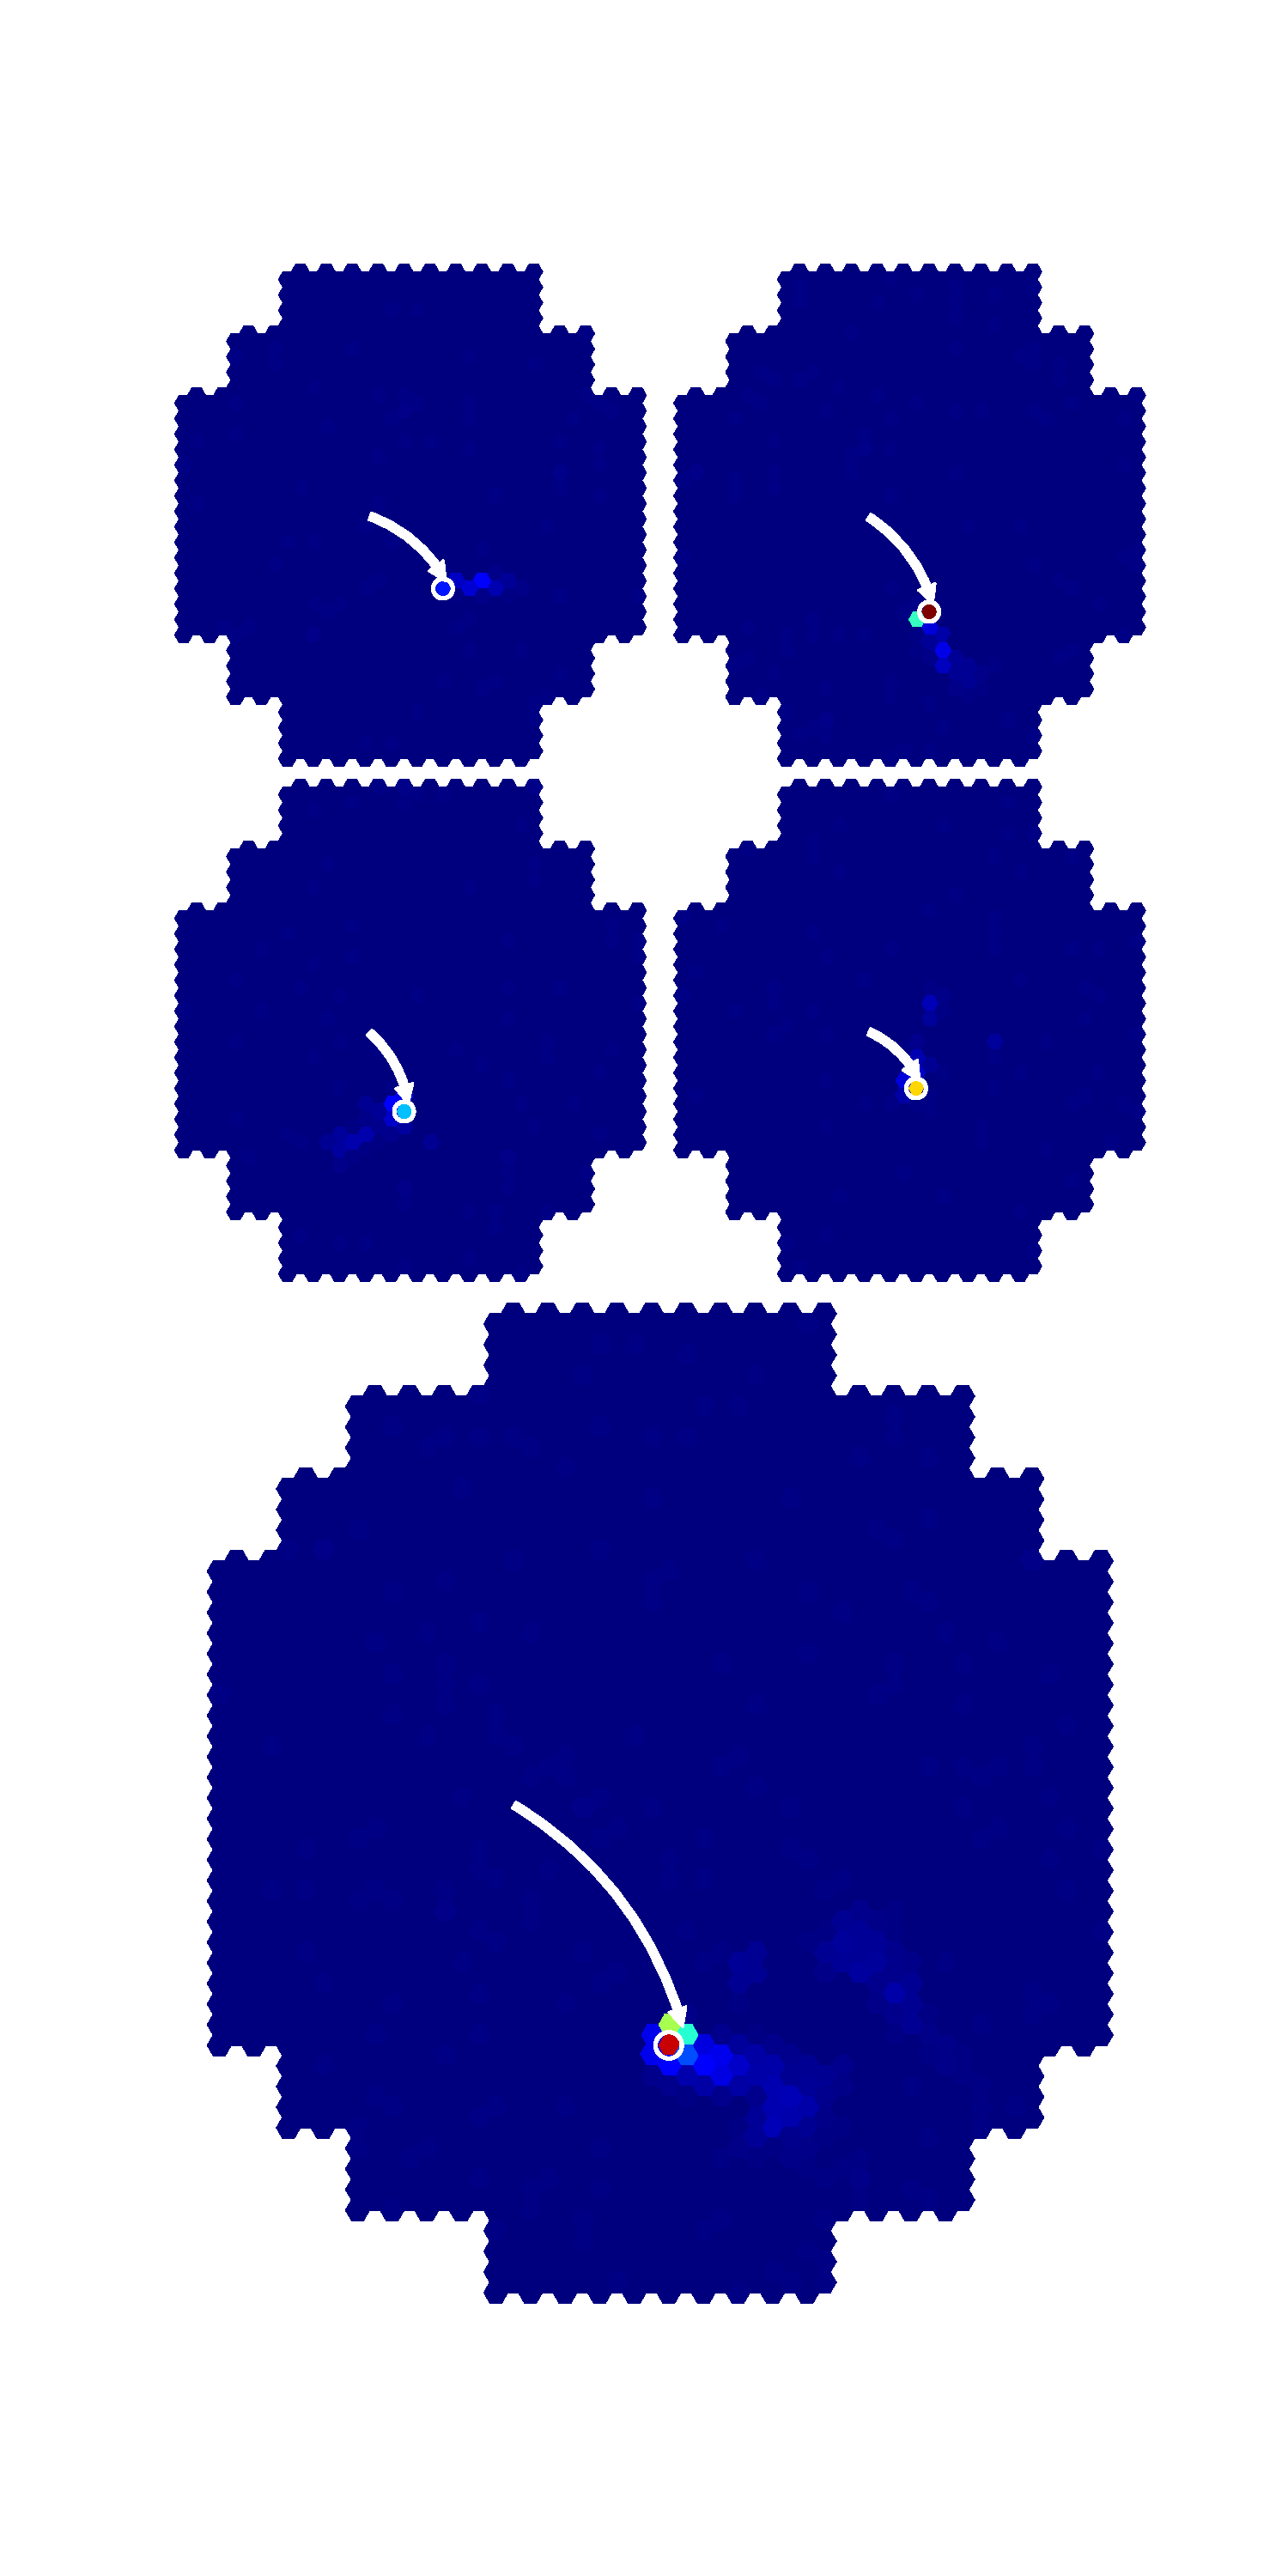
\includegraphics[trim=80 120 80 150,clip,width=\textwidth]{graphDC}
\caption{An ideal camera image without the EAS shower. The DC light is visible in every telescope, indicated by the white arrow. The DC pixel is circled in white. The largest telescope image is from CT5, and is analysed separately.}
\label{fig:DCtelimage}
\end{minipage}\hfill
\begin{minipage}{0.45\textwidth}
\centering
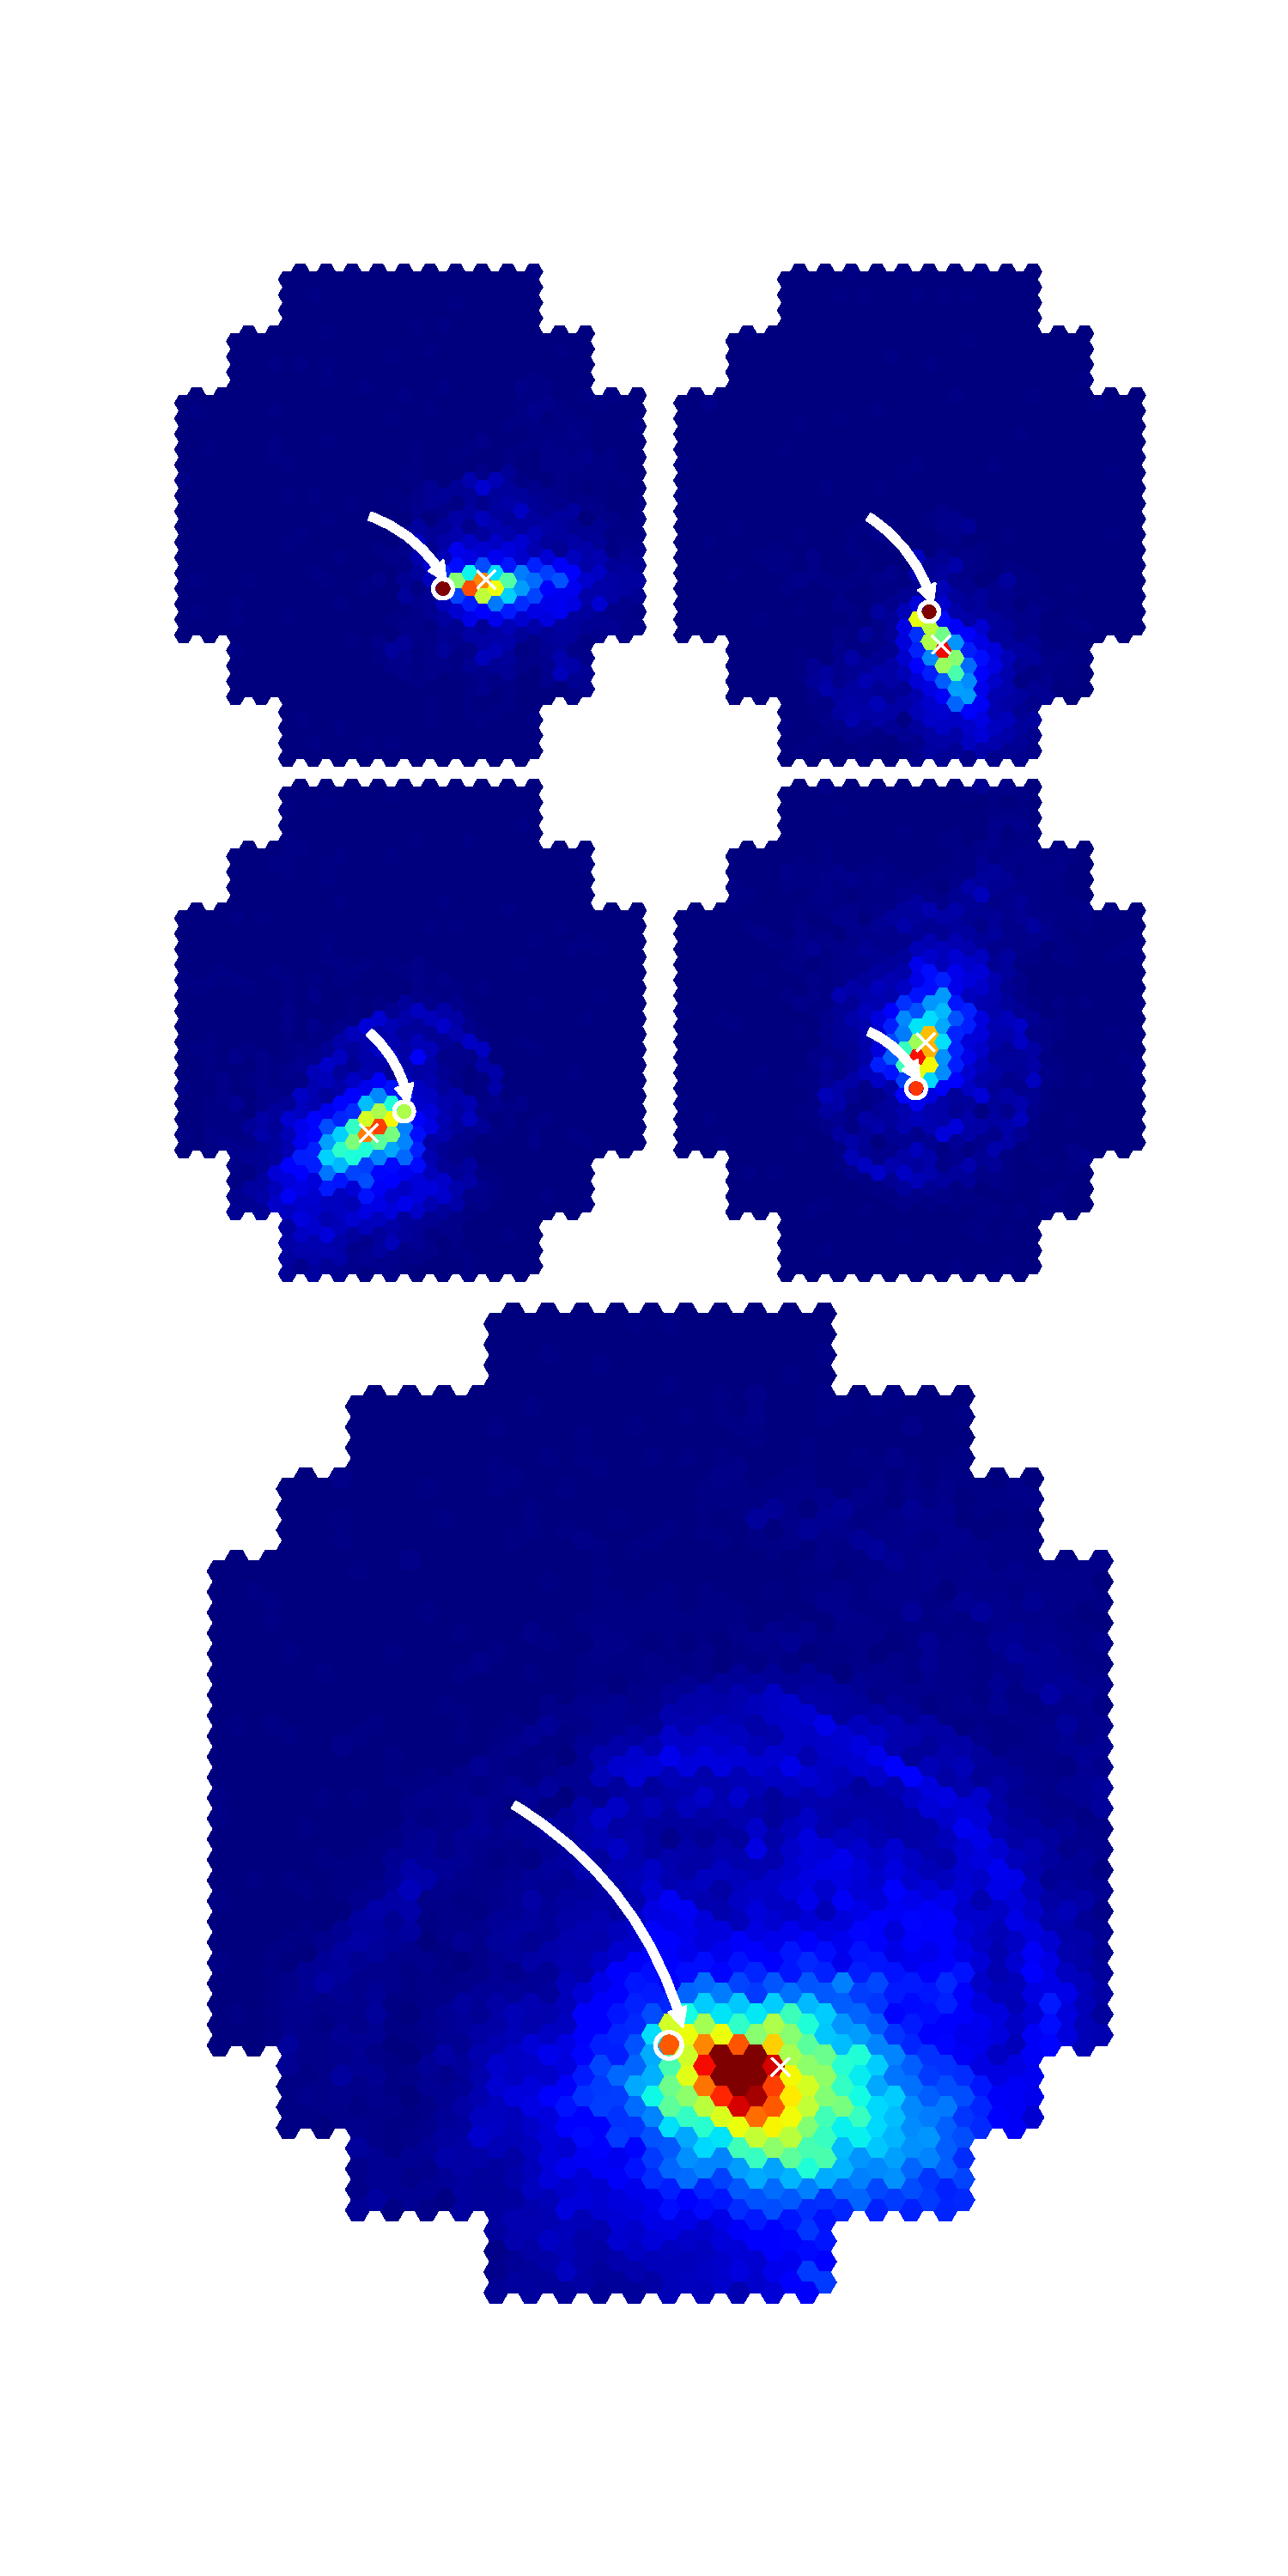
\includegraphics[trim=80 120 80 150,clip,width=\textwidth]{graphfull}
\caption{This is a typical camera image. The same shower as in Figure \ref{fig:DCtelimage} is shown here with the inclusion of the EAS shower.  The DC light is pixels indicated with a white arrow and circle. The shower center of gravity is marked by a white cross.}
\label{fig:fulltelimage}
\end{minipage}
\restoregeometry
\end{figure}

The various pixel entry variables were found from the sim\textunderscore telarray output. The HESS telescope pixels have a high gain Channel 0 and a low gain Channel 1, with both voltages undergoing a Flash Analogue-to-Digital Conversion (FADC). The simulated value of the FADC Voltage for each channel was found. Using the pedestal and gain, the quantity $Intensity = (FADC - Pedestal)\times Gain $ was calculated for each channel. Due to possible saturation of the high gain FADC, only the low gain $Intensity$ was used. Sim\textunderscore telarray also derives various Hillas whole-image parameters. These include the image width and length measured in degrees, from which the aspect ratio $A.R = \frac{width}{length}$ was calculated. The reconstructed shower direction and the shower center of gravity were also calculated, as positions in azimuth and zenith. Additionally the estimated energy and distance from each telescope to core, $r_{core}$,  were found.

For every pixel, in addition to the $Intensity$, its location within the telescope image was determined using the standard HESS layout. The variables $ \Delta_{C.o.G}$, $\Delta_{Direction}$ and $\Delta_{Line}$ were defined as the distance from the pixel to the shower center of gravity, shower direction, and the line joining those two points. Furthermore, the nearest neigbouring pixel IDs were calculated for every pixel position, enabling the $Intensity$ in each neighbouring pixel to be found. The largest neighbouring intensity was identified, and the ratio $Q_{DC} = \frac{Intensity_{N.N.max}}{Intensity}$ was derived. Similarly the largest neighbouring FADC was found, and the ratio $raw_{Q} = \frac{FADC_{N.N.max}}{FADC}$ was calculated. In addition, the Nearest Neighbour Mean Intensity $Mean_{N.N}$ was recorded, as well as the smallest neighbouring pixel intensity $Intensity_{N.N.min}$. The variable $DC_{Signal} = Intensity-Mean_{N.N}$ was defined as an rough guess of the \textquoteleft DC signal' component in the pixel. Lastly the Image Amplitude $I_{tot}$, defined as the total image intensity after the default tail cuts have been applied to the image.

\subsection{Classic HESS1 DC Pixel Identification}
We can find the DC pixel in an image with the variable $Q_{DC}$. In previous experiments, the DC pixel candidate was identified by applying a number of cuts to pixels in an image \cite{hess07}, and from the subset of pixels passing the specified cuts, selecting the pixel with the smallest $Q_{DC}$ as the \textquoteleft DC candidate'. Due to the low pass rate for cuts, we obtain a small low-contamination dataset, while the majority of telescope images are left without a DC pixel candidate. 

As a basis for comparison, these original HESS cuts listed in Table \ref{tab:qdccuts} were replicated for the set of test data. For every HESS1 image, the total image amplitude $I_{tot}$ was used alongside the zenith angle $\theta$ to determine a dynamic cut, $Q_{DC} < 0.14 \times \log(\frac{I_{tot}}{161 \times \cos \theta})$. Because many images had no pixel that passed all cuts, the $Q_{DC}$ method was frequently unable to identify a DC pixel. In the original analysis, an additional cut $r_{core} \textgreater 40m$ was applied. However, the uncertainty in determining the core position through Hillas Analysis is typically of the order of $\pm 20m$. Consequently, this particular cut was omitted, though it would only serve to further reduce the DC pixel acceptance rate.

\begin{table}[h!]
  \centering
  \caption{Cuts applied to image pixel sets, used by HESS collaboration \cite{hess07}}
  \label{tab:qdccuts}
  \begin{tabular}{ccc}
    \toprule
    Variable & Cut\\
    \midrule
     $ \Delta_{C.o.G}$ & \textgreater 0.17 \\
     $ \Delta_{C.o.G}$ & \textless 0.91 \\
     $\Delta_{Direction}$ & \textless 0.45 \\
     $\Delta_{Line}$ & \textless 0.23 \\
     Aspect Ratio & \textless 0.75 \\
     $Q_{DC}$ & \textless 0.14$ \times \log(\frac{I_{tot}}{161 \times \cos \theta})$ \\
    \bottomrule
  \end{tabular}
\end{table}

The candidates were checked against the true DC pixels identified in the EAS-free images. From the testing sample, 1.81\% of all HESS1 images were correctly identified and passed the cuts. Once misidentified events were considered, the post-cuts sample was 77.8\% accurate, as shown in Figure \ref{fig:cutdistribution}. These values will serve as a useful benchmark for BDT performance. Increasing the acceptance rate will be essential for enabling spectroscopic analysis of cosmic rays, by providing more events to analyse. An improved method would aim to increase the number of correctly identified DC pixels, while still enabling cuts which discriminate well between correctly and incorrectly identified DC pixels.

\begin{figure}
\begin{center}
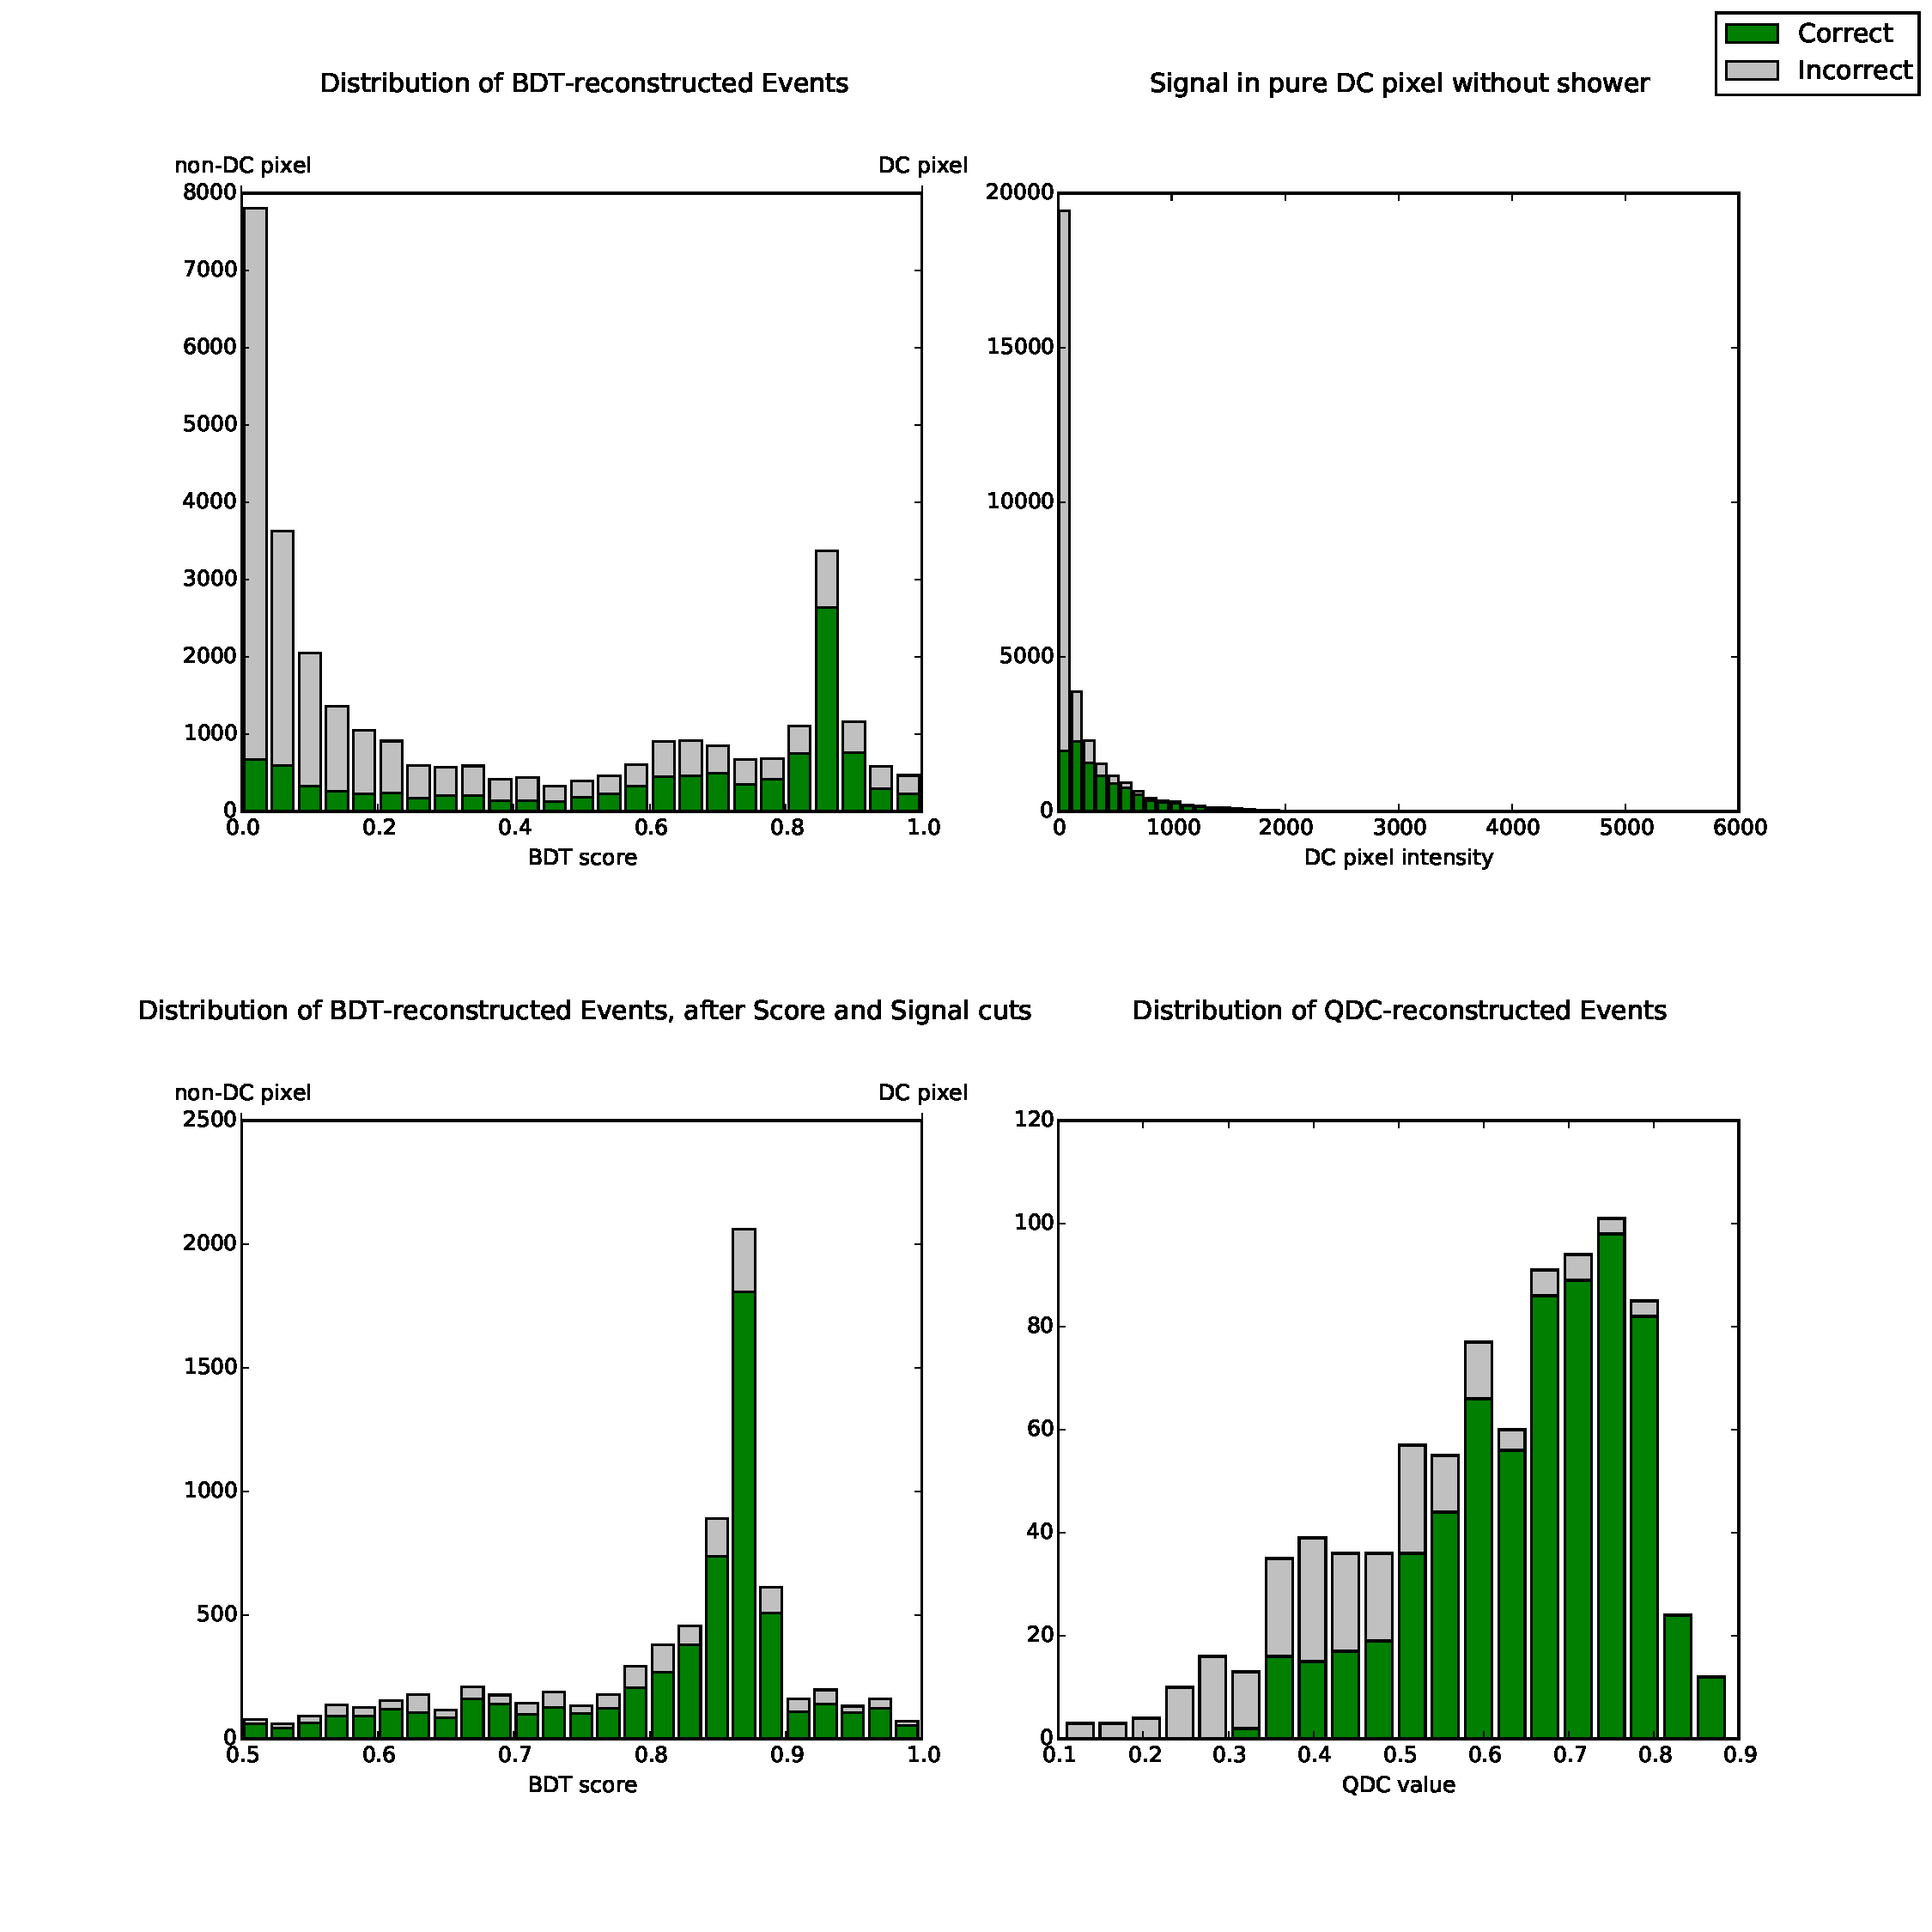
\includegraphics[width=\textwidth]{hess1statsbigtestdata}
\caption{The DC signal in the shower-free pixel is shown in the top right, following an exponential decay. Events below roughly 200 are unlikely to be identified correctly because the DC light is too faint to be seen against the background. In the top left, the BDT score distribution is shown before any cuts. In the lower left, we see the same distribution after both signal and BDT score cuts are applied. For comparison, the lower right graph shows the alternative distribution of $Q_{DC}$-reconstructed events. All green events are ones in which the DC pixel has been correctly identified, while grey events are ones that have been incorrectly identified.}
\label{fig:cutdistribution}
\end{center}
\end{figure}

\subsection{Boosted Decision Tree DC Identification}
Classifiers provide an alternative method of DC pixel identification, making use of supervised machine learning to find rules for categorising pixels. To train a classifier, we require a set of training pixels, as well as the correct class for each pixel. Once trained, a classifier can then be used to predict the class of a pixel. As part of a new method developed for this analysis, a Boosted Decision Tree (BDT) classifier was trained to identify DC pixels using the Scikit Learn Python package \cite{scikit-learn}.

A Decision Tree is a simple method of classification, in which a number of branching decisions are used to place events into one of many \textquoteleft leaves'. A leaf lies at the end of every decision chain, and will be associated with one of the possible classes. Any event being assigned to a particular leaf will then be classified as belonging to that leaf's class. Each branch and leaf has a sample, which indicates the number of training events that are placed in there. As part of the machine learning process, branches are constructed to maximise leaf purity. A hypothetical perfect branch would split a mixed sample into two pure leaves. 

It will almost always be possible to construct a tree, such that each event was placed in its own, unique leaf. The performance of a tree would be perfect for the training set. However, if applied to a separate testing sample, the performance would be significantly worse. The tree would not be classifying data, but rather simply remembering the structure of the training data. We describe such a tree as being overtrained.

In general, larger training sets prevent overtraining by making it more difficult to uniquely distinguish the individual events. The maximum depth of a tree is the number of branches a decision chain can pass through before it must end on a leaf. The minimum leaf sample is the minimum number that every leaf sample must exceed. Either of these quantities can also be used to restrict overtraining of a Decision Tree.

A graphical representation of a Decision Tree is given in Figure \ref{fig:decisiontree}. Decision Tree training is highly unpredictable, meaning similar datasets can produce wildly differing trees. Thus Boosted Decision Trees are used to provide a more stable method of classification. The training of a Boosted Decision Tree is in some sense an averaging process, where many different Decision Trees are trained. One starting Decision Tree is produced, with each event having an equal weighting. After each iteration of tree production, any misidentified events in a tree are given a higher weighting for the training of the next tree \cite{Roe:2004na}. Over time, this leads to an improved learning process by focussing more on those events that are more difficult to classify.

\begin{figure}
\begin{center}
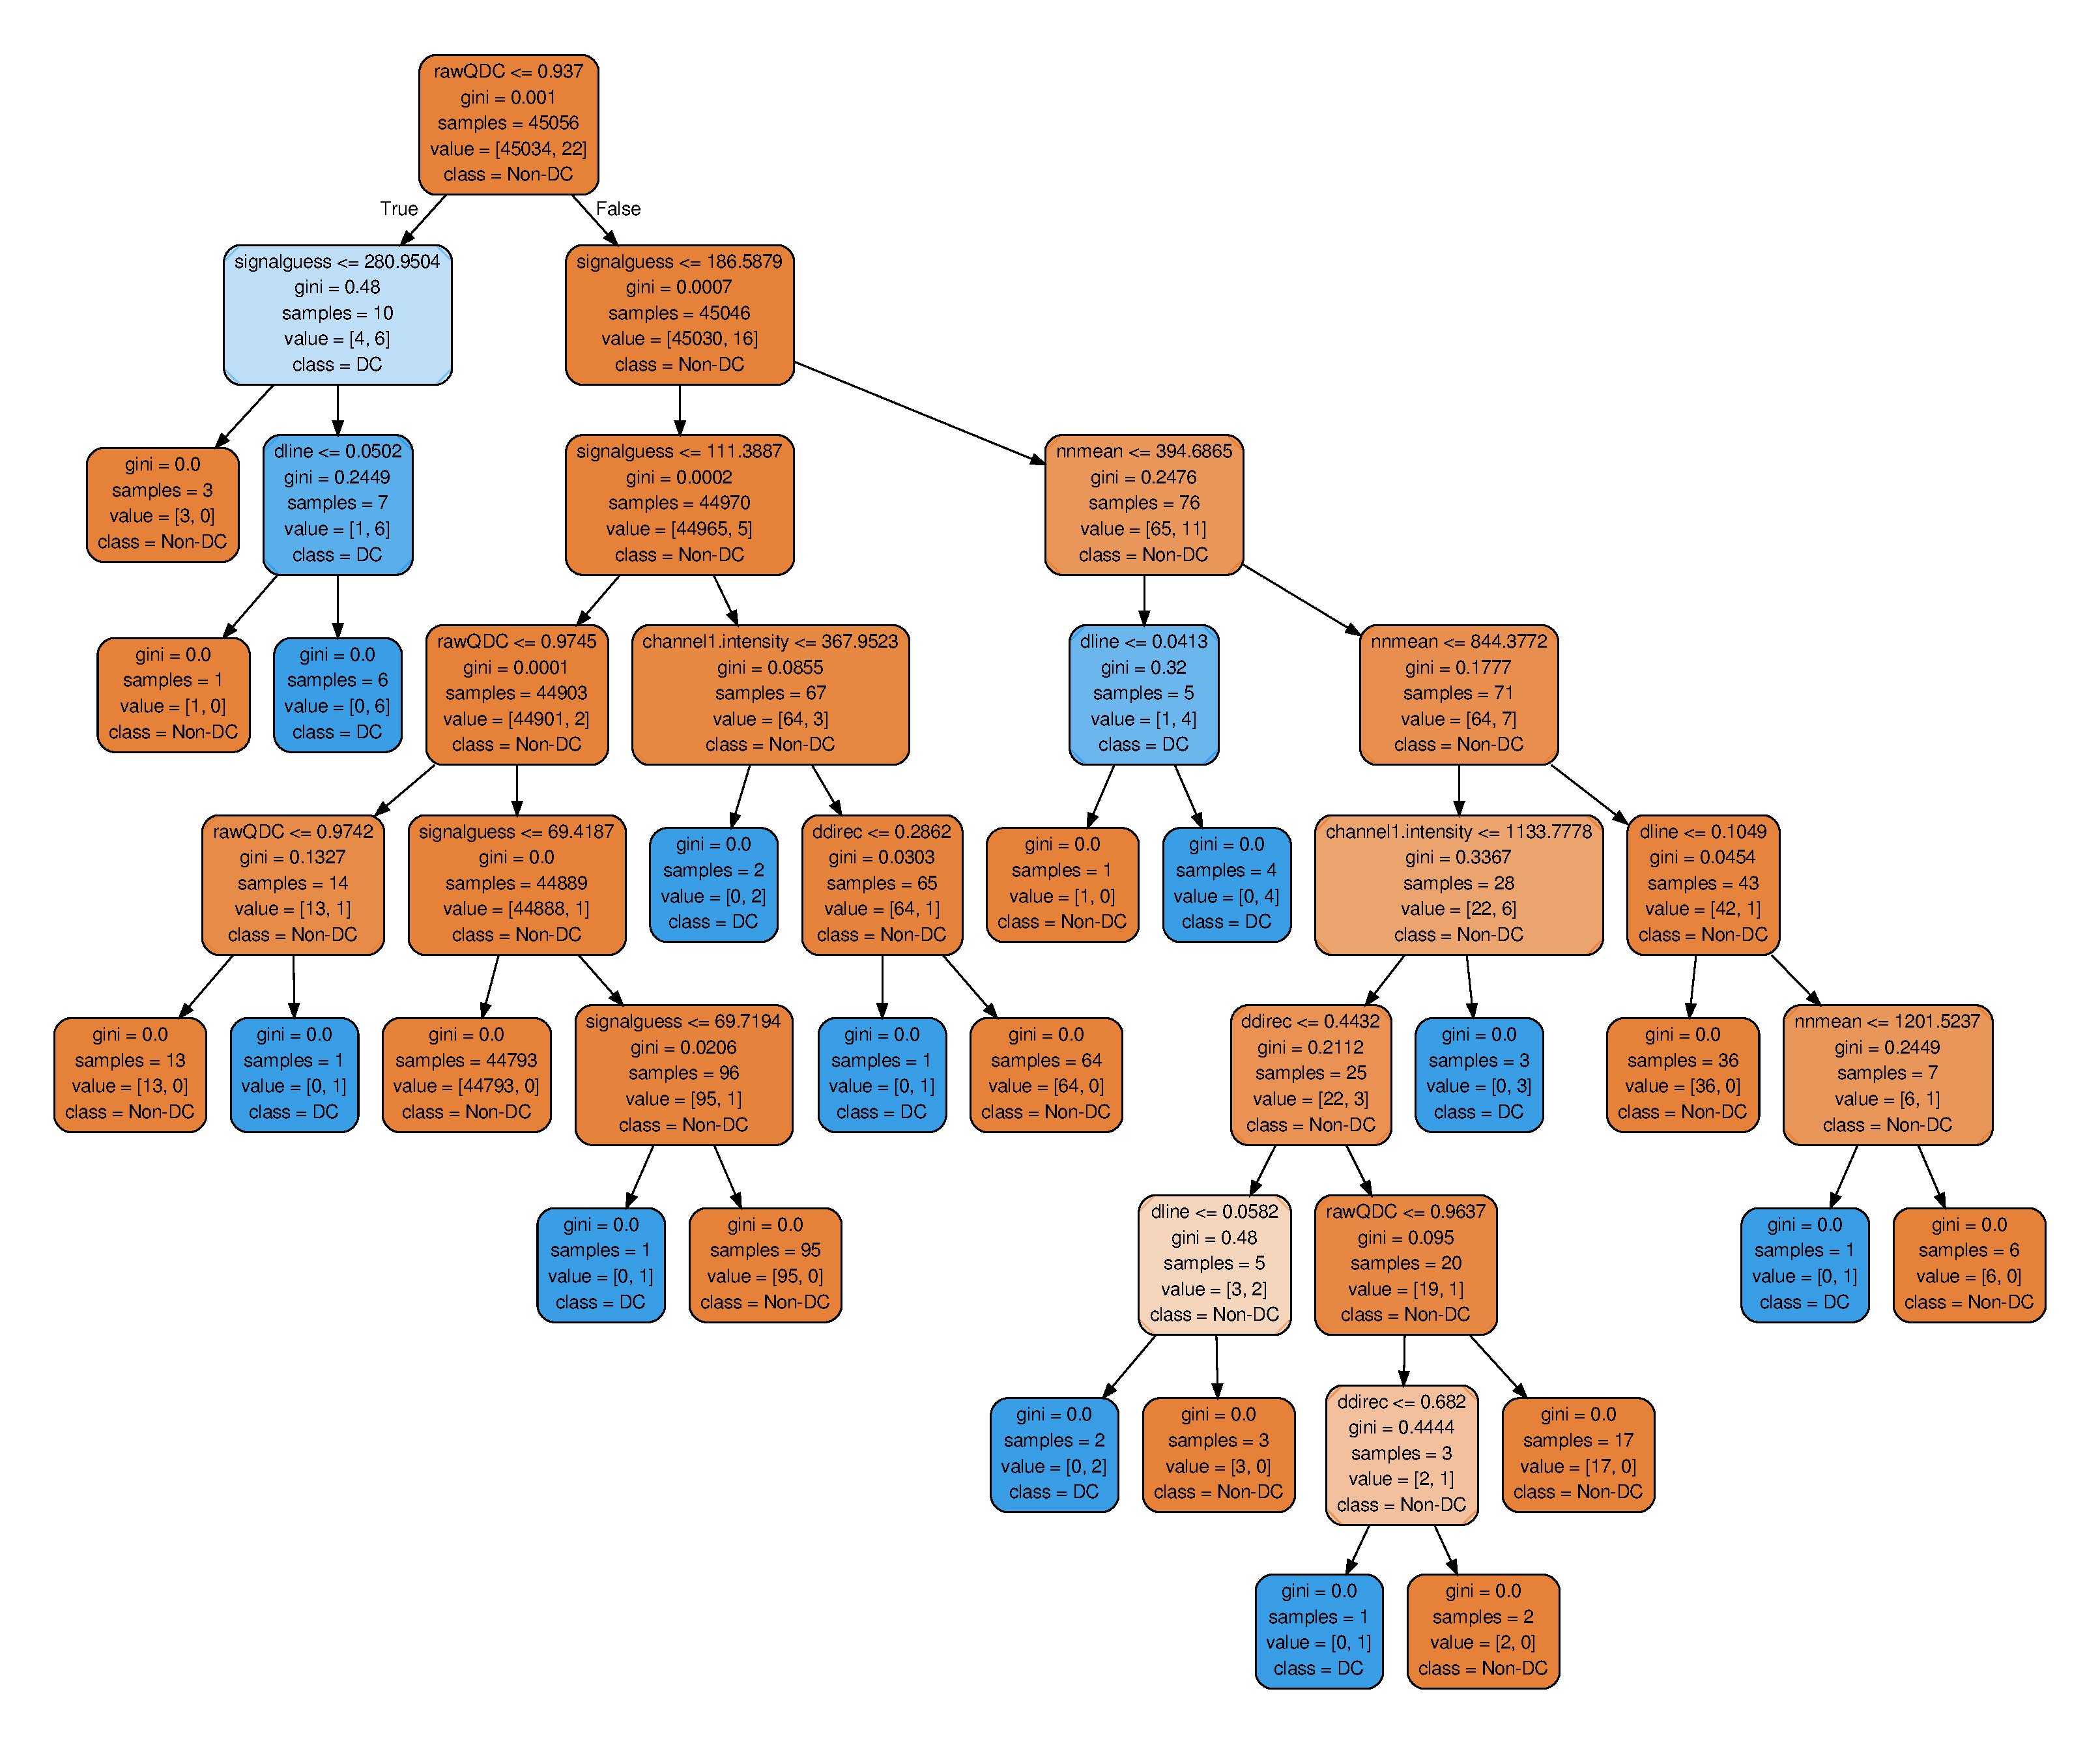
\includegraphics[width=\textwidth]{decisiontreehess1}
\caption{An example of a decision tree for the HESS 1 telescope system. The left direction is followed if the branch condition is true, while the right direction is followed if the condition is false. Red leaves contain non-DC pixels, while blue leaves represent DC pixels. The sample of each leaf is listed. Darker boxes have purer samples, while lighter boxes are more mixed.}
\label{fig:decisiontree}
\end{center}
\end{figure}

In this case, the training set consisted of pixels from 5000 CORSIKA events. It was randomly split further, with 90\% in a learning subset and 10\% in a subset to check for overtraining. Within the learning subset, every HESS 1 image was used, provided it was triggered in both EAS-free and full-shower simulations. For each of the triggered image pixels, an entry was formed with the variables listed in table \ref{tab:hess1classifier}. A class of 0 was assigned to every non-DC pixel, and a class of 1 was assigned to every DC pixel. Having created a dataset, the BDT was then trained with a maximum depth of 8, and with 1000 trees generated. The data was provided in the form of individual pixel entries, rather than as discrete sets for images or events.

\begin{table}[h!]
  \centering
  \caption{Relative Feature Importance in HESS-1 BDT training}
  \label{tab:hess1classifier}
  \begin{tabular}{ccc}
    \toprule
    Variable & Relative Importance\\
    \midrule
    $DC_{Signal}$ & 0.33\\
    $Mean_{N.N}$ & 0.24\\
    $Q_{DC}$ & 0.14\\
    $\Delta_{Direction}$ & 0.12\\
    Image Amplitude & 0.07\\
    $raw_{Q}$ & 0.05\\
    $\Delta_{Line}$ & 0.02\\
    $Intensity$ & 0.02\\
    \bottomrule
  \end{tabular}
\end{table}

The relative importance of each \textquoteleft feature' is automatically calculated by the Scikit Learn package, and is also recorded in table \ref{tab:hess1classifier}. The variable $DC_{Signal}$ was consistently the most importance variable across many combinations of included variables and BDT training parameters. It was found that, under the conditions listed above, the BDT was 99.94 \% accurate for the learning pixel subset, and 99.94 \%  accurate for the overtraining-check pixel subset. This indicates that the BDT was not significantly overtrained, which would otherwise be manifested by a large divergence in accuracy between learning and overtraining-check data.

Having trained the BDT successfully, it was then applied to the same test dataset as for the classic $Q_{DC}$ identification. In each camera image, the event with the largest BDT score was deemed to be \textquoteleft most signal-like', and thus selected as the DC pixel candidate. A cut was applied, requiring $P_{signal} > 0.5$ for the DC candidate to be accepted. A second cut requiring $DC_{Signal} > 150$ removed many incorrectly identified events. Application of this combined cut greatly increases the successful identification rate. From the testing sample, 16.01\% of all images were correctly identified and passed the cuts. The BDT was found to be 79.2\% accurate in identifying DC pixels which passed the cuts. This represents a very significant improvement in pixel identification efficiency, as well as a minor increase in accuracy after cuts. 

The results are summarised in Table \ref{tab:qdcbdtcomparison1}. The BDT method represents a clear improvement in DC pixel identification over the previous $Q_{DC}$ method, and corresponds to an eightfold increase in identified pixels. 

\begin{table}[h!]
  \centering
  \caption{Comparison of $Q_{DC}$ and HESS 1 BDT Performance}
  \label{tab:qdcbdtcomparison1}
  \begin{tabular}{ccc}
    \toprule
    & $Q_{DC}$ & BDT\\
    \midrule
    Accepted Pixels Correctly Identified (\%)  & 1.81 & 16.01\\
   Accepted Pixels Incorrectly Identified (\%)  & 0.52& 4.22\\
    Sample Purity (\%)  & 77.8 & 79.2 \\
    \bottomrule
  \end{tabular}
\end{table}

\subsection{HESS-2 BDT}
The original HESS study predated the construction of the larger CT5 telescope, and thus focused exclusively in the four HESS-1 telescopes. Although the cuts in Table \ref{tab:qdccuts} were not optimised for the differing pixel size and angular viewing region of CT5, they were replicated to provide a basis for comparison. Based on CT5 images from the training sample, an increased 5.6\% of DC pixels were correctly identified and passed the required cut. A further 14.8 \% of all pixels passed the cuts, despite being misidentified. This represented a very heavy decrease in sample purity to just 27.5\%. We can assume that better optimised CT5 cuts could remove many of these misidentified events, though it is unlikely that any significant improvement in the number of correctly identified DC pixels would be possible. Thus, the number of DC pixels successfully identified using the $Q_{DC}$ method is still a valid benchmark for comparative BDT performance. A true accuracy rate closer to the HESS 1 rate of 80\% could be expected, at the expense of a depressed acceptance rate. Due to the distinctiveness of the CT5 telescope hardware, direct application of the HESS1 classifier to the CT5 telescope yields poorer BDT performance. To improve CT5 pixel identification, a separate HESS2 BDT was instead trained with the same variables as above. The relative feature importance is listed in Table \ref{tab:hess2classifier}. 

\begin{table}[h!]
  \centering
  \caption{Relative Feature Importance in HESS-2 Classifier BDT training}
  \label{tab:hess2classifier}
  \begin{tabular}{ccc}
    \toprule
    Variable & Relative Importance\\
    \midrule
    $DC_{Count}$ & 0.32\\
    $Mean_{N.N}$ & 0.24\\
    $raw_{Q}$ & 0.09\\
    $Q_{DC}$ & 0.08\\
    $\Delta_{Direction}$ & 0.8\\
    Image Amplitude & 0.07\\
    $Intensity$ & 0.06\\
    $\Delta_{Line}$ & 0.04\\
    \bottomrule
  \end{tabular}
\end{table}

For the training events, the classifier was 99.97\% accurate, while for the overtraining check data, it was 99.96\% accurate. The classifier was thus not significantly overtrained. Applying the new classifier lede to an improvement in CT5 classification, with 18.52 \% of pixels being correctly identified and accepted, and an accuracy of 80.6\%. With this improvement, there is a no significant gap between the between the performance of HESS1 classifier on old telescopes, and the performance of the HESS2 classifier on CT5.  

\begin{table}[h!]
  \centering
  \caption{Comparison of $Q_{DC}$ and HESS 2 BDT Performance}
  \label{tab:qdcbdtcomparison2}
  \begin{tabular}{ccc}
    \toprule
    & $Q_{DC}$ & BDT\\
    \midrule
    Accepted Pixels Correctly Identified (\%) & 5.59 & 18.52 \\
    Accepted Pixels Incorrectly Identified (\%) & 14.75 & 4.44 \\
    Sample Purity (\%) & 27.5 & 80.6 \\
    \bottomrule
  \end{tabular}
\end{table}

\subsection{High Multiplicity Events}
For LPD event reconstruction, we require at least four measurements of the DC light. We define the telescope multiplicity of an event as the number of DC pixels which are identified and pass all cuts. Telescope multiplicity measures both HESS1 and HESS2 pixels. A \textquoteleft high-multiplicity event' is one in which we have telescope multiplicity $>3$. If we only consider high-multiplicity-$Q_{DC}$ events, we can determine how frequently the $Q_{DC}$ method provides events suitable for LPD reconstruction. After applying the multiplicity cut, there were was just one single high-multiplicity event found using the $Q_{DC}$ method out of the 10000 testing events. This meant that just 0.01\% of all pixels were accepted, albeit with a sample purity of 100\%. Because the final sample consisted of just three HESS1 pixels, and one HESS2 pixel, the associated Poissonian error in acceptance rates and accuracy rates will be extremely large.

Through application of the two HESS classifiers, we can find the comparative high-multiplicity-BDT performance. If we only consider high-multiplicity-BDT events, the fraction of correctly identified HESS 1 DC pixels falls to 2.20\%, while the fraction of incorrectly identified pixels passing the cuts falls to 0.43\%. The sample purity increases slightly to 83.8\%.  In total 1.61\% of the HESS 2 pixels are correctly identified and accepted, although the accuracy rate is increased to 88.0\%. The relatively high fraction of passing events is in excess of the random expectation of $0.16^{4}=0.07\%$ and $0.19^{4}=0.13\%$ for HESS1 and HESS2. This suggests that DC pixel identification between different telescope images is strongly correlated. The same is true for the $Q_{DC}$ high multiplicity rates. 

The minor discrepancy in performance between HESS1 and HESS2 can partially be explained by the geometry of the HESS array. Any event  with a core position near the central CT5 telescope is likely to trigger the four outer telescopes. However, the dim inner LPD is unlikely to be seen in the big central telescope. In the event of a core position near one of the corner telescopes, CT5 and at least three of the other telescopes are likely to have a clear DC signal. Thus the effective area for high multiplicity events including CT5 is smaller than for those involving the HESS1 telescopes.

Despite the minor performance difference, the BDT method is clearly superior in both cases. On top the gains in BDT accuracy when considering only high-multiplicity events, we also find the relative performance gap over the $Q_{DC}$ method is vastly increased. As a result of the two-hundred-fold increase in acceptance rate for high-multiplicity-BDT events against high-multiplicity-$Q_{DC}$ events, the expected data sample size will increase dramatically. This should enable spectroscopic analysis of Cosmic Ray elements to be conducted after a much shorter experimental run time that for the $Q_{DC}$ method. Use of the BDT identification method will be assumed throughout the rest of this paper, and a high-multiplicity event will be intended to mean a high-multiplicity-BDT event.

\begin{table}[h!]
  \centering
  \caption{Comparison of high-multiplicity performance}
  \label{tab:highmultiplicitycomparison}
  \begin{tabular}{c|cc|cc}
    \toprule
    & \multicolumn{2}{c|}{HESS 1} & \multicolumn{2}{c}{HESS 2} \\
    & $Q_{DC}$ & BDT & $Q_{DC}$ & BDT\\
    \midrule
    High Multiplicity Accepted Pixels Correctly Identified (\%)& 0.01 & 2.20 & 0.01 & 1.61\\
    High Multiplicity Accepted Pixels Incorrectly Identified (\%)  & 0.00 & 0.43 & 0.01 & 0.22\\
    Sample Purity (\%)& 100.0 & 83.8 & 100.0 & 88.0\\
    \bottomrule
  \end{tabular}
\end{table}

\subsection{Proton Background}
It is important to discriminate between the heavy Cosmic Ray elements, such as Iron, and the much more abundant proton events. Protons tend to emit negligible DC light, so will contaminate any data sample with events that cannot be reconstructed using the LPD method. To determine the acceptance rate for proton events, a simulation was conducted with 5000 proton events in CORSIKA with the same parameters as the Iron train/test data. For HESS1, the raw acceptance rate was 15.1\% while the sample purity of 32.2\%. For HESS2, the raw acceptance rate was 58.6\% while the sample purity of 6.8\%. Although the HESS1 acceptance rate is relatively small, the proton flux is approximately ten times greater than iron flux. A mixed sample would have many more proton images than iron images. Once multiplicity cuts are applied, the acceptance rate falls steeply to just 2.9\%. With the factor 10 discrepancy in flux, the number of proton and iron images would be comparable. Of those passing the cuts, 24.5\% are correctly identified.  For HESS2, the comparable number is 21.7\% with multiplicity cuts. The sample purities are just 24.4\% and 7.7\% respectively. This poor performance motivates our desire to remove protons from our sample for analysis.

We require an additional cut to remove the majority of these proton events. If we can eliminate one or two accepted proton images per event, then the remaining proton pixels will all be rejected by the multiplicity cuts. Hence, loose cuts can sharply reduce the acceptance rate of protons. In this case, as shown in Figure \ref{fig:aspectratio}, there is a fair degree of separation between proton and Iron Aspect Ratio for pixels which pass all cuts. We aim to remove proton pixels but not iron pixels. Applying a cut requiring Aspect Ratio $> 0.40$ eliminated all accepted proton events for HESS1 and HESS2. With 18844 total HESS1 images, just 6195 images were triggered by DC light. Of all 18844 images, there were none passing all of the required cuts. 

Using poissonian statistics, we can place a 95\% confidence upper limit on the acceptance rate. By virtue of passing a multiplicity cut, the number of accepted pixels must be at least 4, or none. It is thus more appropriate to instead consider the total number of events for calculations of an upper limit. There were 4711 fully triggered events, of which none was a \textquoteleft High Multiplicity Event'. We find a value for the mean $\lambda$ such that the probability of not observing a high multiplicity event is less than 5\%.
\[ P(n|\lambda)=\frac{e^{-\lambda}\lambda^{n}}{n!} \Longrightarrow P(0|\lambda)=\frac{e^{-\lambda}\lambda^{0}}{0!}=e^{-\lambda}=0.05
\Longrightarrow
\lambda = -\ln(0.05)=3.00\]

Thus, we can conclude that if the mean $\lambda$ was greater than 3, we would have expected to observe at least one event with a 95\% probability. As we did not observe an event, we conclude that the mean high multiplicity event rate is less than $\frac{3}{4711}=0.06\%$. 

For HESS1 iron events, the total acceptance rate falls slightly from 2.4\% to 2.3\%, while the sample purity increases slightly to 84.3\%. For HESS2, the total acceptance rate falls slightly from 2.4\% to 2.3 \%, while the sample purity also increases slightly to 88.2\%. Iron images form at least 80\% of a sample, because most proton images are at least fifty times less likely to be accepted. These results are summarised in Table \ref{tab:protonacceptance}.

\begin{figure}
\begin{center}
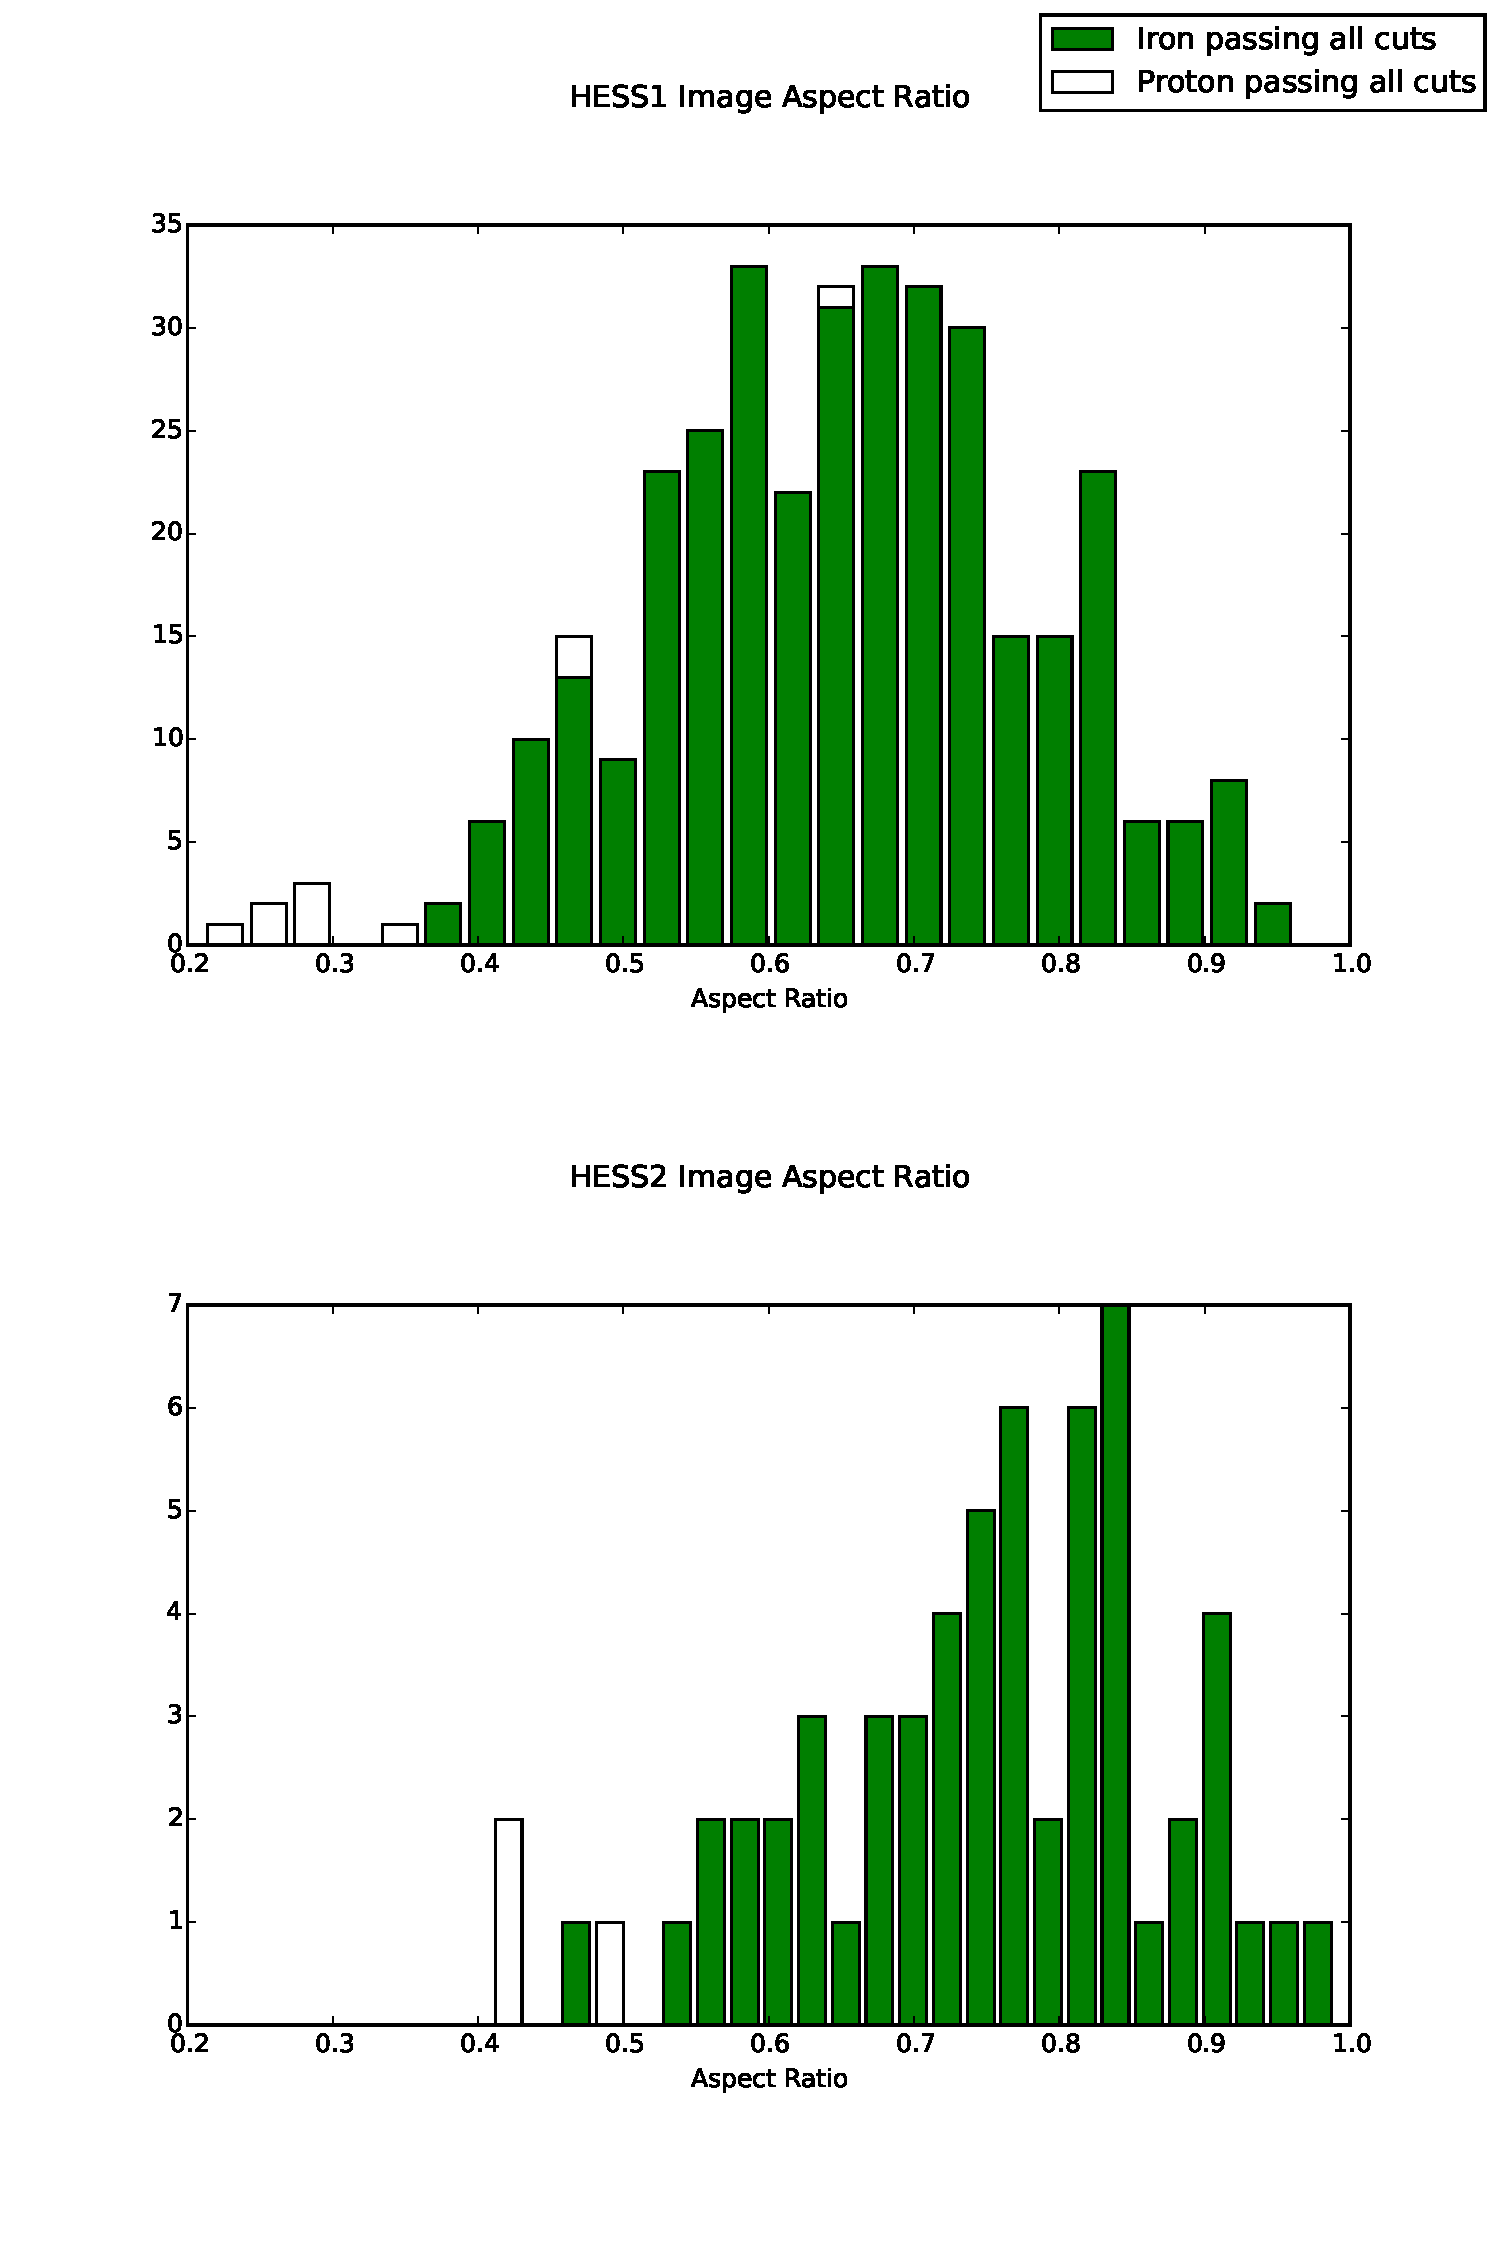
\includegraphics[width=0.9\textwidth]{aspectratio}
\caption{The aspect ratio of images in events which pass the multiplicity cut are shown. It is clear that the proton events have a strong tendency towards lower Aspect Ratios. We must remove the white proton pixels passing all other cuts, without removing dark green iron pixels passing all other cuts. A cut requiring Aspect Ratio $> 0.40$ should remove a large proportion of proton images without reducing the pass rate for iron nucleii.}
\label{fig:aspectratio}
\end{center}
\end{figure}

\begin{table}[h!]
  \centering
  \caption{Comparison of Proton and Iron Acceptance}
  \label{tab:protonacceptance}
  \begin{tabular}{ccc}
    \toprule
    & HESS1  & HESS2 \\
    \midrule
    Accepted Proton Pixels (\%) & 15.10 & 32.68\\
    Sample Purity (\%) & 10.1 & 5.1 \\
    \midrule
    High Multiplicity Accepted Proton Pixels (\%) & 0.83 & 1.03\\
    Sample Purity (\%) & 6.8 & 4.3 \\
    \midrule
    Accepted Proton Pixels after All Cuts(\%) & $< 0.06$ & $< 0.06$\\
    Sample Purity (\%) & / & / \\
    \midrule
    Accepted Iron Pixels after All Cuts(\%) & 2.44 & 1.66\\
    Sample Purity (\%) & 84.3 & 88.2 \\
    \bottomrule
  \end{tabular}
\end{table}

\subsection{Low-Energy Emission}
In the theoretical simulation of the LPD, we noted that the distribution in Figure \ref{fig:lpd} is only saturated in the region of around 35 TeV. Below this, the LPD is more heavily dependent on Energy, and thus our basic assumption of a characteristic equation will no longer be valid. However, we also know that any data sample will be dominated by lower-energy events as a result of the power law $\phi(E) \propto E^{-2.7}$. To account for this, an additional simulation of 15000 Iron events was conducted in the energy range 5-135TeV to give a realistic model for performance. The BDT remained the same, and the same initial cuts were replicated as before. The same was also done for Protons in the same energy range. 

We find that, for Iron Events, the acceptance rate falls by a factor of approximately 15. The relative proportion of HESS 1 to HESS 2 acceptance is broadly maintained at a factor of roughly 1.5, although the sample purity falls somewhat. If we account for the differing intergrated flux rate, we can calculate the ratio of expected high-multiplicity event rate $\Gamma_{HM}(E)$ for the ranges 5-135 TeV and 35-135 TeV.

\[ \frac{\Gamma_{HM}(5-135)}{\Gamma_{HM}(35-135)} = \frac{5^{-1.7} - 135^{-1.7}}{35^{-1.7} - 135^{-1.7}} 
= 30.3 \]

Thus, if we have thirtyfold increase in event rate, but only one-fifteenth of the original acceptance rate, we would ultimately expect that we would have twice as many Iron Events if the full energy range of 5-135 TeV was included. However, the low-energy proton acceptance is much higher than before at 0.21\%. Thus, were we to include all events in this energy range, we would again retrieve a sample dominated by protons. The results are summarised in Table \ref{tab:fullironacceptance}. 

\begin{table}[h!]
  \centering
  \caption{Comparison of Proton and Iron Acceptance}
  \label{tab:fullironacceptance}
  \begin{tabular}{ccc}
    \toprule
    & HESS1  & HESS2 \\
    \midrule
    Proton Pixels Accepted after All Cuts(\%) & 0.21 & 0.19\\
    Sample Purity (\%) & 1.74 & 0.00 \\
    \midrule
    Iron Pixels Accepted after All Cuts(\%) & 0.17 & 0.11\\
    Sample Purity (\%) & 80.00 & 80.00 \\
    \bottomrule
  \end{tabular}
\end{table}

Fortunately, there is a large degree of separability for Iron and Proton Events based on their Energy. The energy distribution of the Protons and Iron Events are shown in Figures \ref{fig:protonenergy} and \ref{fig:ironenergy}. The Iron distribution is slightly unusual, in that it is terminated above roughly 13 TeV, although lower energy events are much more frequent. This can be explained by the fact that the Cherenkov Emission Threshold is specified by the Energy per Nucleon, and Iron Nucleii have 56 nucleons. Thus, in almost all cases, Iron Nucleii below this Energy will interact with the atmosphere before they emit Cherenkov Light. The BDT is unlikely to identify 4 DC pixels with a sufficient $P_{signal}$ in an event without any real DC light, and thus no low-Energy High-Multiplicity Iron events are found. 

To remove the proton contamination from protons and non-saturated Iron events, we thus apply one additional Energy cut on the data sample. The majority of accepted protons have an Energy of less than 10 TeV, and the largest recorded Energy was 21.6 TeV. We can thus require that the reconstructed Energy is greater than 35TeV. This will, assuming a rough energy resolution of around 15\% in reconstruction, easily remove all of the proton background. We will also remove roughly half of the Iron events, but as shown in Figure \ref{fig:lpd}, this low-energy half of events will mostly contain non-saturated DC emission that would be harder to reconstruct.

\begin{figure}
	\centering
	\begin{subfigure}[b]{0.9\textwidth}
		\centering
		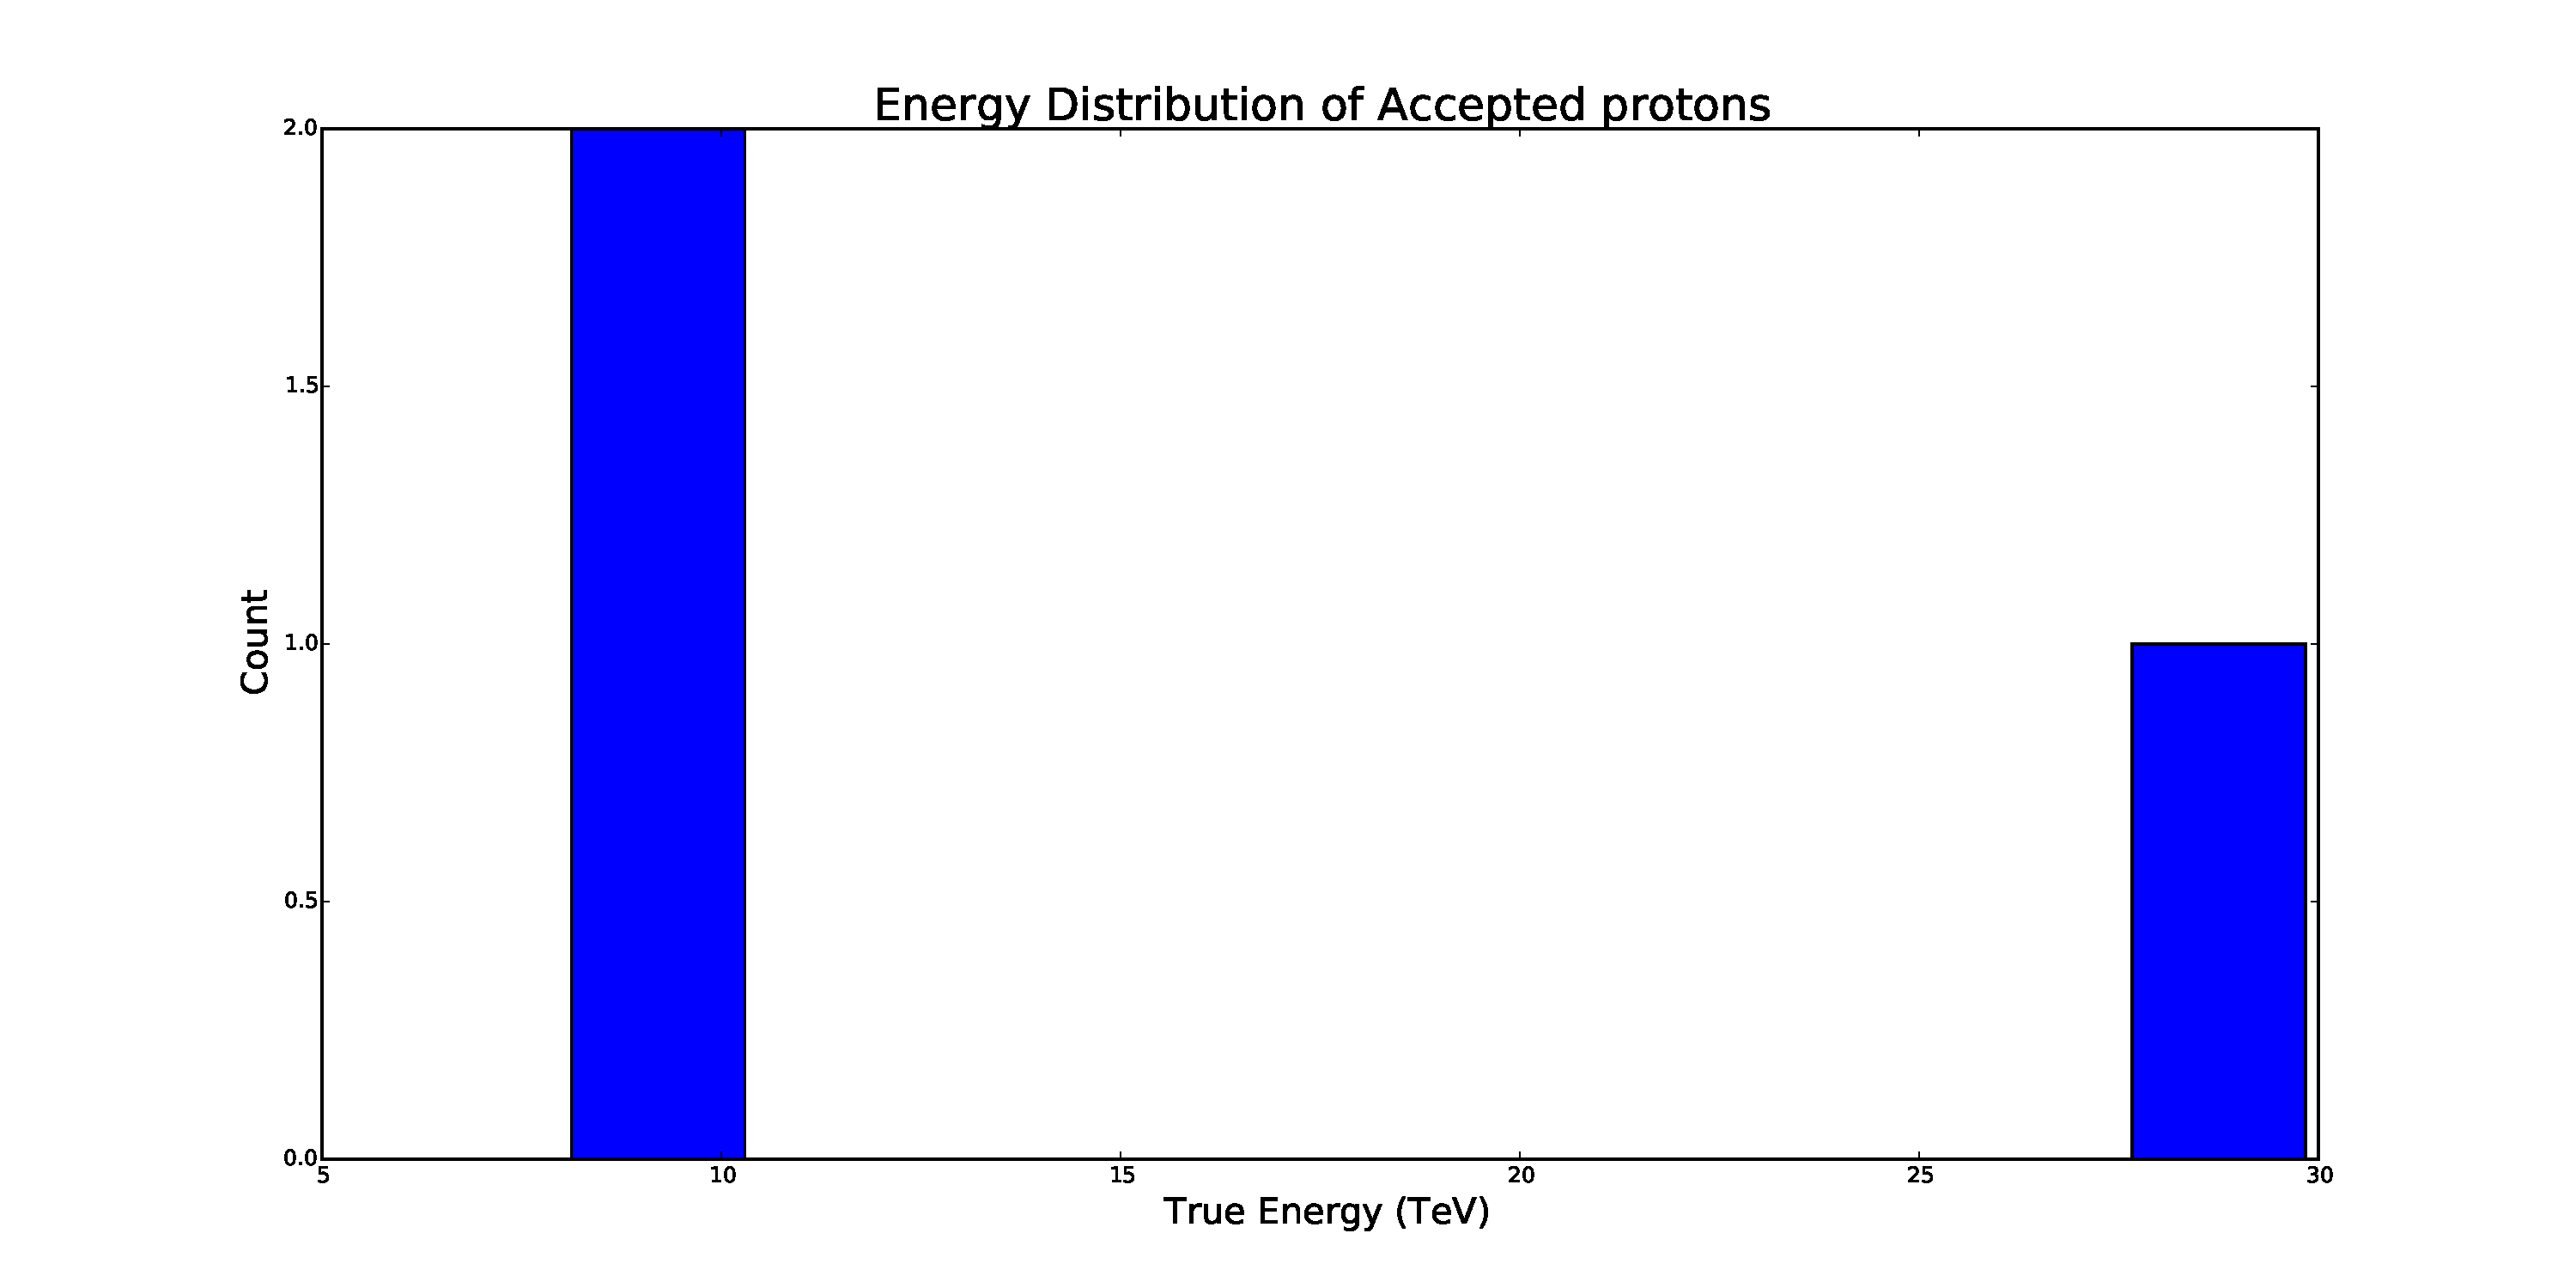
\includegraphics[width=\textwidth]{energyfullprotons}
		\caption{}
		\label{fig:protonenergy}
	\end{subfigure}
	\begin{subfigure}[b]{0.9\textwidth}
		\centering
		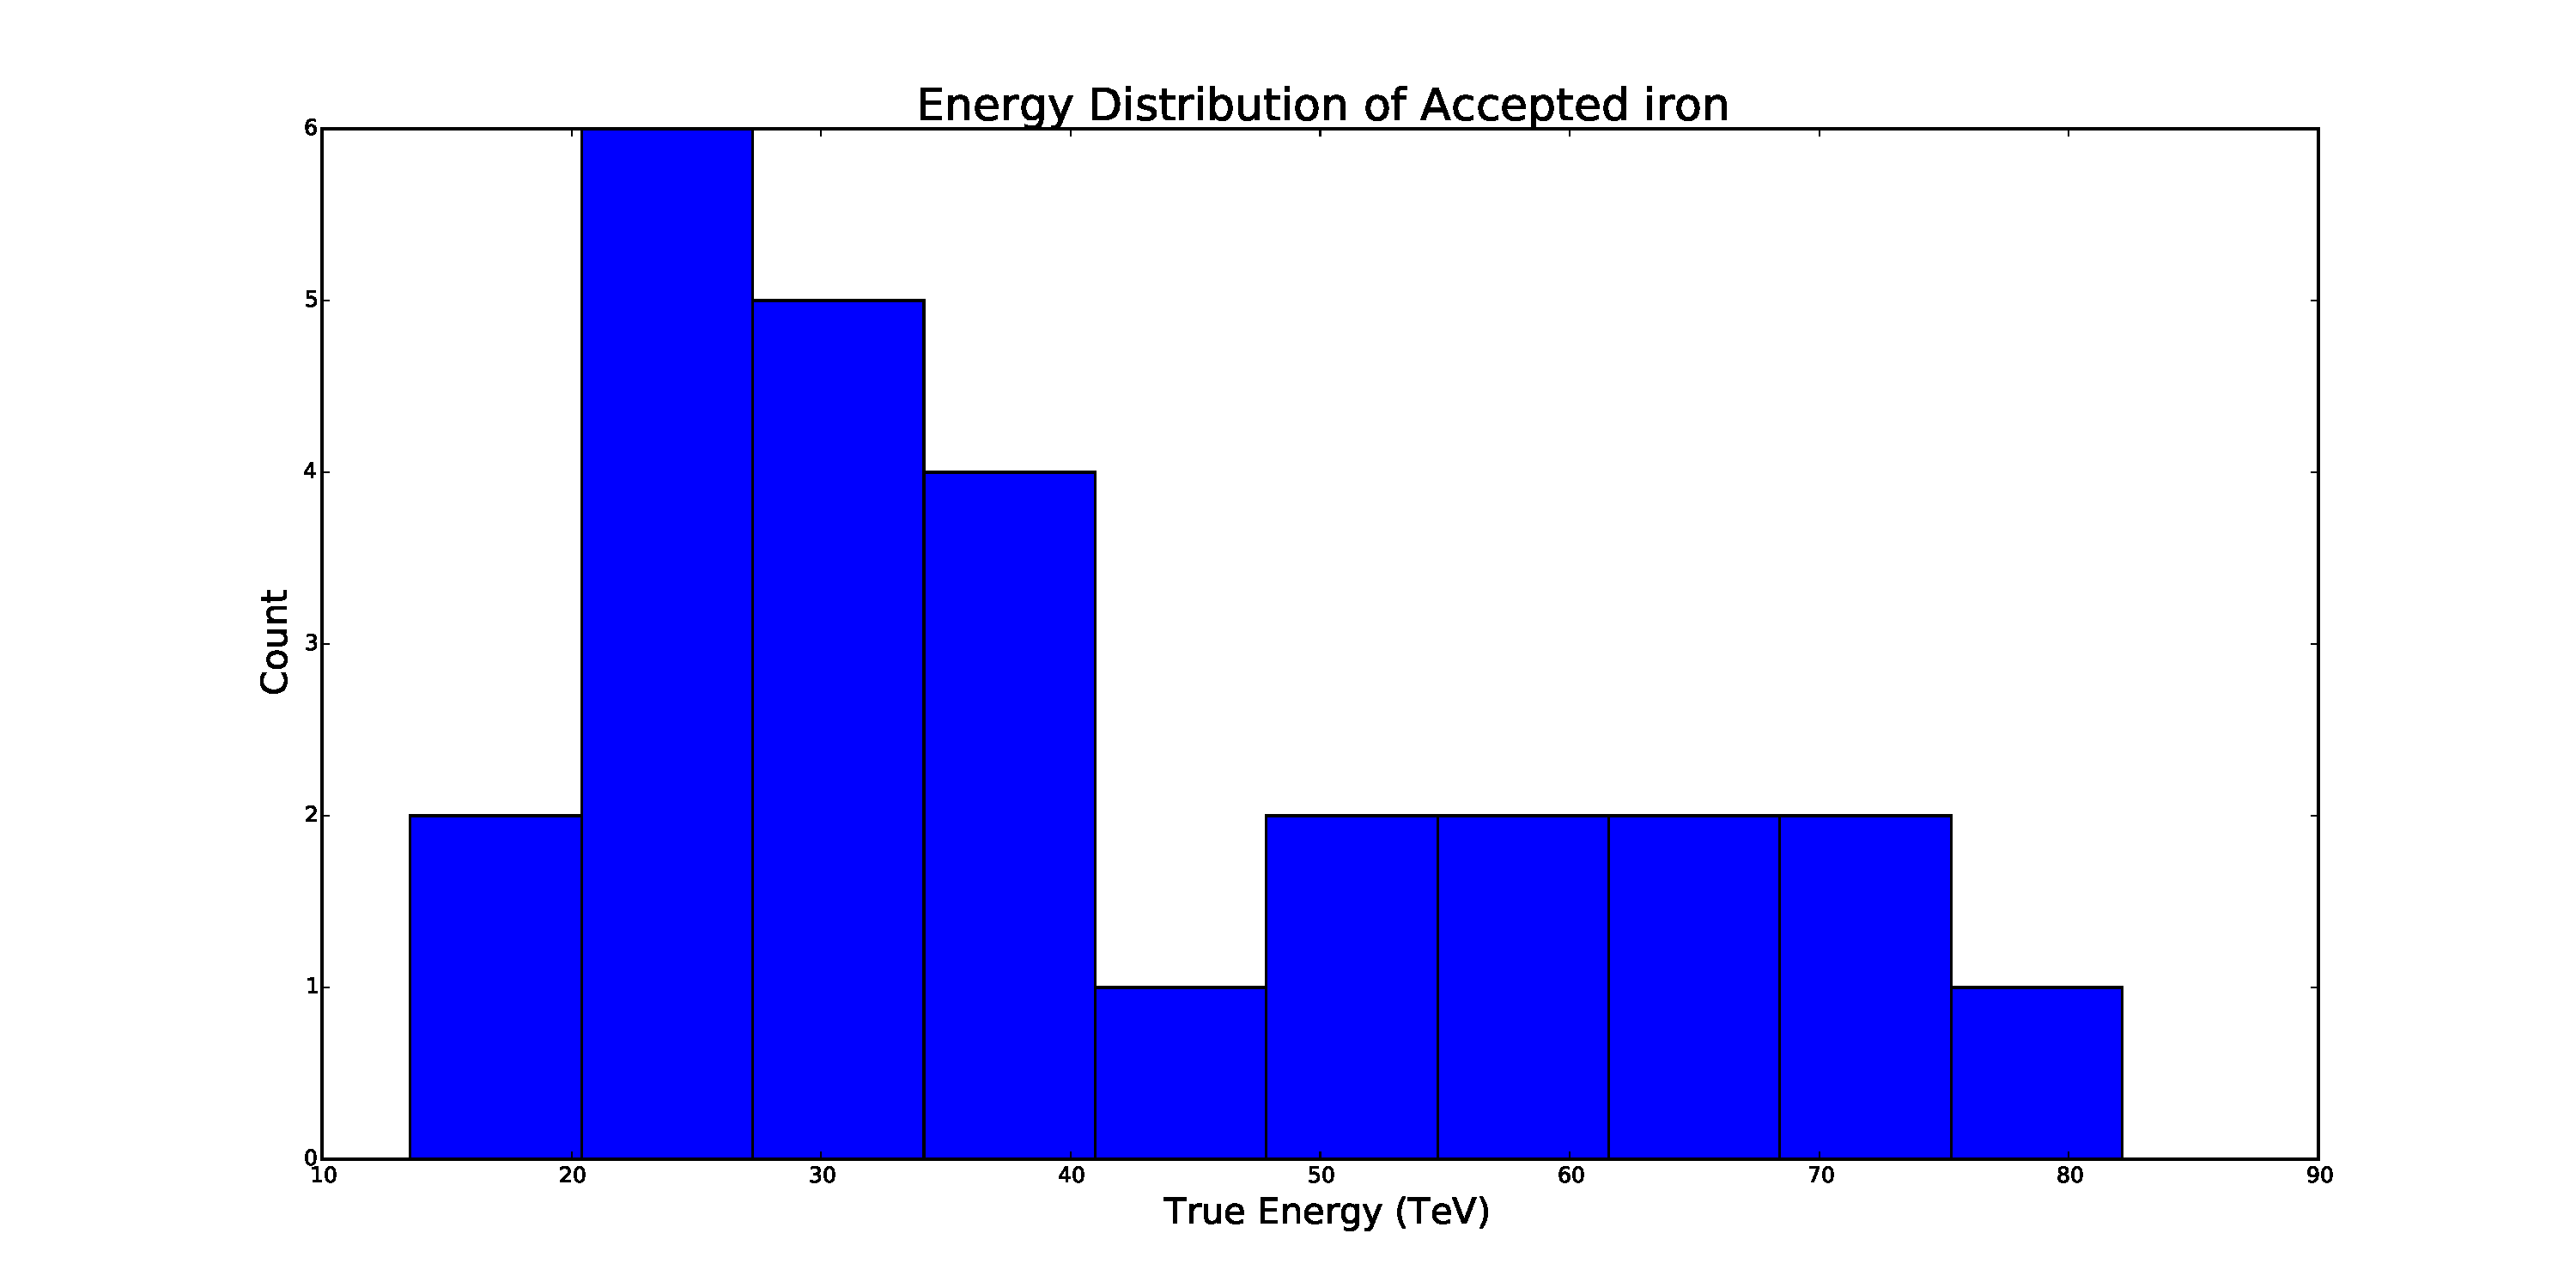
\includegraphics[width=\textwidth]{energyfulliron}
		\caption{}
		\label{fig:ironenergy}
	\end{subfigure}
	\caption{The Energy of Proton events passing all cuts is shown above in \ref{fig:protonenergy}. It is clear that the majority come from the low energy regime, and none have an energy greater than 22 TeV in. The Energy of Iron events passing all cuts is shown below in \ref{fig:ironenergy}. The majority come from the region above 20 TeV.}
\end{figure} 

\section{Parameterisation of the LPD}
Having identified DC pixels in a way that is both reliable and consistently removes background events, we can now consider the resultant LPD. We must parameterise this function before we are able to reconstruct events. We can also make use of the additional information provided by the EAS light in each shower image.

\subsection{Full-Shower LPD}
Having restricted ourselves to high-multiplicity events, we reduce our data sample to mostly images in which air shower lies relatively close to the center of the telescope field of view. We can conclude that in many of our images, the air shower should be mostly contained within the telescope image. In the same way as for DC light, we can firstly look for the existence of a Characteristic LPD describing the EAS Intensity, which we define as $I_{tot}$=Image Amplitude. The results for high-multiplicity events at various energies is shown in Figure \ref{fig:fullshowerlpd}.

\begin{figure}
\begin{center}
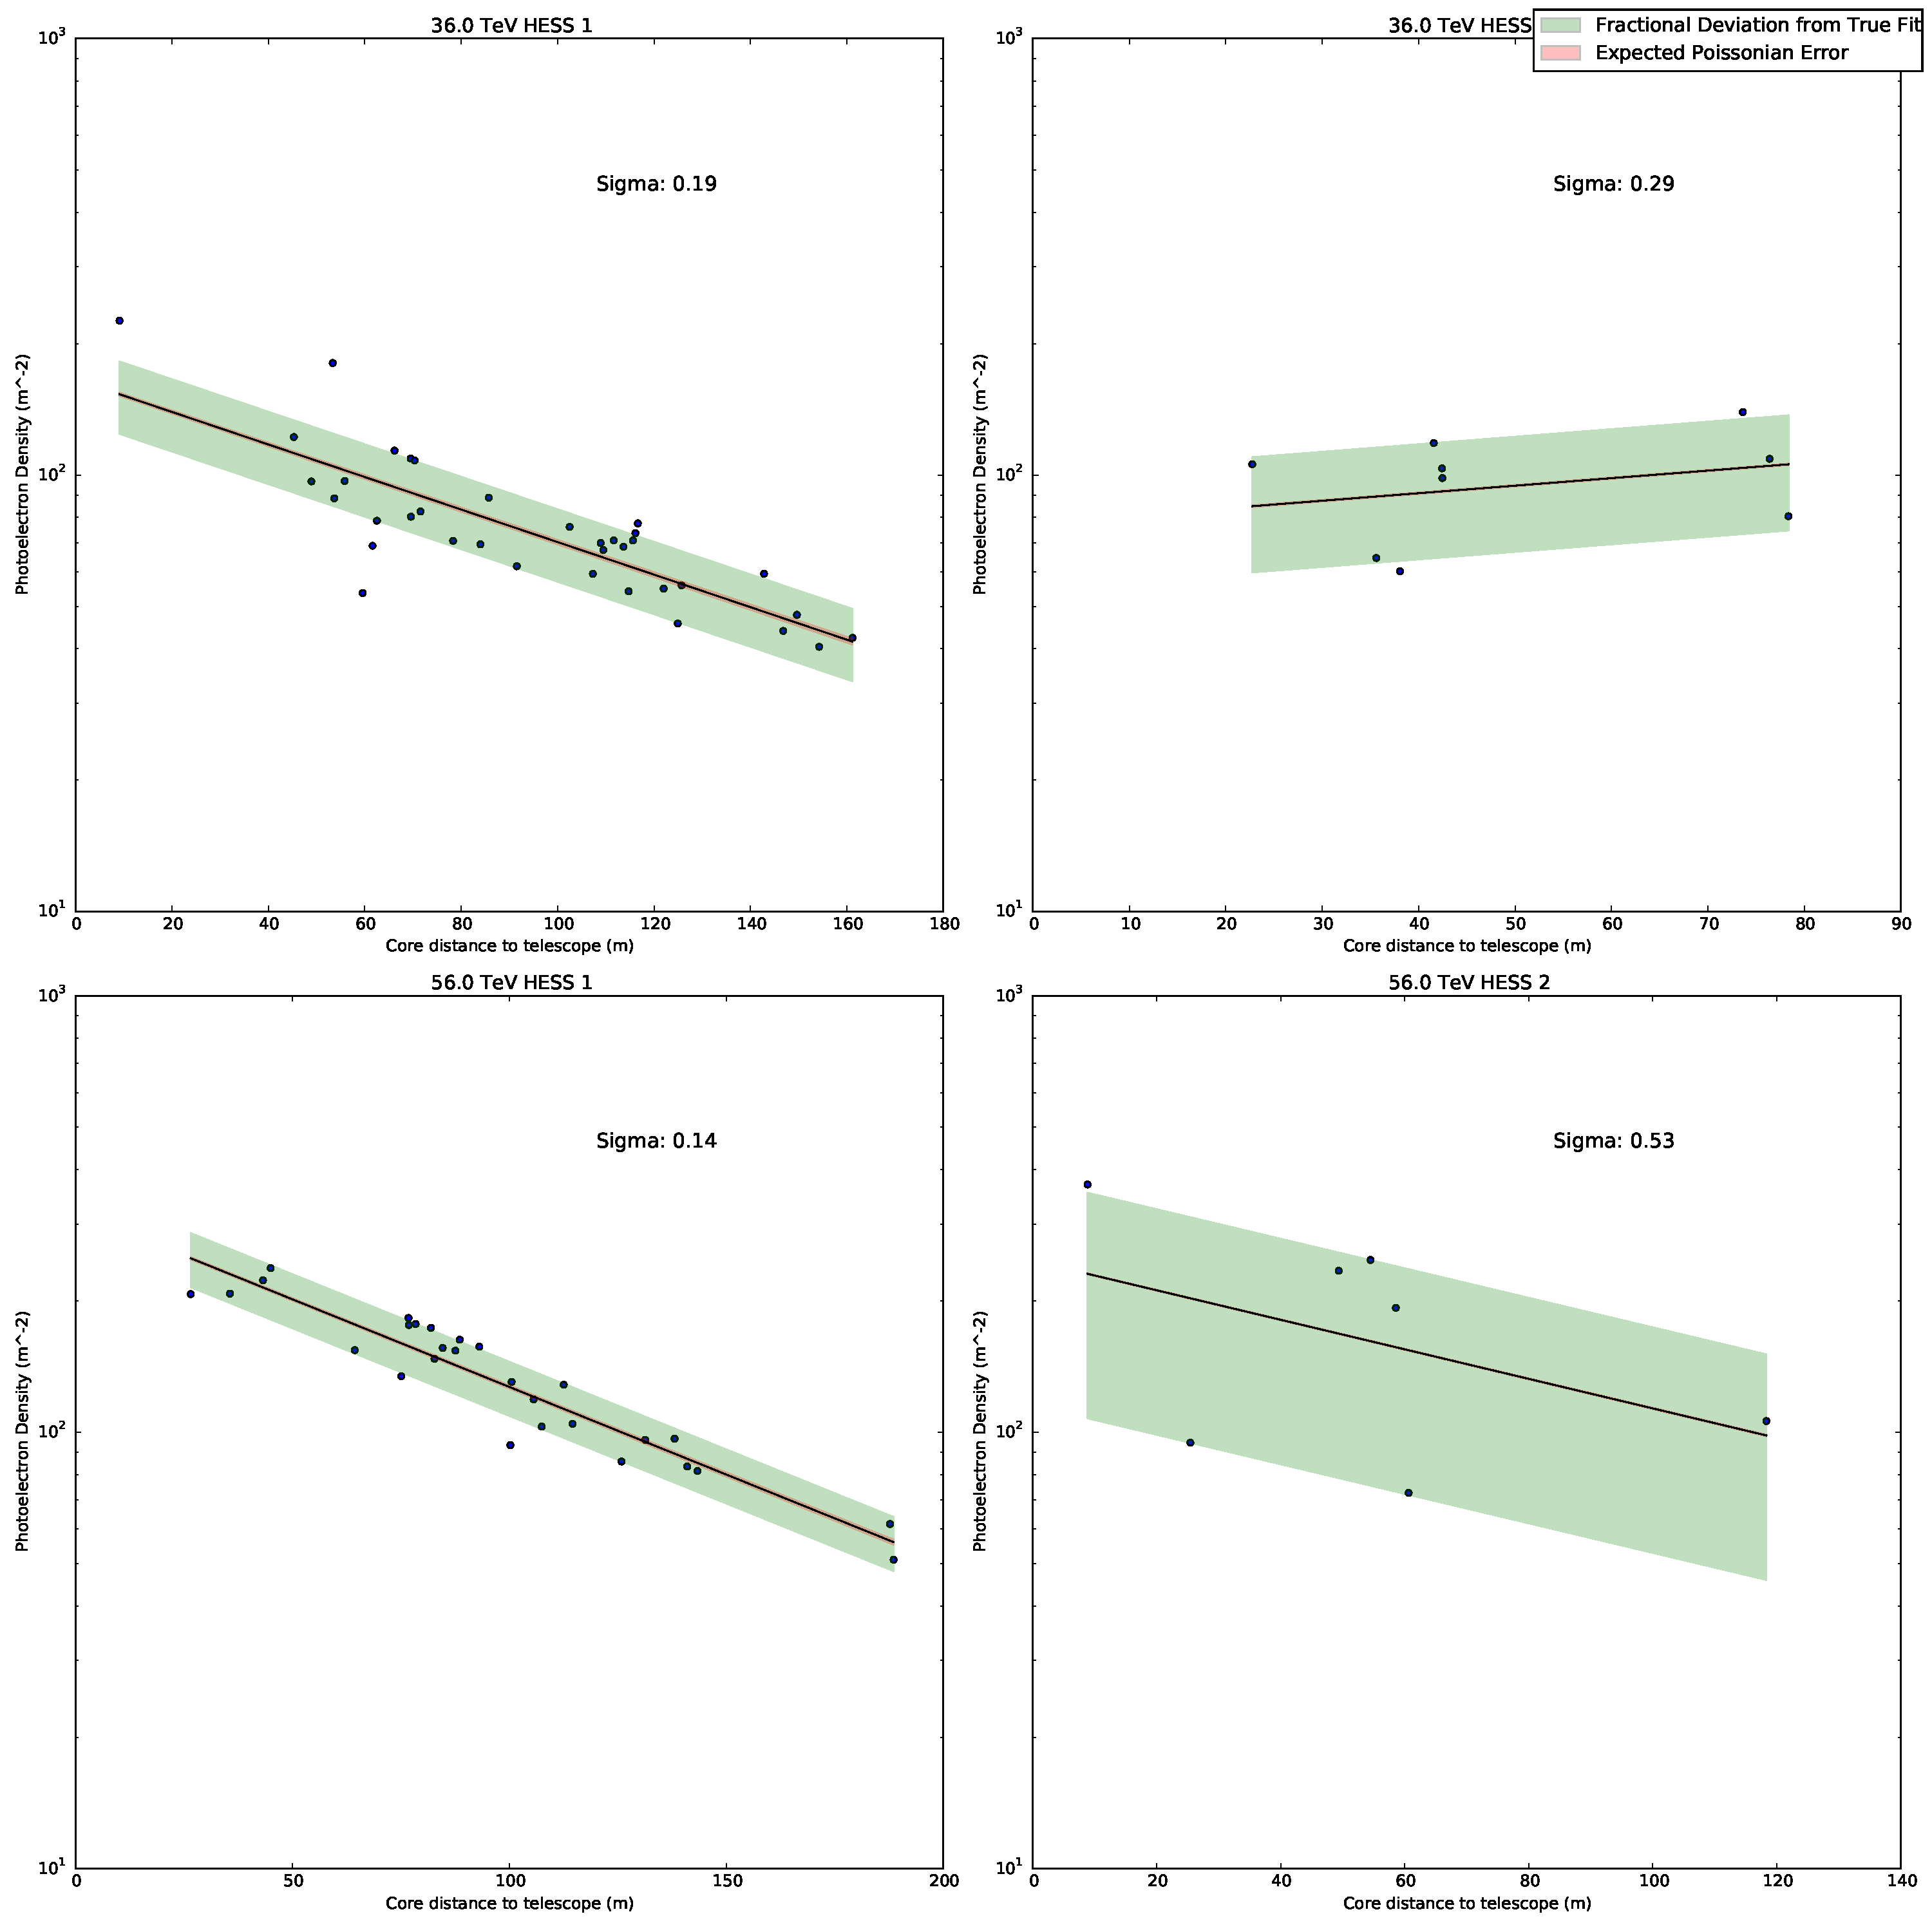
\includegraphics[width=\textwidth]{corsikafullshowerlpd}
\caption{The distribution of HESS 1 Image Amplitude is shown for various energies in the range 36-96 TeV. In each case, the exponential fit is indicated, along with the fractional deviation band in green.}
\label{fig:fullshowerlpd}
\end{center}
\end{figure}

For each energy, a clear exponential decay in Image Amplitude is observed. The data is fitted with a line of the form $y_{i} (x) =A_{i} \exp (K_{i} x)$. For the purposes of reconstruction, an exponential decay with a varying exponent and amplitude will not be particularly useful, because there are two degrees of freedom.

In order to overcome this, we can instead try to parameterise the exponential fits. Across all energies, a fit is made and the exponent coefficients are recorded. A plot of the $K_{i}$ exponent values is then made, as shown in Figure  \ref{fig:powerlawlpd}. The K coefficients follow a clear linear distribution, to which a line is fitted. We obtain an equation to determine the exponent of each power law. 

\[ K_{i} = K(E_{i}) = -0.00004 E_{i} + -0.00692 \]

Having retrieved a law for K, each dataset is then fitted a second time. The exponent is determined by the Energy, leaving only one degree of freedom for the fit. The fitted Amplitudes $A_{i}$ are then recorded, and are also plotted in Figure \ref{fig:powerlawlpd}. A clear relationship is again observed, this time an exponential law. A straight line is fitted to the logarithm of the data values, and we retrieve a second relationship describing the amplitude as a function of the Energy.

\[ A_{i} = A(E_{i}) =y =73.9 \times \exp (0.025 E_{i}) \]

Through combined use of the two equations, we can parameterise the entire Full-Shower LPD using only the Energy. These fitted LPDs are also plotted in Figure \ref{fig:fullshowerlpd}. The fractional deviation from the fit is found for each point by calculating $\Delta_{EAS} = \frac{fit_{EAS} - I_{tot}}{fit_{EAS}}$. We can then take the 68\% centile values to give us a $\sigma$-fraction width, and thus a fractional standard deviation $\frac{\sigma_{EAS}}{fit_{EAS}}$. The fractional standard deviation bands are shown in green, with a mean value of $\frac{\sigma_{EAS}}{fit_{EAS}}=0.15$ across the energies. We will make an approximation by assuming this value is a constant, though this is not strictly true. The Full Shower LPDs continue to be large enough to trigger telescopes for several hundred meters. It is thus likely that, for high-multiplicity events, we will obtain an additional four or five data points from the Full Shower LPD.

\[ y (x, E) = 73.9 \times \exp (0.025 E -(0.00004 E + 0.00692)x) \]

Although the Full Shower LPDs do not depend upon the charge of the primary particle, they will still enable the core position and energy to be effectively constrained. We can use the Full Shower LPD to obtain a rough estimate for the core position, and thus a rough estimate of the distance from each telescope to the core. Similarly the core energy can be estimated. Although this reconstruction will be inferior to one accounting for both LPDs, we can make use of the preliminary core position estimate to aid our calculation of $True_{DC}$. The information from the full-shower LPD will also be incorporated into our final likelihood minimisation, when we reconstruct the events.

\begin{figure}
\begin{center}
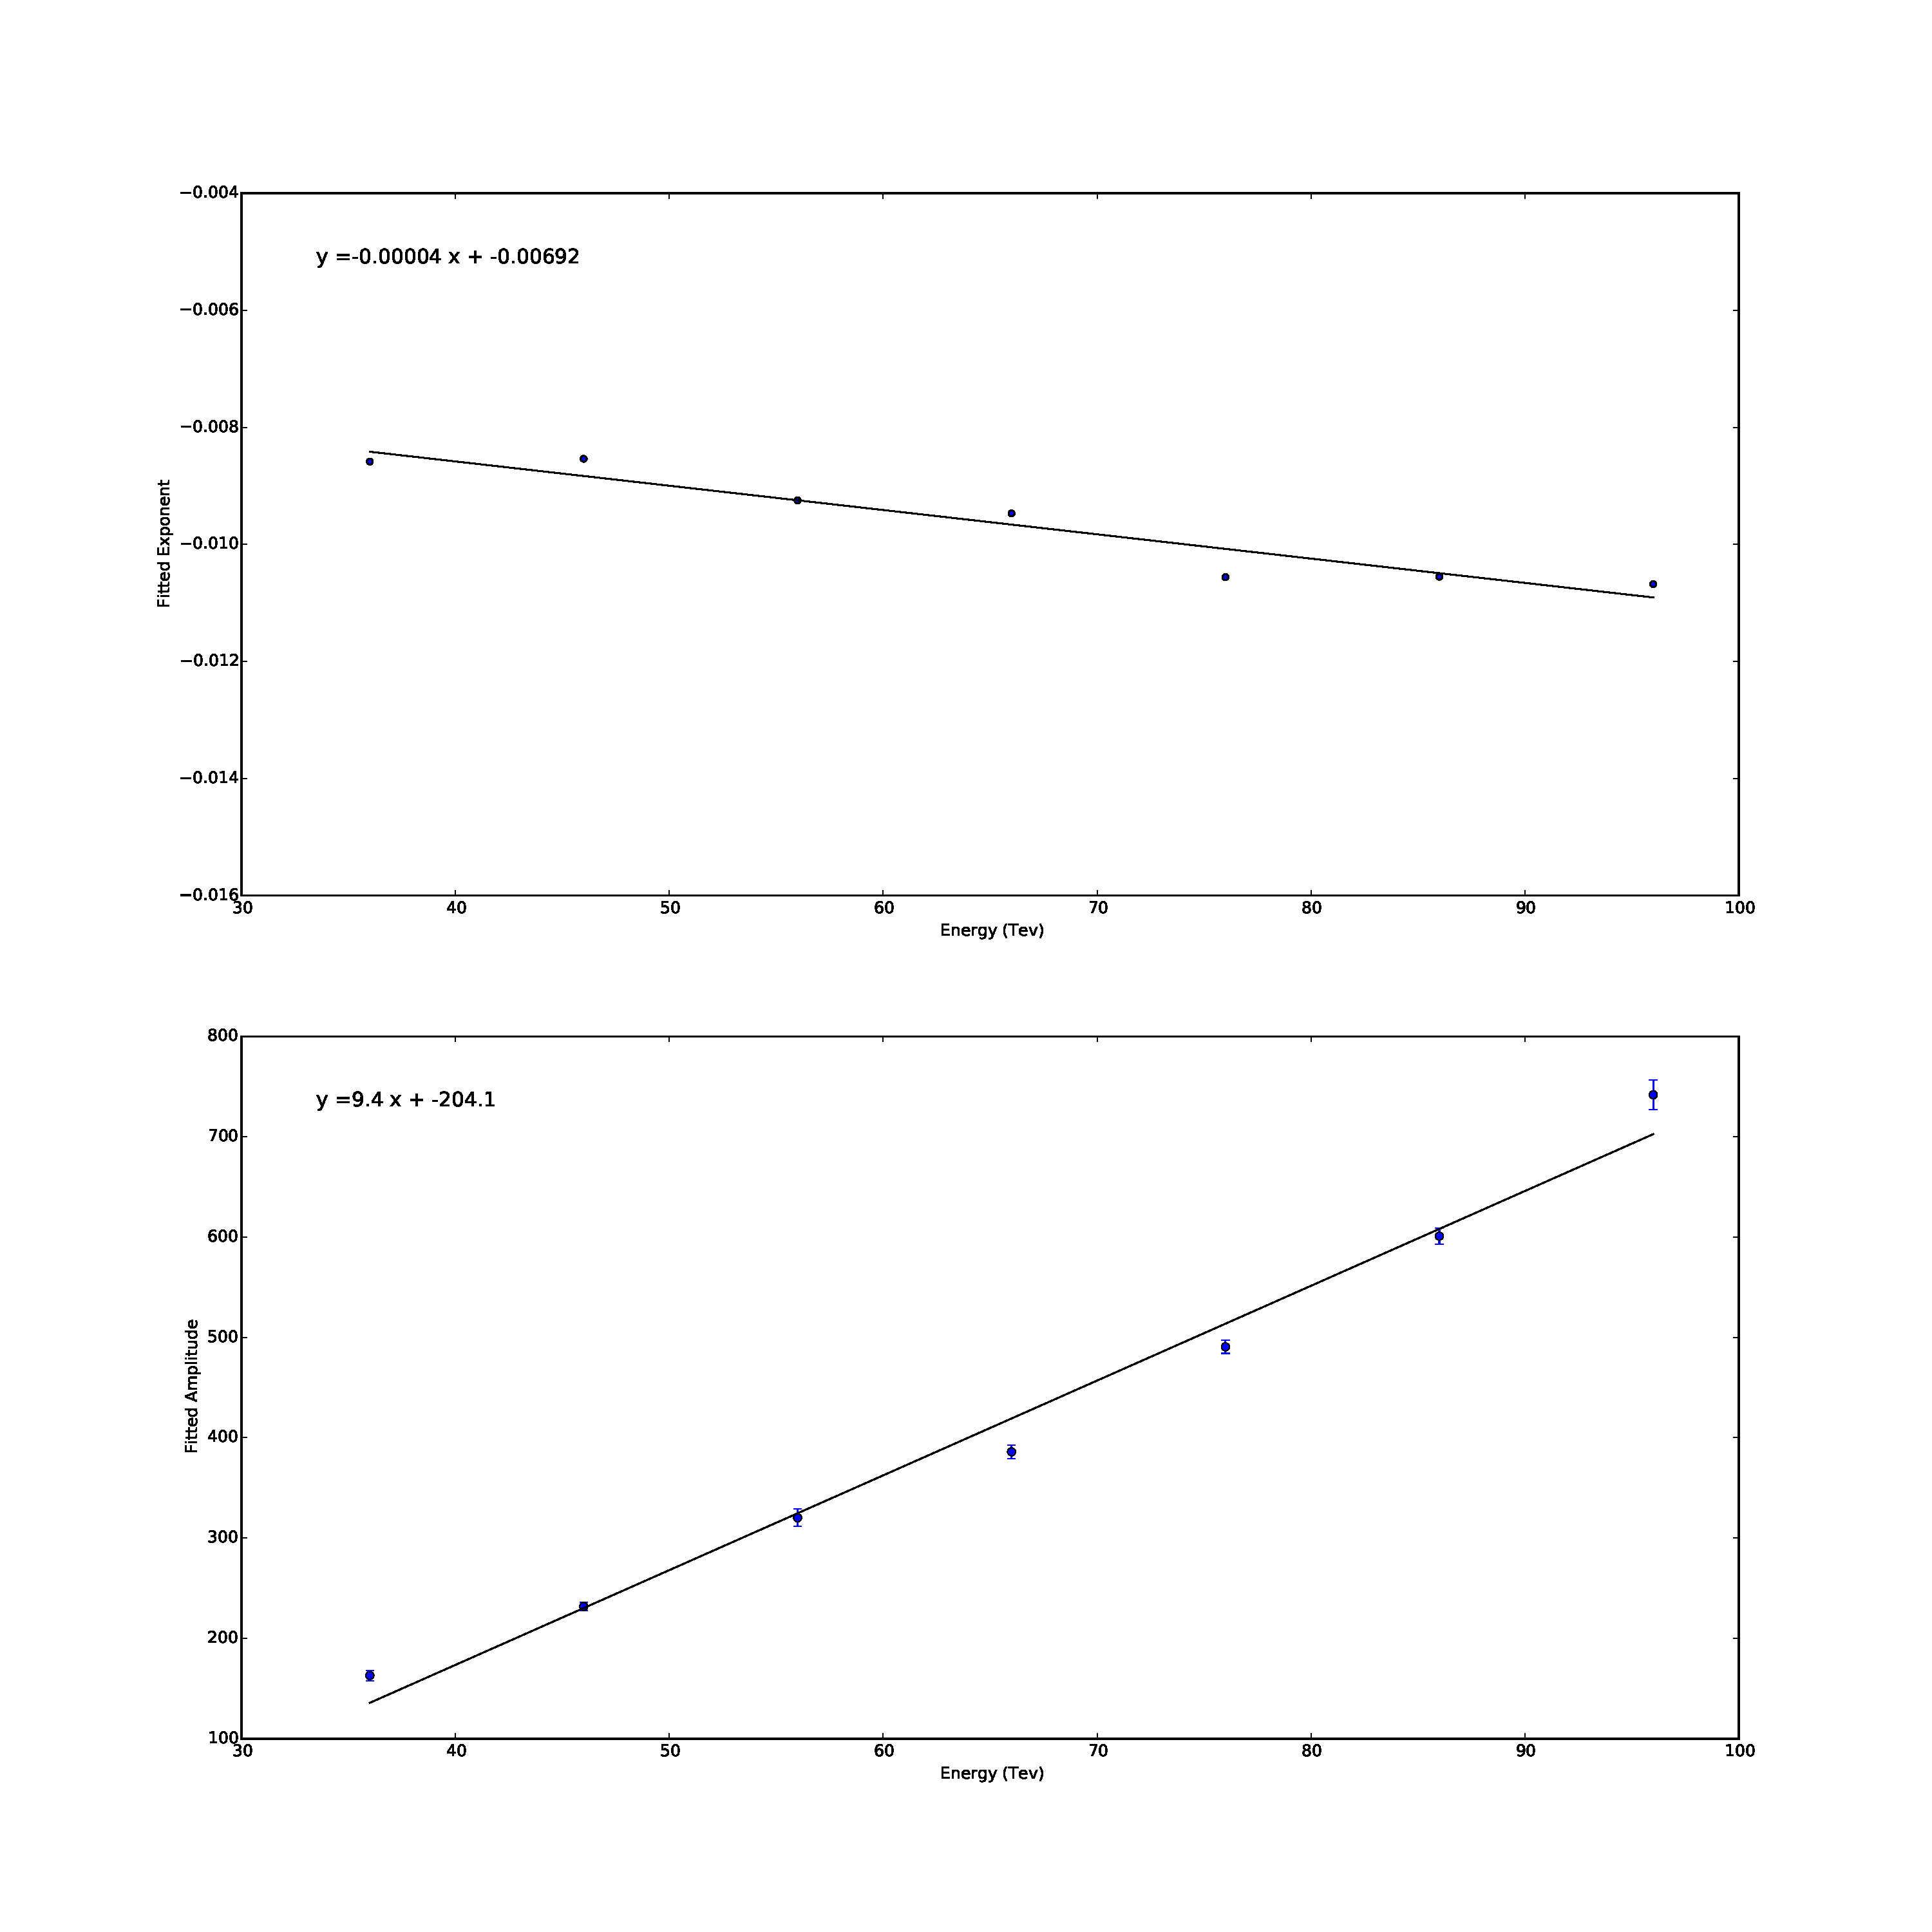
\includegraphics[width=\textwidth]{lpdpowerlaw}
\caption{The fitted exponents $K_{i}$ are shown above, along with the equation of the Fitted Exponent Line K(E). Once the fitted exponents are used, the resultant amplitudes $A_{i}$ are shown below, along with the fitted Amplitude Line A(E).}
\label{fig:powerlawlpd}
\end{center}
\end{figure}

\subsection{Determining $True_{DC}$}
Before we can extract the DC LPD from telescope images, we must first decide how to measure the quantity of DC light, $True_{DC}$. Determining the value of $True_{DC}$ is essential for determining the error in our LPD measurements. However, there are two natural ways of quantifying $True_{DC}$. In the basic case, we can simply consider the EAS-free intensity $Intensity_{max}$ in the DC pixel. An alternative is to take the entire EAS-free image amplitude $I_{tot}$ as our $True_{DC}$ value. The use of Image Amplitude accounts for the fact that the DC light is almost always split between two or more pixels. Although in most cases, one pixel has the majority of the light, in extreme cases the light can be evenly split between two. As a result of the smaller angular region covered by each CT5 pixel, this happens much more frequently for HESS2 than for HESS1. On the other hand, Image Amplitude measurement is susceptible to edge effects. A DC pixel lying near the image edge will be unaffected by this fact, but the total image amplitude may decline because dimmer pixels move over the image edge. We hope that, as with the full-shower LPD measurements, restricting ourselves to high-multiplicity events will enable us to remove most images that would otherwise suffer from edge effects.

To quantitatively compare the two methods, we can measure the error associated with both values of $True_{DC}$. A study of 2000 events was conducted, in which each cosmic ray was simulation without night sky background or EAS background. Each telescope image simulation was conducted twice, and difference between $I_{1}$ and $I_{2}$ was plotted as in Figure \ref{fig:simtelerror}. The fractional difference from the mean Intensity of an image was defined as $\Delta = 2 \times \frac{I_{2} - I_{1}}{{I_{2} + I_{1}}}$. 

For $I_{tot}$, it was found that the standard deviation in fractional difference was $\frac{\sigma_{Itot}}{I_{tot}}=0.06$, meaning that there is an inherent error of 6 \% in measurements of $True_{DC}$. This is reasonably low, and can be predominantly explained by the random nature of Photomultiplier Tubes (PMTs) that are used to measure the Photon Intensity in each pixel. In later calculations of the error in Intensity, this fractional error can be subtracted in quadrature. The distribution did not vary between HESS1 and HESS2 telescopes. For the alternative $Intensity_{max}$ measurement, the fractional standard deviation was $\frac{\sigma_{Imax}}{I_{max}}=0.09$ for HESS1 and $\frac{\sigma_{Imax}}{I_{max}}=0.12$ for HESS2, a clear increase. This implies that the $I_{tot}$ measurements are more reliable.

For an alternative measurement of error in the LPD, a simulation of 2000 events was conducted with a fixed energy of 56TeV. The interaction height was allowed to vary realistically. The true distance to core was recorded from Sim\textunderscore telarray, and a graph was plotted of DC pixel intensity against core distance. As expected, a characteristic LPD is observed, as seen in Figure \ref{fig:corsikalpd1}. Due to the trigger cut on HESS cameras of 20 photoelectrons, we are only able to see the LPD from around $r_{core} \textgreater 30m$, at which point the LPD intensity crosses the threshold of 20 p.e. All telescope images lying within the maximum DC radius $r_{max}$ are marked in black, where the value of $r_{max}$ varies with energy and first interaction height. We expect these events to follow the clear theoretical LPD observed in Figure \ref{fig:lpd}. After the first interaction, further emission be determined by a highly variable fragmentation process. These events are plotted in red, and will be ignored for LPD fitting purposes. 

A parameterisation of the form $y = A \exp (b x) + C $ is fitted to the measurements of $True_{DC}$. The fractional deviation $\Delta_{TrueDC} = \frac{signal_{fit} - True_{DC count}}{signal_{fit}}$ can then be found. Using the 68th centile of all absolute fractional deviations $\Delta_{TrueDC}$, we find that the HESS LPD for $I_{tot}$ has an error of $\frac{\sigma_{Itot}}{I_{tot}}=0.48$. Repeating for $Intensity_{max}$ calculated values, the resultant LPD had an error of $\frac{\sigma_{Imax}}{I_{max}} = 0.51$. Again, it is clear that $I_{tot}$ has a smaller associated error than $I_{max}$.

It is interesting to note that the values of $I_{max}$ and $DC_{count}$ are correlated with one another, more than with $I_{tot}$. The fractional standard deviation between $I_{max}$ and $DC_{count}$ is relatively small, at 0.34. It is found that the $I_{max}$ value, and by extension the $DC_{count}$ value, consistently underestimates the quantity of DC light in an image. This is not surprising, and indicates the degree to which DC light is often split between multiple pixels. As this effect is clearly not negligible, we choose to define $True_{DC}=I_{tot}$ for the rest of this analysis.

However, we know that in reality $True_{DC}$ will also have an associated error $\sigma_{STA}$. This error originates in the use of internal random numbers for Sim\textunderscore telarray simulations, and means that a given air shower is not completely reproducible. Having selected a method for determining $True_{DC}$, we can use the associated value of $\sigma_{STA}=0.06$. In later calculations of the error in Intensity, this fractional error can be subtracted in quadrature. 

\[ \sigma_{LPD}^{2} = \sigma_{calculated}^{2} - \sigma_{STA}^{2}  \]

\begin{figure}
\begin{center}
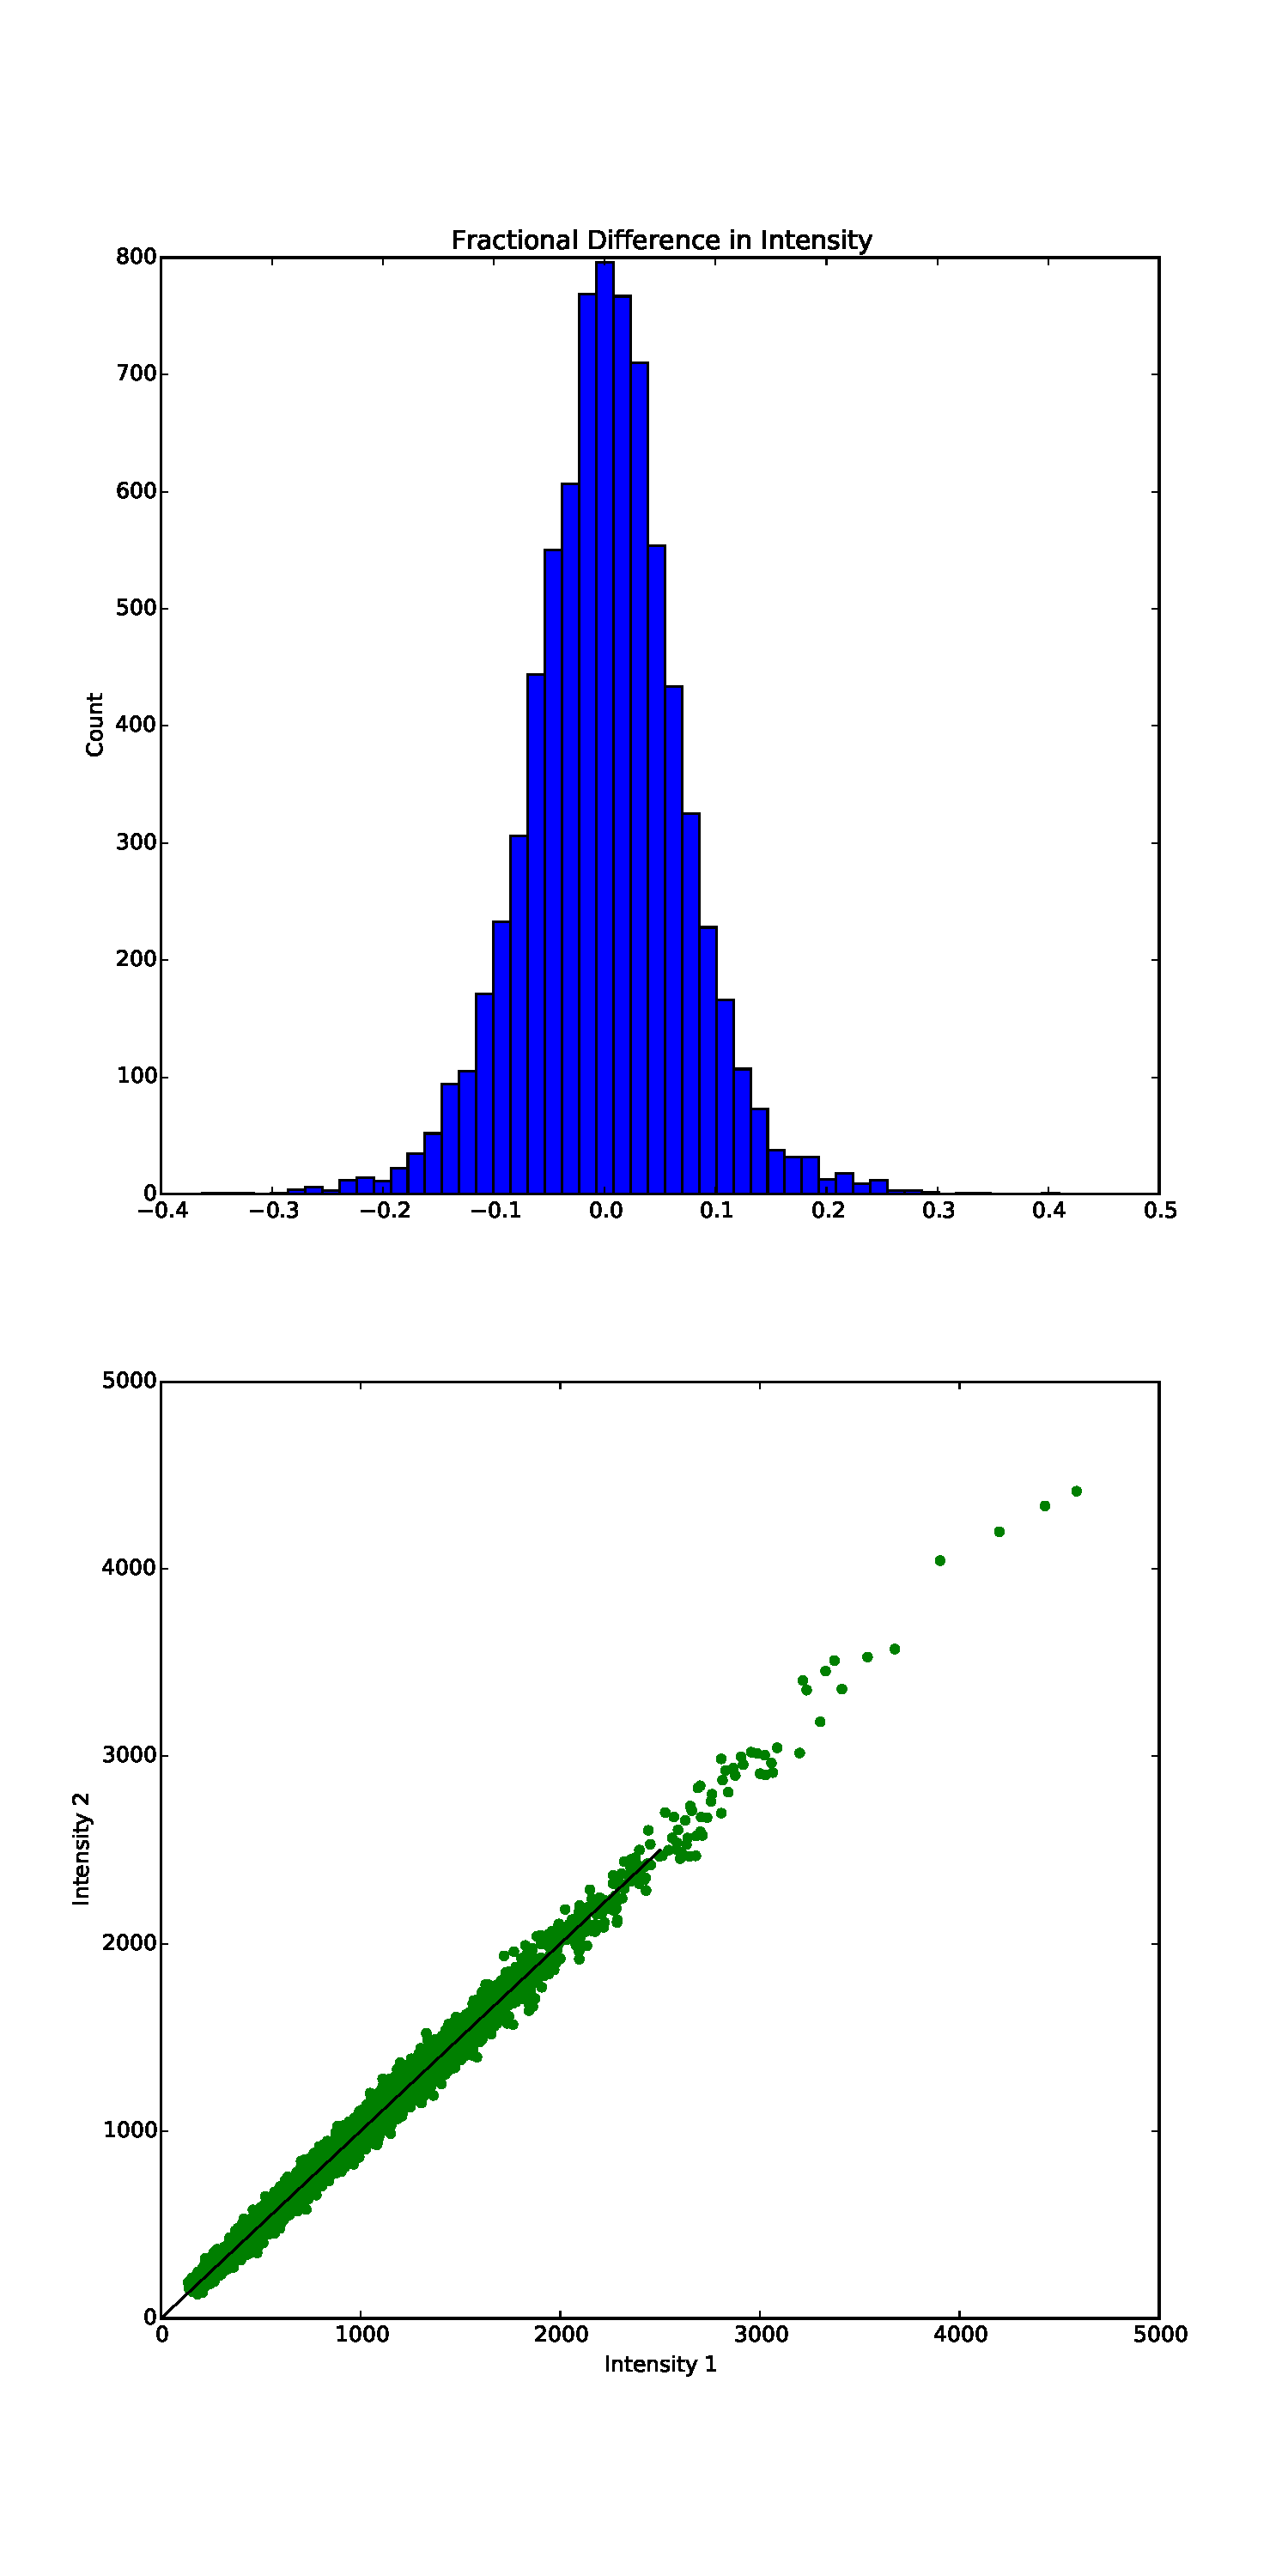
\includegraphics[height=0.9\textheight]{simtelerror1}
\caption{The fractional difference in total Image Intensity between the two simulations is shown in the graph above. A clear symmetric Gaussian is observed, with a mean of 0.00, and a standard deviation of 0.06. Below, the two intensities are plotted against one another. The distribution does not deviate significantly from the ideal 1:1 correspondence illustrated with the black line.}
\label{fig:simtelerror}
\end{center}
\end{figure} 

Taking account of $\frac{\sigma_{STA}}{I_{tot}}$, we deduce that the true associated error in the LPD is $\frac{\sigma_{TrueLPD}}{{True_{DC}}} = \sqrt{(\frac{\sigma_{TrueDC}}{True_{DC}}^{2} - \frac{\sigma_{STA}}{{True_{DC}}}^{2})} = 0.48$. Thus, we conclude that the error $\sigma_{STA}$ is broadly negligible, and in an ideal case, any LPD measuring pure DC light would always have a minimum error of 48\%. This is extremely large, and suggests that the atmospheric emission height may play a strong role in absorption of DC light. We had previously assumed that the amplitude of the LPD might not really be dependent of height. 

This suspicion was tested through a second simulation of 56 TeV Iron Events with a fixed interaction height of 20km. In this case, the recorded fractional standard deviation was $\frac{\sigma_{TrueDC}}{True_{DC}}=0.14$, a very significant improvement. This clearly confirms that there is a significant degree of LPD dependence of height, and that this far exceeds variations from small changes in charge number. Whether this will prevent us from using the LPD technique to reconstruct events depends on whether the measurements we make of the DC light will be independent of height. It may be possible to account for the varying interaction height.

One way of measuring the emitted DC light would be to use the variable $DC_{Count}$. The same fractional standard deviation calculations for varying first interaction height was repeated with this variable for the BDT candidate pixels in a full shower image, if the pixel had passed both the $DC_{Count}$ and $P_{signal}$ cuts. This provides a more reasonable estimate of the expected LPD error we are likely to be obtained experimentally, and also includes the additional complication of having incorrectly identified pixels in the dataset. As before, the fractional standard deviation of each pixel from the fit of the $True_{DC}$ LPD was found. Due to consistent underestimate of the $True_{DC}$ value using the simple $DC_{Count}$ method, the error was much larger, with $\frac{\sigma_{DCcount}}{DC_{count}}=0.43$ and the $\sigma_{STA}$ again being negligible in comparison. Interestingly, this is a slight improvement over the value of $True_{DC}$. It is likely that this is explained by the atmospheric absorption as a source of measurement uncertainty. Although the quantity of received DC light will be dependent on atmospheric absorbance, so will the EAS Shower Intensity that is present in the neighboring pixels. Thus, when subtracting the mean neighbouring Intensity of the DC pixel, the variation in $True_{DC}$ will be somewhat reduced. Despite the minor improvement, this representative error is extremely large, and will pose significant problems for event reconstruction. 

\begin{figure}
\begin{center}
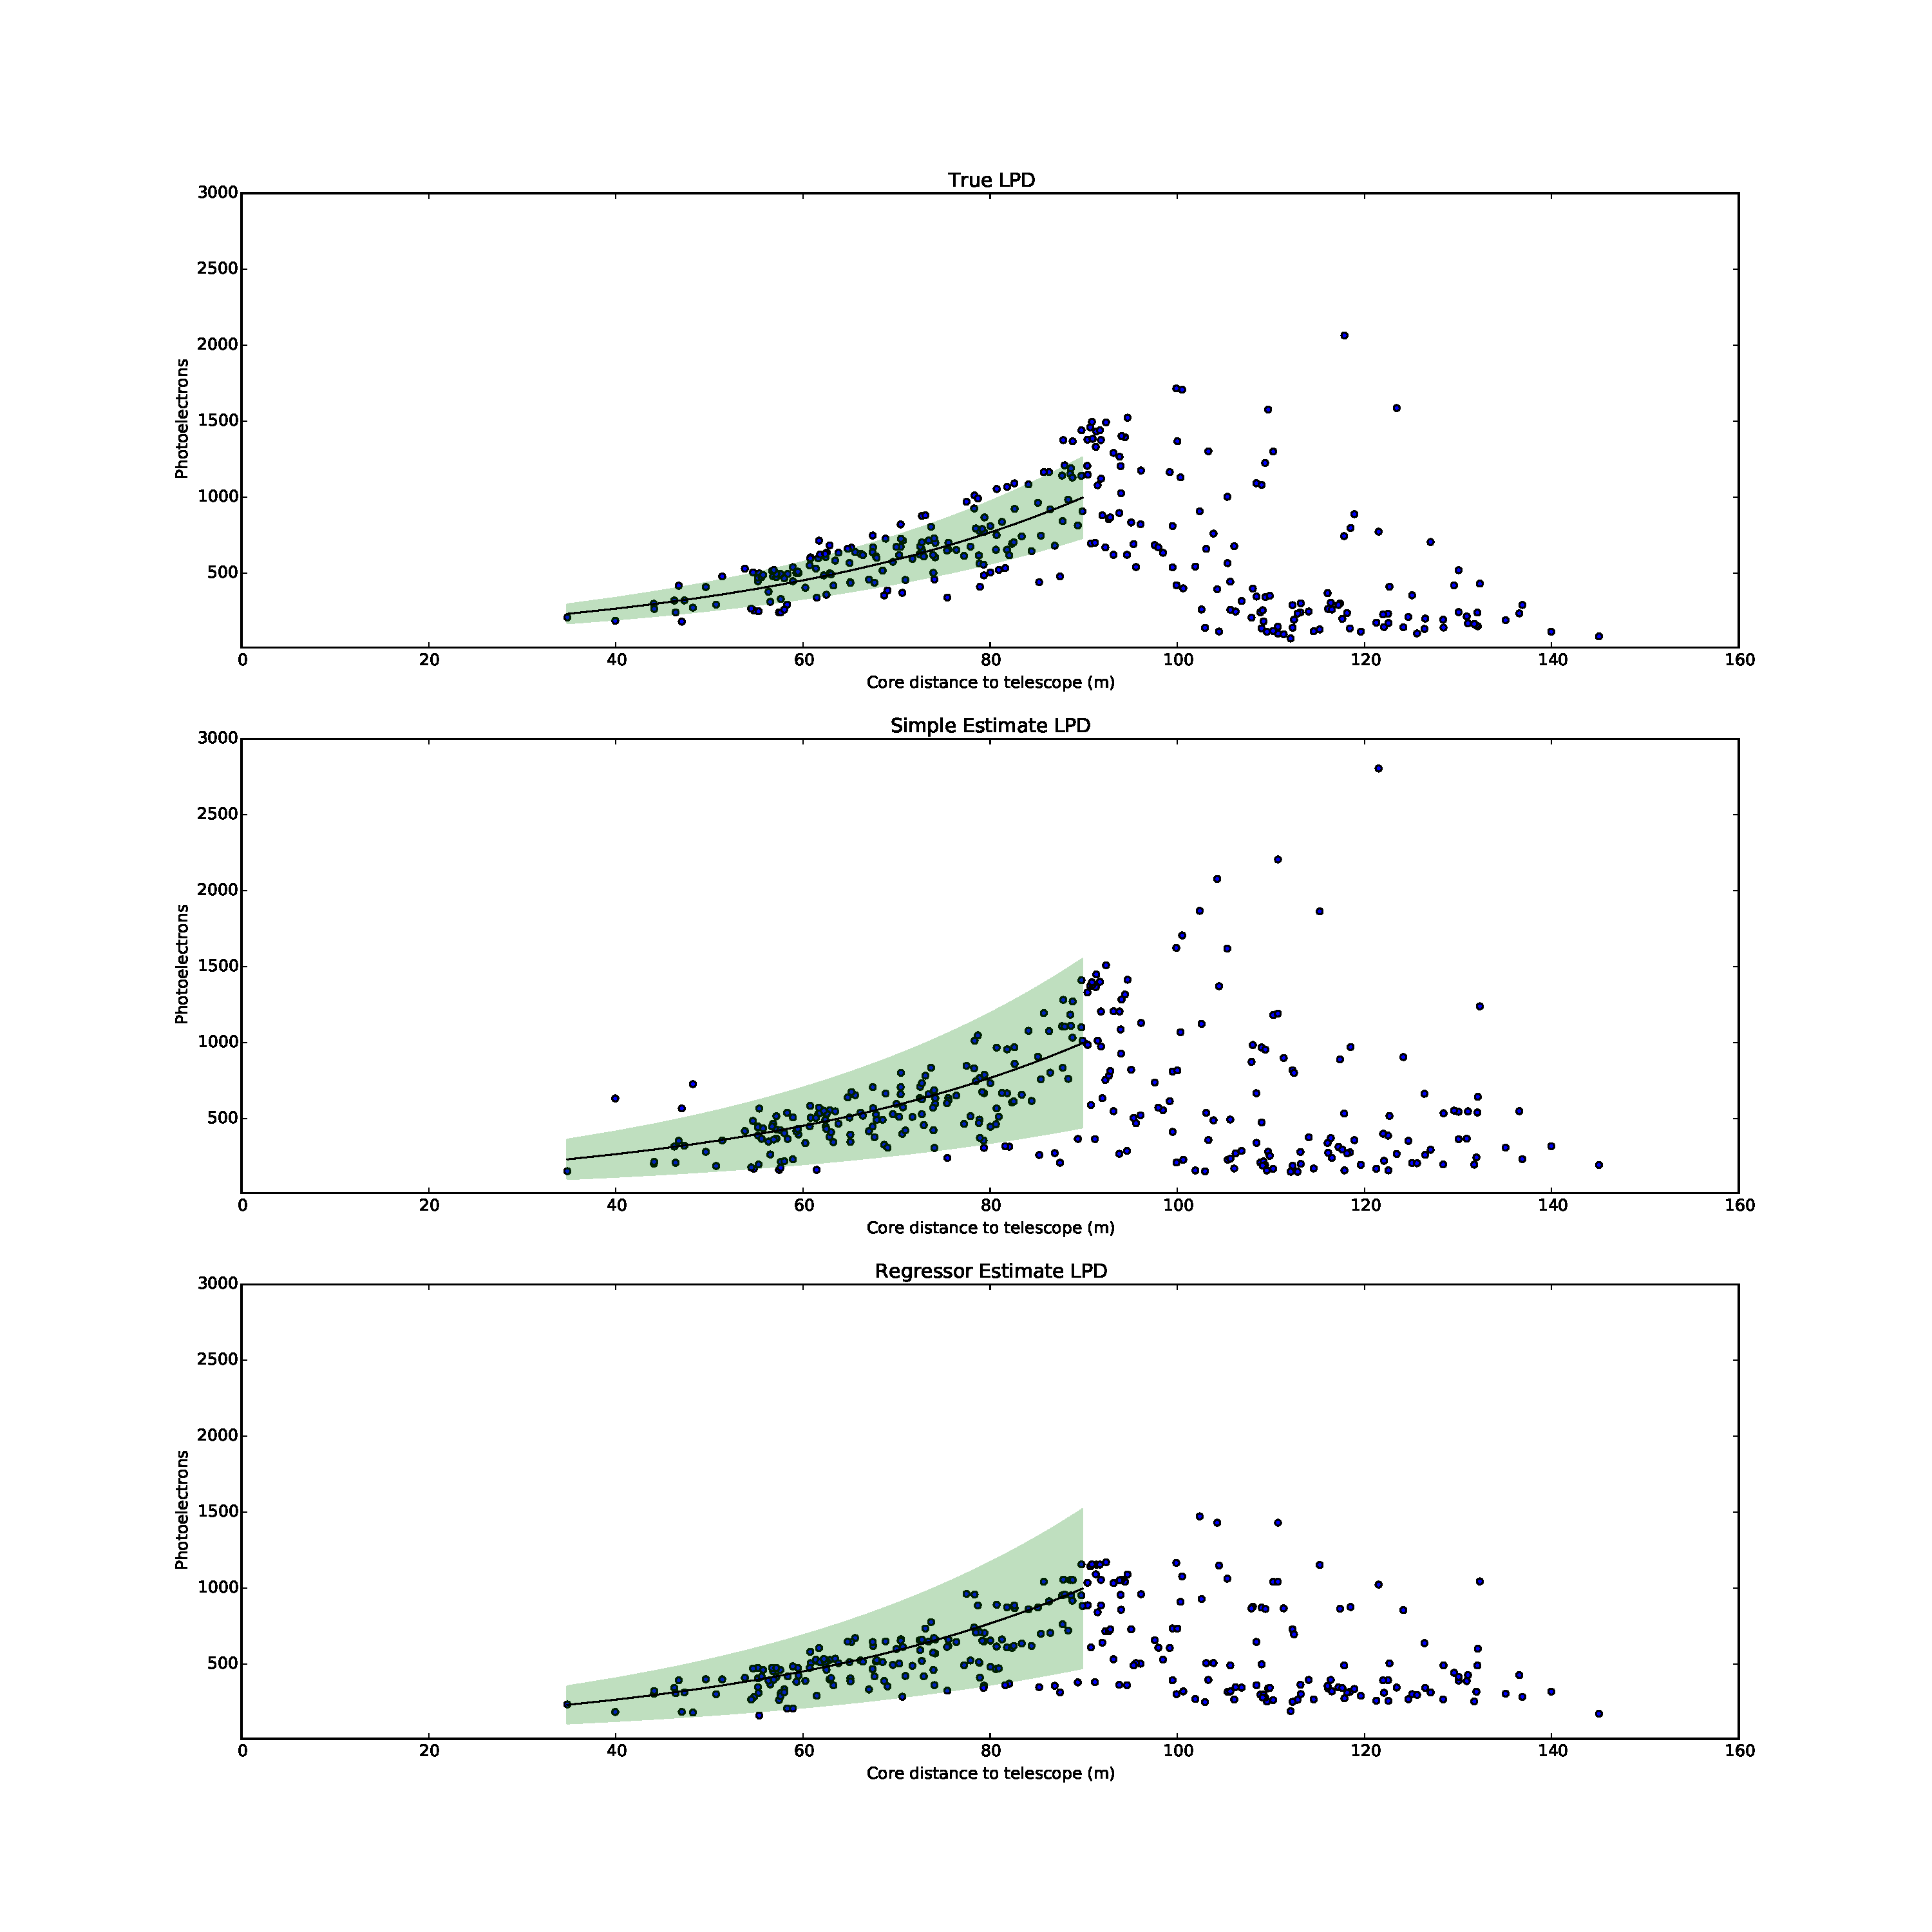
\includegraphics[width=\textwidth]{corsikalpd1}
\caption{The two LPDs shown above are estimates of HESS1 $True_{DC}$ calculated via $I_{tot}$, as well as for the maximum pixel $Intensity$. The two full-shower calculated LPDSs are shown underneath, with the simple guess $DC_{Count}$, and the regressor calculated $DC_{rgr}$. An exponential is fit to the $True_{DC}$ distribution, and the 68\% fractional deviation is shown in green. The same curve is shown on the two derived DC values, with the new fractional deviation being much greater.}
\label{fig:corsikalpd1}
\end{center}
\end{figure}

\subsection{Regression BDT for $DC_{Count}$}
In order to reduce the LPD error, an alternative method of calculating the DC signal was developed. Supervised machine learning was again used to solve the problem, through training of a BDT Regressor. As with Classifiers, Regressors are initially trained using individual data entries. Instead of the true classes for the entries, regressors require the true value of a continuous variable. Once trained, the Regressor can be used to predict a value of the variable for a given data entry. In this case, the Regressor is trained to estimate the quantity of DC light $True_{DC}$ for a given pixel. Once a DC pixel has been identified, the Regressor is applied to it. The Regressor returns the calculated value of $DC_{rgr}$, an alternative estimate of the DC signal. 

Training of a BDT is significantly impeded by the huge uncertainty in $True_{DC}$. A BDT regressor is unlikely to be able to improve upon the error in the original training values. To remove all associated uncertainty, a fitted parameterisation was used based on the LPD for $True_{DC}$ rather than the actual values of $True_{DC}$. The parameterisation, most importantly, will be independent of first interaction height. 

\[ y_{1}(r<r_{max}) = \frac{Z}{26}^{2} \times 5.3 \times \exp(0.013 r)\]
\[ y_{2}(r > r_{max}) = y_{1}(r_{max}) \times \exp (-0.06( r-r_{max})) \]

We train the regressor to interpolate the value of y(r) using a number of variables, and most importantly, we include the True distance to the Core and the true energy among the regressor variables. These values will be exactly known for the purposes of training, and known with a roughly 10\% uncertainty when an event is reconstructed. The full variable list in given in Table \ref{tab:regressor}. 

For convenience, an offset $C=-6.5$ in y(r) was omitted, yielding a simple exponential law. Counter-intuitively, it does in fact not matter whether the training values bear any direct relation to the $True_{DC}$ values. The only values that we need for reconstruction are our $DC_{rgr}$ values, based on the DC candidate pixel and full-shower image. As long as these $DC_{rgr}$ values are proportional to $Z^{2}$, the reconstruction method will remain valid. In theory, any parameterisation would be valid for the regressor to train with. It is obvious that, if given accurate core distance values, the regressor will always be able to perfectly replicate the exponential distribution. However, we cannot give a trained regressor true values of energy or distance to the core, when the regressor is applied to experimental images. Instead, we must give an approximation of these values, estimated through analysis of the full shower. Thus, if we were to choose a completely outlandish parameterisation that did not correlate to the images at all, the only useful variable would be the true core distance. As we do not exactly know the core distance, we would also have a large uncertainty in $DC_{rgr}$. Because no additional information would be present in the resultant LPD, any reconstruction would not provide reduction in core position or charge resolution measurement. 

If suitably trained, the regressor would consider the core position as a factor, but also correlate it with other variable related to the image. Then, given an estimate of the core distance, the regressor is able to produce a value of $DC_{rgr}$ with some small error, that is still proportional to $Z^{2}$. To be successful, we require the BDT to make of use of many other variables in addition to $DC_{count}$. If the BDT can do so, it will have a far smaller related uncertainty than the values of $True_{DC}$ by also taking the varying interaction height into account.

The training set of data for the BDT consisted of one true DC pixel entry in each full shower image. The training sample contains, in equal proportion, elements Manganese (Z=25), Iron (Z=26) and Cobalt (Z=27). This to ensure that the regressor is well trained to distinguish between different cosmic ray charges, by providing variation of $Z^{2}$ for training. If the regressor is capable of distinguishing between these three elements, then this will serve as a sufficient proof of concept. We expect that, were an entire spectrum of Cosmic Ray elements simulated, a regressor could be trained with similar performance for a large charge range. The training of such a BDT was not done as part of this analysis, due to computing time restraints. However, in Monte Carlo simulations, the existence of a regressor will be assumed.

As before, a separate BDT was trained to account for the differences in hardware for the CT5 camera. The Feature Importances for the HESS1 and HESS2 regressor are listed in Table \ref{tab:regressor}. There is little discrepancy in variable importance between the two BDTs.

\begin{table}[h!]
  \centering
  \caption{Relative Feature Importance in  Regressor BDT training}
  \label{tab:regressor}
  \begin{tabular}{ccc}
    \toprule
    Variable & HESS-1 & HESS-2 \\
    \midrule
    Aspect Ratio & 0.12 & 0.12\\
    $Intensity_{N.N.min}$ & 0.11 & 0.12\\
    Image Amplitude & 0.11 & 0.11\\
    $Q_{DC}$ & 0.10 & 0.11\\
    $r_{core}$ & 0.10 & 0.10\\
    $Intensity_{N.N.max}$ & 0.10 & 0.10\\
    $Mean_{N.N}$ & 0.10 & 0.09\\
    Energy & 0.09 & 0.09\\
    $DC_{Count}$ & 0.09 & 0.09\\
    $Intensity$ & 0.08 & 0.08\\
    \bottomrule
  \end{tabular}
\end{table}

The features importances are, on the face of it, rather surprising. Ultimately, the true values for energy and $r_{core}$ are not the most important variables. We can conclude that the regressor has been well taught to indirectly infer the cosmic ray charge, and account for this by correlating values to the true core distance/energy. The Aspect Ratio is heavily dependent on distance to core, but also on the charge. Thus, in combination with $r_{core}$, the charge can be reasonably inferred. Similarly the Image Amplitude is relied upon to infer energy, and in conjunction with the estimated energy, can indicate charge. It is encouraging to see that the regressor relies more heavily on Image Amplitude and Aspect Ratio, because these two values are known with a much smaller uncertainty than the core position/energy.

Repeating the comparison for the HESS1 regressor, we find for $\frac{\sigma_{rgr}}{DC_{rgr}} = 0.14$, a significant improvement over $\sigma_{DCcount}$. The plotted LPD is seen in Figure \ref{fig:corsikalpd1}. Through use of a well-defined law for the training values, we have eliminated the influence of $\sigma_{STA}$ on the training process. The comparative performance is recorded in Table \ref{tab:lpderror}.

Instead of rejecting DC pixels which do not meet out $DC_{count}$ and $P_{signal}$ cuts, we can separately measure their deviation from the LPD. In this way, we can include the information from these DC pixels in later analysis, while accounting for the larger uncertainty in their LPD measurements. For images which do pass only the multiplicity cuts, but not the $P_{signal}$ or $DC_{count}$ cuts, we find that the regressor error is $\frac{\sigma_{rejected}}{DC_{rgr}}=0.15$. It would be interesting to incorporate the information from these pixels into reconstruction, but doing so would remove our ability to constrain the core. Further study could attempt to use the rejected pixels, though the performance of the regressor on images without DC light would first need to be thoroughly tested to account for the possibility that rejected pixels belong to images without DC light. Because the BDT regressor functions as a Black Box, it is difficult to know how it is using the information from camera images to calculate $DC_{rgr}$. To ensure the validity of our Monte Carlo simulation, we will omit the rejected pixels as part of this analysis. 

\begin{table}[h!]
  \centering
  \caption{Fractional error from fitted 56-TeV LPD distribution}
  \label{tab:lpderror}
  \begin{tabular}{ccc}
    \toprule
    & HESS1 & HESS2\\
    \midrule
    $\sigma_{TrueDC}$ & 0.48 & 0.61\\
    $\sigma_{DCcount}$ & 0.43 & 0.58\\
    $\sigma_{rgr}$ & 0.14 & 0.16\\ 
    $\sigma_{rejected}$ & 0.15 & 0.17\\ 
    \bottomrule
  \end{tabular}
\end{table}

\section{Monte Carlo Simulation}
Having obtained a parameterisation for both the full and DC LPD, as well as the associated error in the case of a HESS-type array, the charge reconstruction technique can be applied to a simplified Monte Carlo simulation of the HESS array, developed as part of this analysis. Conducting a Monte Carlo simulation using the Gaussian-smeared LPD, we can measure the effectiveness of the LPD-reconstruction technique. The simulated Cosmic Rays must be high-multiplicity, and have a realistic distribution of energy and interaction height values.

\subsection{Iron Flux and Energy}
Iron nucleii, like all Cosmic Rays, follow a well-defined power law where $\phi(E) = \frac{dN(E)}{dt} = \phi_{0} (\frac{E}{TeV})^{-\gamma} $ for some constant $\gamma$ \cite{hess07}. Using the SIBYLL model for Cosmic Ray Simulation, we assume that $ \gamma = 2.76 \pm 0.11 $ and $\phi_{0}=0.029 \pm 0.01 m^{-2} s^{-1} sr^{-1} TeV ^{-1}$ \cite{hess07}. Considering the same Energy Range of 35-135 TeV, we can calculate the integrated Iron Flux. 

\[ F(35-135TeV) = \int_{35}^{135} \phi_{0} (\frac{E}{TeV})^{-\gamma} dE = \frac{\phi_{0}}{1.76}[35^{-1.76} - 135^{-1.76}] = 2.86 \times 10^{-5} m^{-2} s^{-1} sr^{-1}\]

Within CORSIKA, a square simulation of 300 x 300m was simulated. We can consider an identical $90000 m^{2}$ target region for core position simulation. The HESS telescope additionally has a solid and field of view of 5 degrees (0.006 steradians),meaning an expected telescope array Iron Flux of $F(35-135TeV) = 0.0154 s^{-1}$. On the basis of efficiency calculations in DC pixel identification, it is clear that 2.3\% of Iron Ray events will produce high-multiplicity DC pixels accepted by the BDT. Thus, we will ultimately obtain an hourly flux of $F(35-135TeV) = 3.40 \times 10^{-4} s^{-1} = 1.22 h^{-1}$ high-multiplicity Iron events. 

The full 5-telescope HESS array has been in operation since 2012 \cite{hessCT5}, and has thus had time to collect several years of data. Due to the requirement of night operation under favourable weather conditions, the HESS phase 2 experiment has collected approximately 5000 hours of data. On the basis of our high-multiplicity flux rate, we can assume that a rough expected event count would be roughly 6100 high-multiplicity iron events. The Monte Carlo simulations will be run with approximately this number of events.

To accurately model the Cosmic Rays, the Energy Power Law must be simulated. To generate the random Energy value En(R) following the power law, a uniformly distributed random number R is generated. The value of R represents a random fraction of the total simulated flux $ F(R) = R \times F(35-135TeV) $, and can thus range from 0-1. Having determined the Integrated Flux corresponding to the random number, the Energy corresponding to this flux can be calculated. The energy E is defined as the lower bound of the integral which would produce the chosen integrated flux F. R can also be interpreted fraction of events that will have a larger energy than the simulated cosmic ray does. Thus R=0 corresponds to an Energy of 135TeV yielding no Integrated Flux, while R=1 would correspond to an Energy of 35TeV and the full Integrated Flux. The simulated Cosmic Rays will therefore obey a realistic power law, with high-energy events being suppressed.

\[ F(R) = \int_{En(R)}^{135} \phi_{0} E^{-2.76} dE =\frac{\phi_{0}}{1.76}[En(R)^{-1.76} - 135^{-1.76}]= R \times F(35-135TeV)\] \[\Longrightarrow  En(R) = (\frac{1.76\times R \times F(35-135TeV)}{\phi_{0}} +135^{-1.76})^{\frac{-1}{1.76}} \]

\subsection{First Interaction Height}
Cosmic Rays survival in from the top of the atmosphere follows an exponential decay with the number of 'interaction lengths' passed. The mean free path $\ell$ of a Cosmic Ray is a function of atmospheric cross section and number density, which are themselves functions of  height, so that $\ell(h) = \frac{1}{\sigma(h) n(h)}$. It is instead easier to consider a new variable x, which we name the \textquoteleft Interaction Distance', so that the survival probability of a cosmic ray follows a simple exponential decay with the interaction distance passed. We thus define one Interaction Length, $x_{0}$ such that a cosmic ray traveling through one interaction length will have a non-interaction probability of $\frac{1}{e}$, and in general $P_{survival} \propto e^{\frac{-x}{x_{0}}}$ The geometric distance corresponding to one interaction length will vary as a function of height.

The Interaction Length is inversely proportional to the interaction cross section, which is itself proportional to local atmospheric number density, so that $x_{0} \propto \frac{1}{n(h)}$. Thus, because the number density of the atmosphere increases with decreasing height, the local interaction length will be geometrically shortened as the height of the cosmic ray decreases. If we consider the Integrated Interaction Distance as the total number of interaction lengths passed by a Cosmic Ray from the top of the atmosphere to a given height h, we see in Figure \ref{fig:generalheight} that the total integrated interaction distance increases exponentially with increasing height. We use the standard HESS-based data tables also found in the CORSIKA software, containing information regarding the integrated interaction distance and refractive index over a range of heights. As a function of x, the corresponding local interaction rate $\Gamma_{interact}(x)$ will be a product of the survival probability and the probability of interacting $P_{interact}(x)= -\frac{dP_{survival}(x)}{dx}$. 

\[ \Gamma_{interact}(x) = P_{interact} \times N_{survived} =  - \frac{dP_{survival}(x)}{dx} \times (N \times  P_{survival}) \]

The fraction of surviving and interacting cosmic rays are shown in Figure \ref{fig:generalheight}, alongside the resultant distribution of interactions binned by height h rather than interaction length x. The height of each bin can be considered an average local value for $\Gamma_{interact}(h)$, and it is clear that the function $\Gamma_{interact}(h)$ peaks at a height of around 40km. This is thus the height region where most of our cosmic rays will interact with the atmosphere.

\begin{figure}
\begin{center}
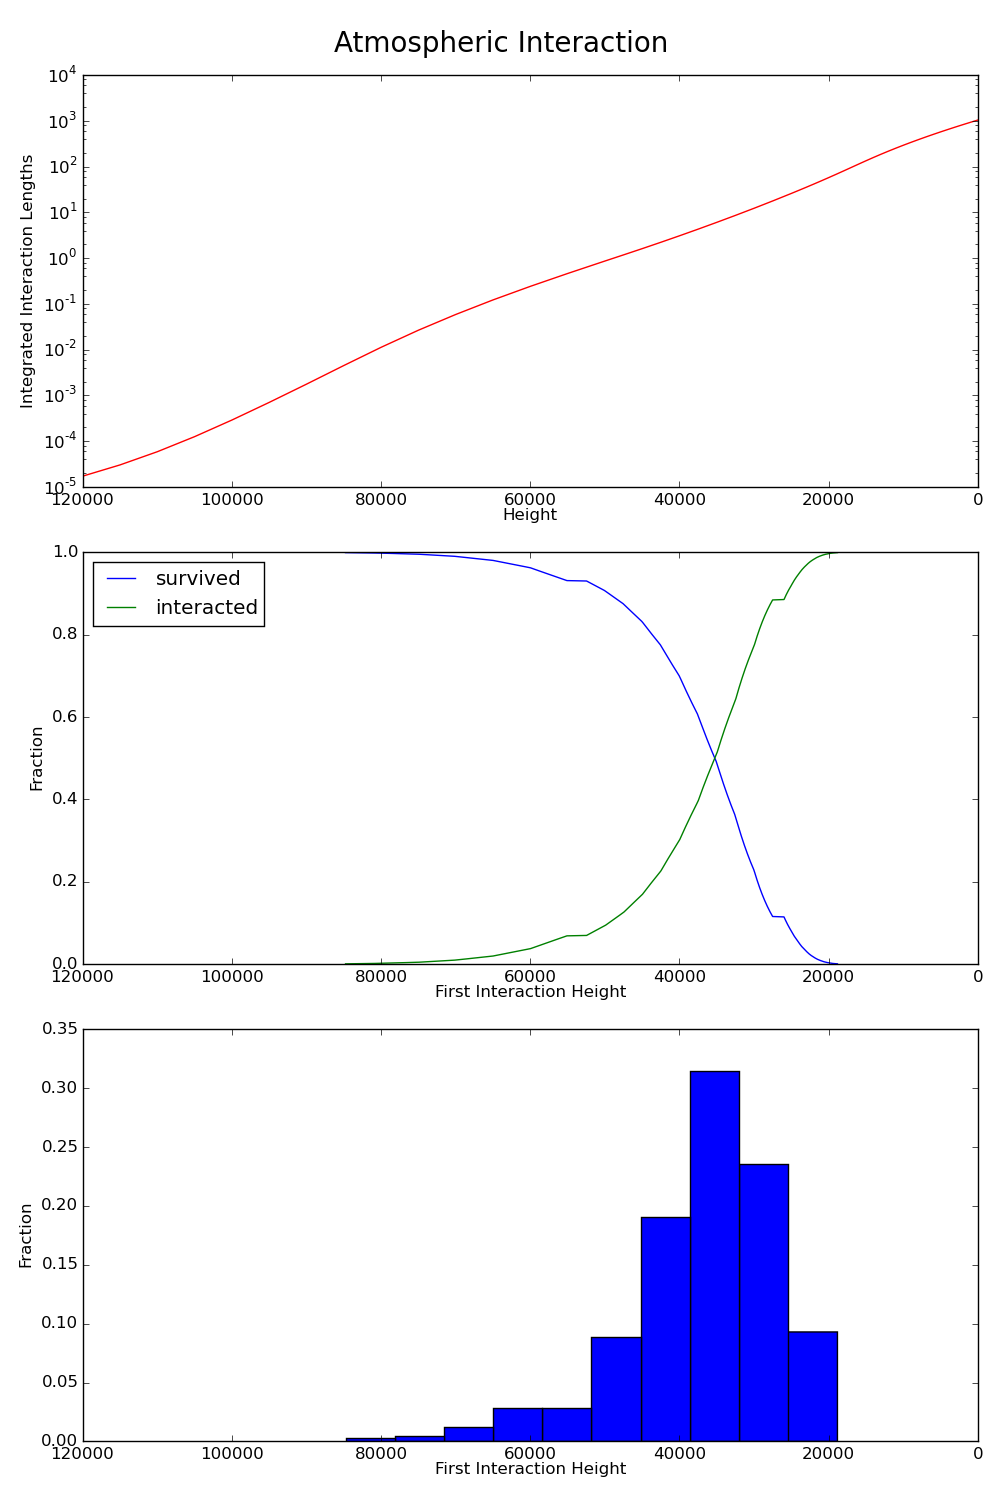
\includegraphics[height=0.9\textheight]{generalheight}
\caption{Above, the integrated interaction lengths increases as height decreases. Thus the decay probability follows a exponentially increasing distribution. In the centre, the survival and decay fractions are illustrated as a function of height. The median occurs around 40km, where the two lines intersect. Below, the fraction of interacting particles in each height band is shown in a histogram. The mean first interaction height for all events is roughly 40km above sea level.}
\label{fig:generalheight}
\end{center}
\end{figure}

To simulate the First Interaction Height, we assign a uniform random number R to each event, corresponding to the $P_{survival}$ at which the cosmic ray will interact. R can be interpreted fraction of events that will have interacted before the simulated cosmic ray does. It ranges from R=0 for interaction at the top of the Atmosphere to R=1 for an event reaching the ground. Having determined the fraction of events, we assume the survival probability is normalised. As with all exponential distributions, we see that the expectation value is equal to one Interaction Length.

\[ P_{survival}(x) = k e^{\frac{-x}{x_{0}}} \Longrightarrow \int_{0}^{\infty} P_{survival}(x) dx = k x_{0} [ e^{0} - e ^ {- \infty}] = 1 \Longrightarrow k = \frac{1}{x_{0}}\]
\[P_{half}(x) =\int_{0}^{x_{median}} k e^{\frac{-x}{x_{0}}} dx =[1 -e^{\frac{-x_{median}}{x_{0}}} ]= \frac{1}{2} \Longrightarrow {x_{median}} = x_{0} \ln (2)\]

\[ <x> =  \int_{0}^{\infty} P_{survival}(x) dx = x_{0} = \frac{x_{median}}{\ln (2)} \]

Thus, we can simply calculate $x_{0}$ as the expectation value of interaction length. This parameter is free-floating, and can only be determined through experimental study of Cosmic Rays. Experimental results indicate an approximate cross section of $\sigma_{Fe-air} = 2000mb$ and thus a corresponding value of $x_{0} \approx 12 g cm^{-2}$ \cite{Montanus2013}. 

As with energy, we wish to simulate a realistic spectrum for the first interaction heights. We must thus convert the uniform random number R to an interaction distance X. Using the standard atmospheric tables, the corresponding height value can be found using exponential interpolation. The standard atmospheric data is included in the appendix.

\[ R = \int_{0}^{X} k e^{\frac{-x}{x_{0}}} dx = [1 -e^{\frac{-X}{x_{0}}}] \Longrightarrow X = -x_{0} \ln (1 - R) \] 

Interpolating the value of the height neglects the fact that some cosmic rays which would not interact with the atmosphere before reaching the ground. The integrated interaction lengths are equal to about 850 at an altitude comparable to the HESS site. There is thus a probability of reaching the ground equal to $P = exp(\frac{-850}{12}) \approx 1.73 \times 10 ^{-31}$. It is thus reasonable to ignore this tiny fraction of events, and instead assume that every cosmic ray will interact at some point in the atmosphere.

As cited by the HESS study, a typical first interaction height is roughly 30km for a Cherenkov-Emitting event \cite{hess07}. With the assumed value of $x_{0}$, a simulation was conducted to determine the expected interaction heights for Cosmic Rays. It is found that the mean first interaction height of 36.9km and a median first interaction height of 35.2km for all cosmic rays. However, when Cherenkov-Emitting events are considered, we have both a median and mean first interaction height of 30.3km, which clearly agrees with our expectations. Considering solely high-multiplicity events, we find that these have a mean height of $h \approx 23 \pm 5$ km, as shown in Figure \ref{fig:Hessheight}.

\begin{figure}
\begin{center}
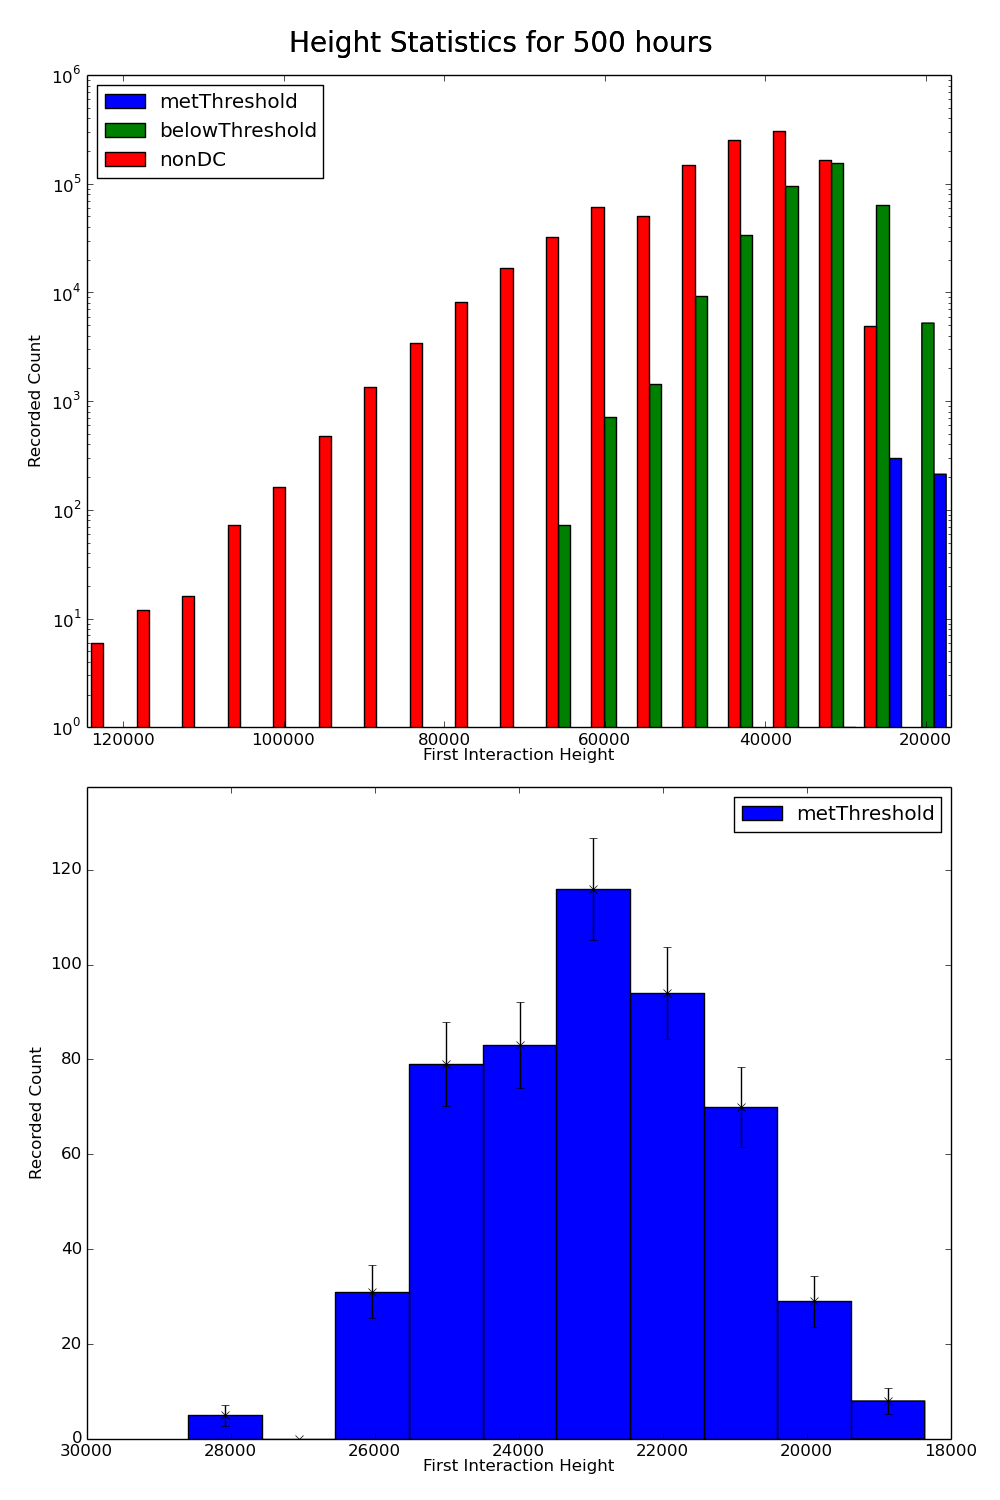
\includegraphics[height=0.9\textheight]{hessheight}
\caption{The mean first interaction height for all Cherenkov Events is 40km. Events in blue met the multiplicity threshold, with DC light in four telescopes. The mean first interaction height for all Cherenkov events is 30km, while for high-multiplicity events in the HESS array it is 23km.}
\label{fig:Hessheight}
\end{center}
\end{figure}

Another parameter that could be modelled is $\tau$, the optical depth to the surface. The Cherenkov Light, mostly emitted in the visible blue part of the EM spectrum, experiences relatively little atmospheric absorption. The major component of Rayleigh-scattering-based atmospheric absorption occurs in the lower part of the troposphere, and thus the atmospheric absorption is almost independent of emission up to first interaction height. For a given emitted intensity $I_{0}$ we find that the corresponding I received on the ground decays exponentially with optical depth, so that $\frac{I}{I_{0}}=e^{-\tau}$ with $\tau=\int_{0}^{l}ds$. However, the CORSIKA parameterisation has already accounted for any influence of atmospheric absorption. It is likely that this, in part, contributed to the value of $\sigma_{DCrgr}$.

\subsection{Full-Shower event reconstruction}
The full shower image amplitude seen in a telescope depends on the core position and the core energy. We have determined a very clear parameterisation of this LPD, along with the expected LPD fractional deviation of $\frac{\sigma_{I}}{I}= 0.15$. The received full shower amplitude is simulated under the assumption of a Gaussian distribution around the expected value. We can thus reconstruct the core position and energy using a Log Likelihood minimisation. Once a Cosmic Ray has reached saturation, the Cherenkov Emission is effectively independent of its energy, barring determination of the first interaction height. Consequently, the energy value is solely determined by the full-shower amplitudes. 

Having observed the full shower in n telescopes out of five, we consider each of the total photoelectron counts $N_{i, received}$. We aim to determine the expectation value of the LPD, $\mu(x, y, Energy$) , which led to the measurement $N_{i, received}$. For a given expectation value, we know the corresponding probability of observing $N_{i, received}$ will be the standard Gaussian probability, with a sigma of $\sigma = 0.15 \times \mu$.

\[  P_{i} ( N_{i, Received} \mid X, Y, Energy )  =  \frac{1}{\sqrt{2 \sigma^{2} \pi}} \exp(-\frac{(N_{i, Received} - \mu)^{2}}{2 \sigma^{2}}) \]

To reconstruct the event parameters, we must minimise the probability of a given set of observations. We know that the probability of obtaining a set $N_{i,received}$ will simply be the product of the probability of each individual measurement, $\mathbb{P}(x, y, Energy) = \prod_{i=1}^{n} P_{i}(x, y, Energy)$. For convenience we minimise the negative log likelihood instead, in which case we find that we can sum over the contribution of each telescope. We then minimise the function by varying the core position and energy, to find the most likely values for those parameters.

\[ - \ln(L) = - \sum_{i=1}^{n} \ln(P_{i}) =  \sum_{i=1}^{n} [ \frac{1}{2}\ln(2 \pi) + \ln(\sigma) + \frac{(N_{i, Received} - \mu)^{2}}{2 \sigma^{2}}]\]

The minimsation is done with the iMinuit python package, which calls the MINUIT algorithm to seek a minima in a multi-dimensional parameter space \cite{James75}. Due to the discontinuous nature of the likelihood function in the case of non-observation of an air shower, it is sometimes the case that the MINUIT algorithm will find a local rather than global minima. To mitigate this problem, we can start the minimisation on points in a lattice of starting values within the parameter space. In each case, we would find a local minimum and an assosiated likelihood. We can then select the local minimum with the smallest associated likelihood as the global minimum for the entire parameter space. 

Using basic Hillas reconstruction techniques we can find a rough estimate of the core position. For each telescope, we will obtain an expected direction to shower core, although it will be heavily Gaussian-smeared from the true direction. However, combining these values can restrict us to an expected target region. We consider a grid of spacing 5m in the xy plane, and with each telescope, consider the reconstructed direction to shower core. Allowing a certain angular deviation will give us a target region containing certain likely grid points. We progressively increase the angular deviation until we have found the twenty most likely core position points. It is important to note that these core positions are simply starting points for a minimisation. The minimisation itself is allowed to float freely anywhere in the simulated target grid of $300 \times 300 = 90000 m^{2}$.

In addition, with reference to the energy power law, we consider 50 starting energy values. We again use the energy range 35-135 TeV, and as with the initial simulation of the core energy, we convert probabilities to energys. In this case, the probability range 0-1 is split into 50 evenly-spaced values, and each of these is converted into a corresponding energy coordinate. Thus most of the energy values are found at the lower end of the spectrum, because this is also where the true values for most events will be found.

In combination, we consequently have a total of 1000 minimisations. Having run the minimisation algorithm, we thus acheive a full-shower LPD reconstruction, and obtain a measurement of the core energy and starting position. The resulting fraction error in energy distribution is shown below in Figure \ref{fig:rawepn}. Under the assumption of a gaussian distribution, we can calculate the mean fractional deviation as half of the distance between the 16th and 84th centiles of data. We sort each fractional deviation, and expect that 68\% of events will lie between these values. Using this method, it is clear that the energy reconstruction is fairly good, with a fractional standard deviation of roughly 0.10 when both four and five telescope events are considered. Having now reconstructed the value of the energy with reasonable accuracy, we can make use of this value when attempting to reconstruct the DC LPD. 

\begin{figure}
\begin{center}
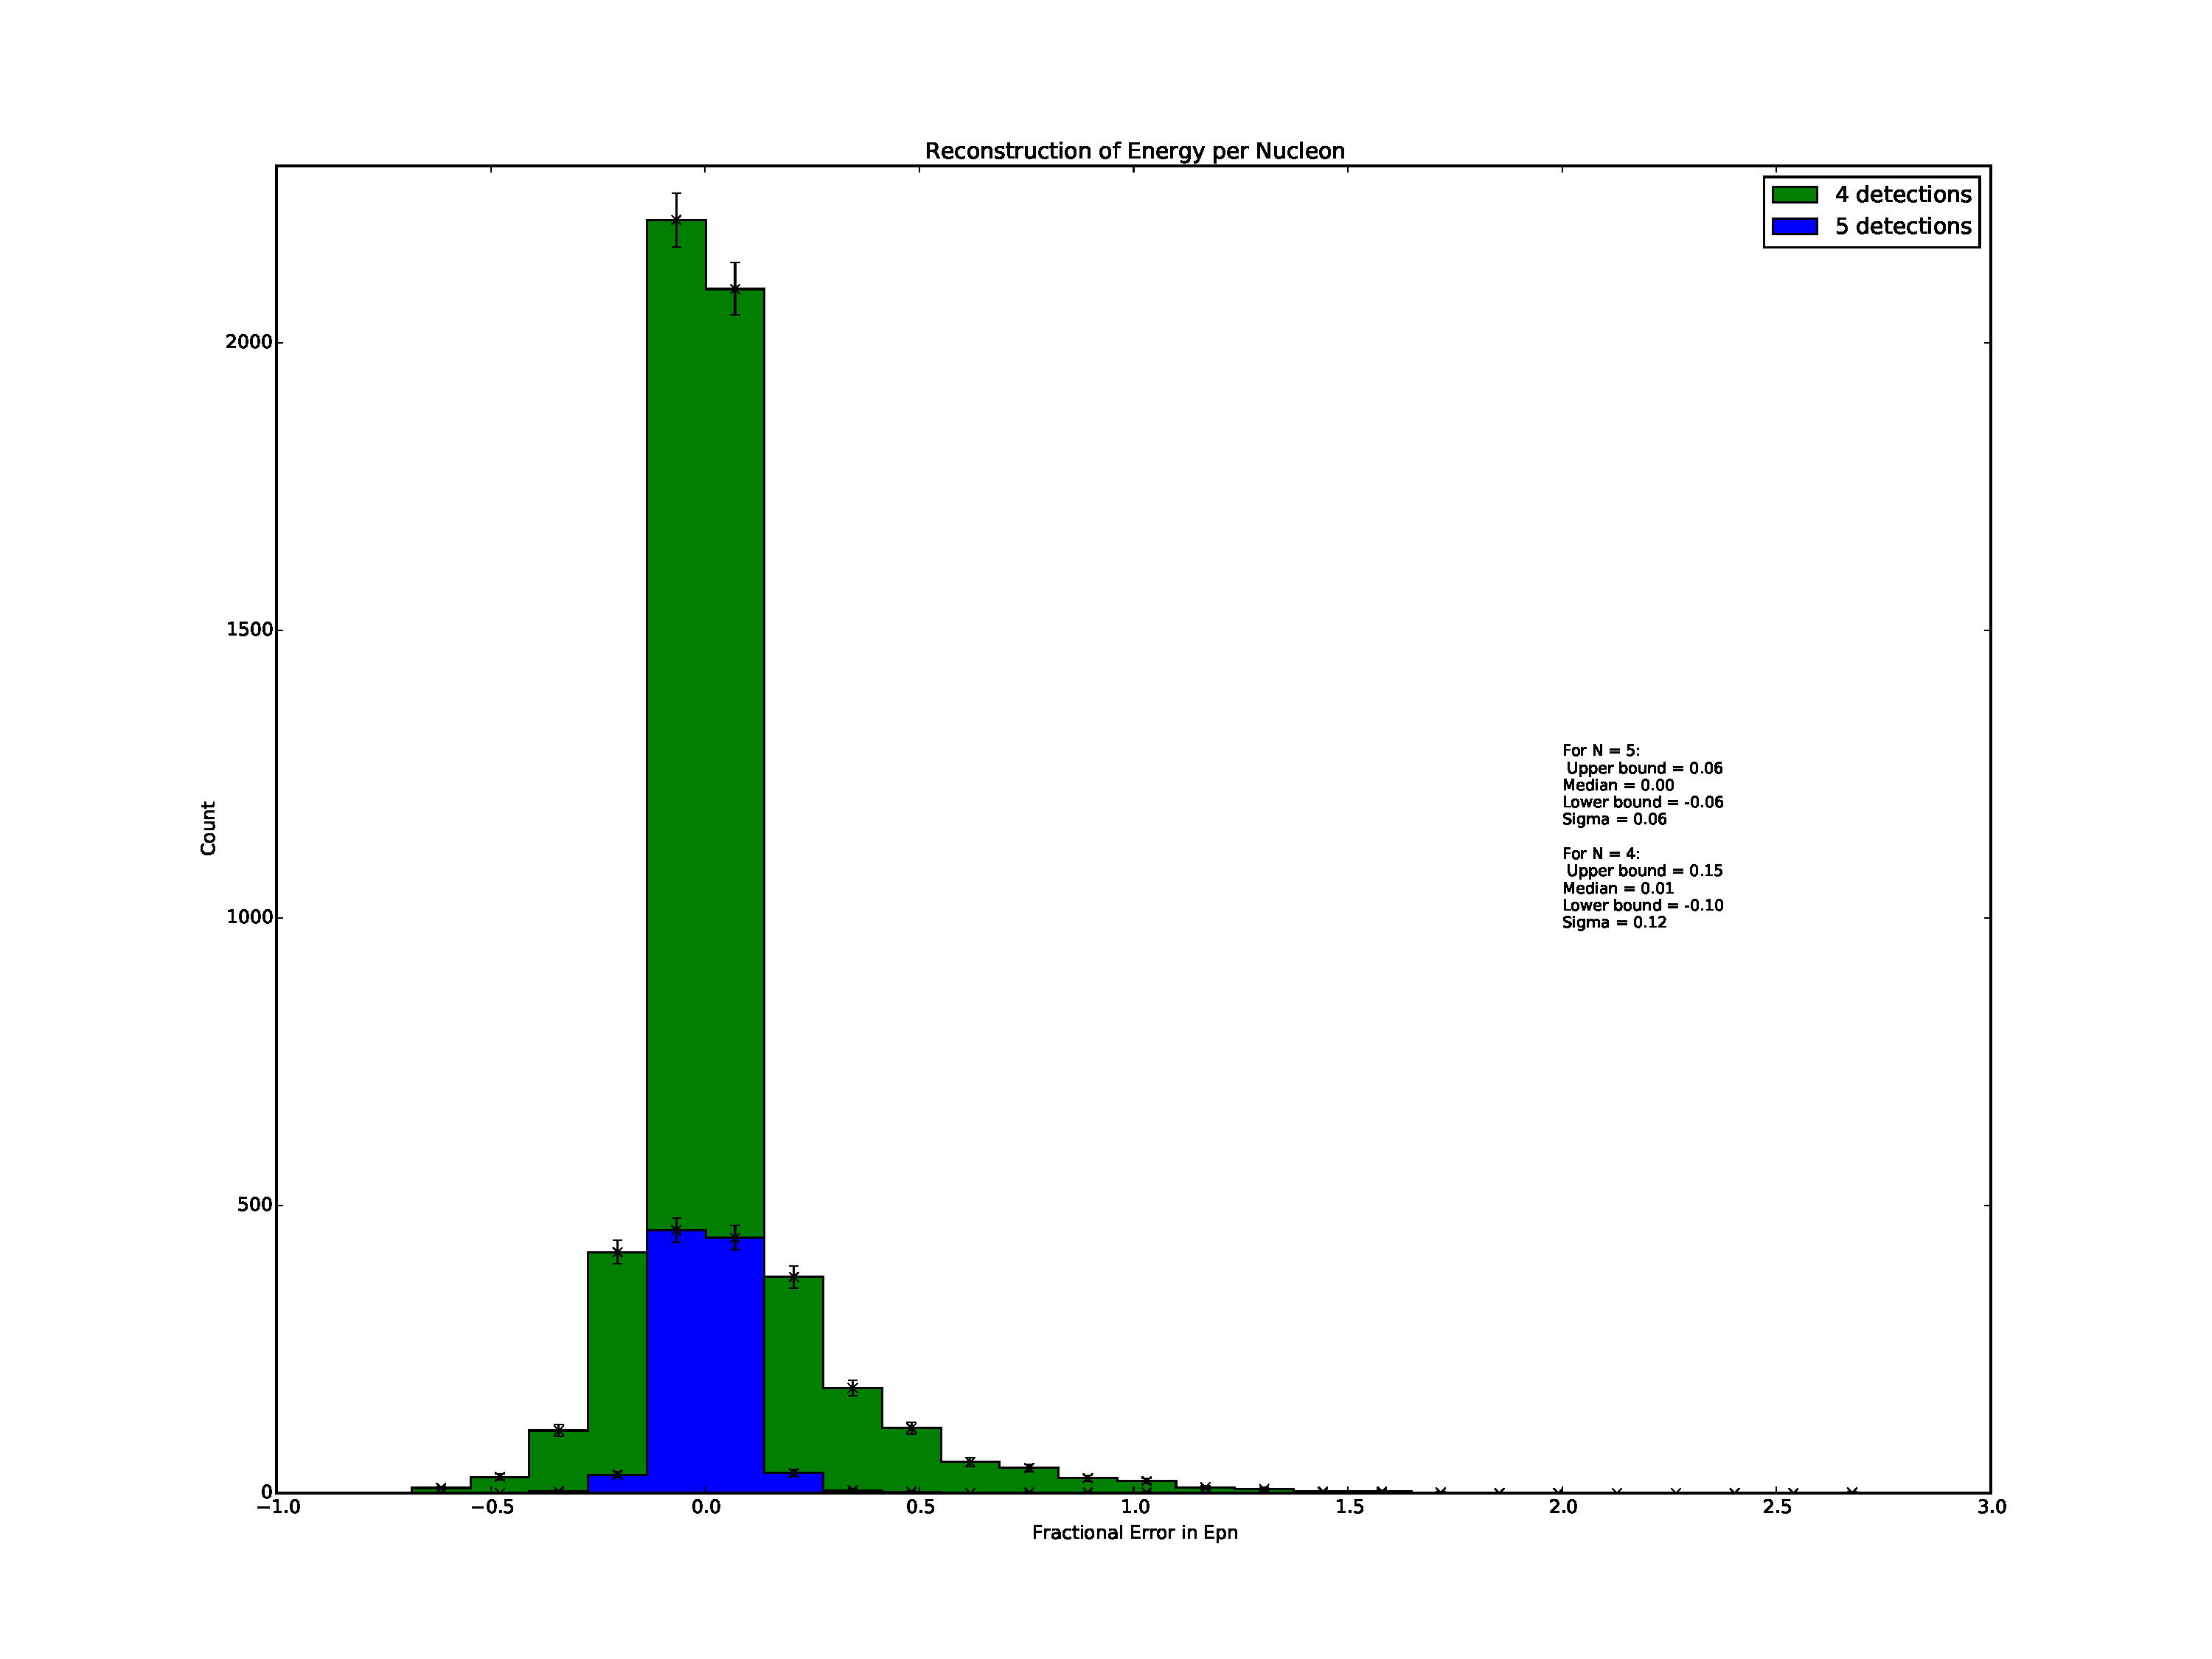
\includegraphics[width=\textwidth]{rawepn}
\caption{The fraction deviation from true energy is shown above. For events with five-telescope multiplicity, the fractional error is 0.06 but for four-telescope multiplicity, it is 0.12. The expected poissonian error bars are also shown.}
\label{fig:rawepn}
\end{center}
\end{figure}

A graph showing the difference between the distance from telescope to true core position, and the distance from telescope to this reconstructed core position. Using the same 68\% method, the standard deviation from the true core distance  is 10m for 5 telescope events, and 16m for four telescope events. A better estimate for the core position will take into account the DC LPD as well as the full LPD.

\begin{figure}
\begin{center}
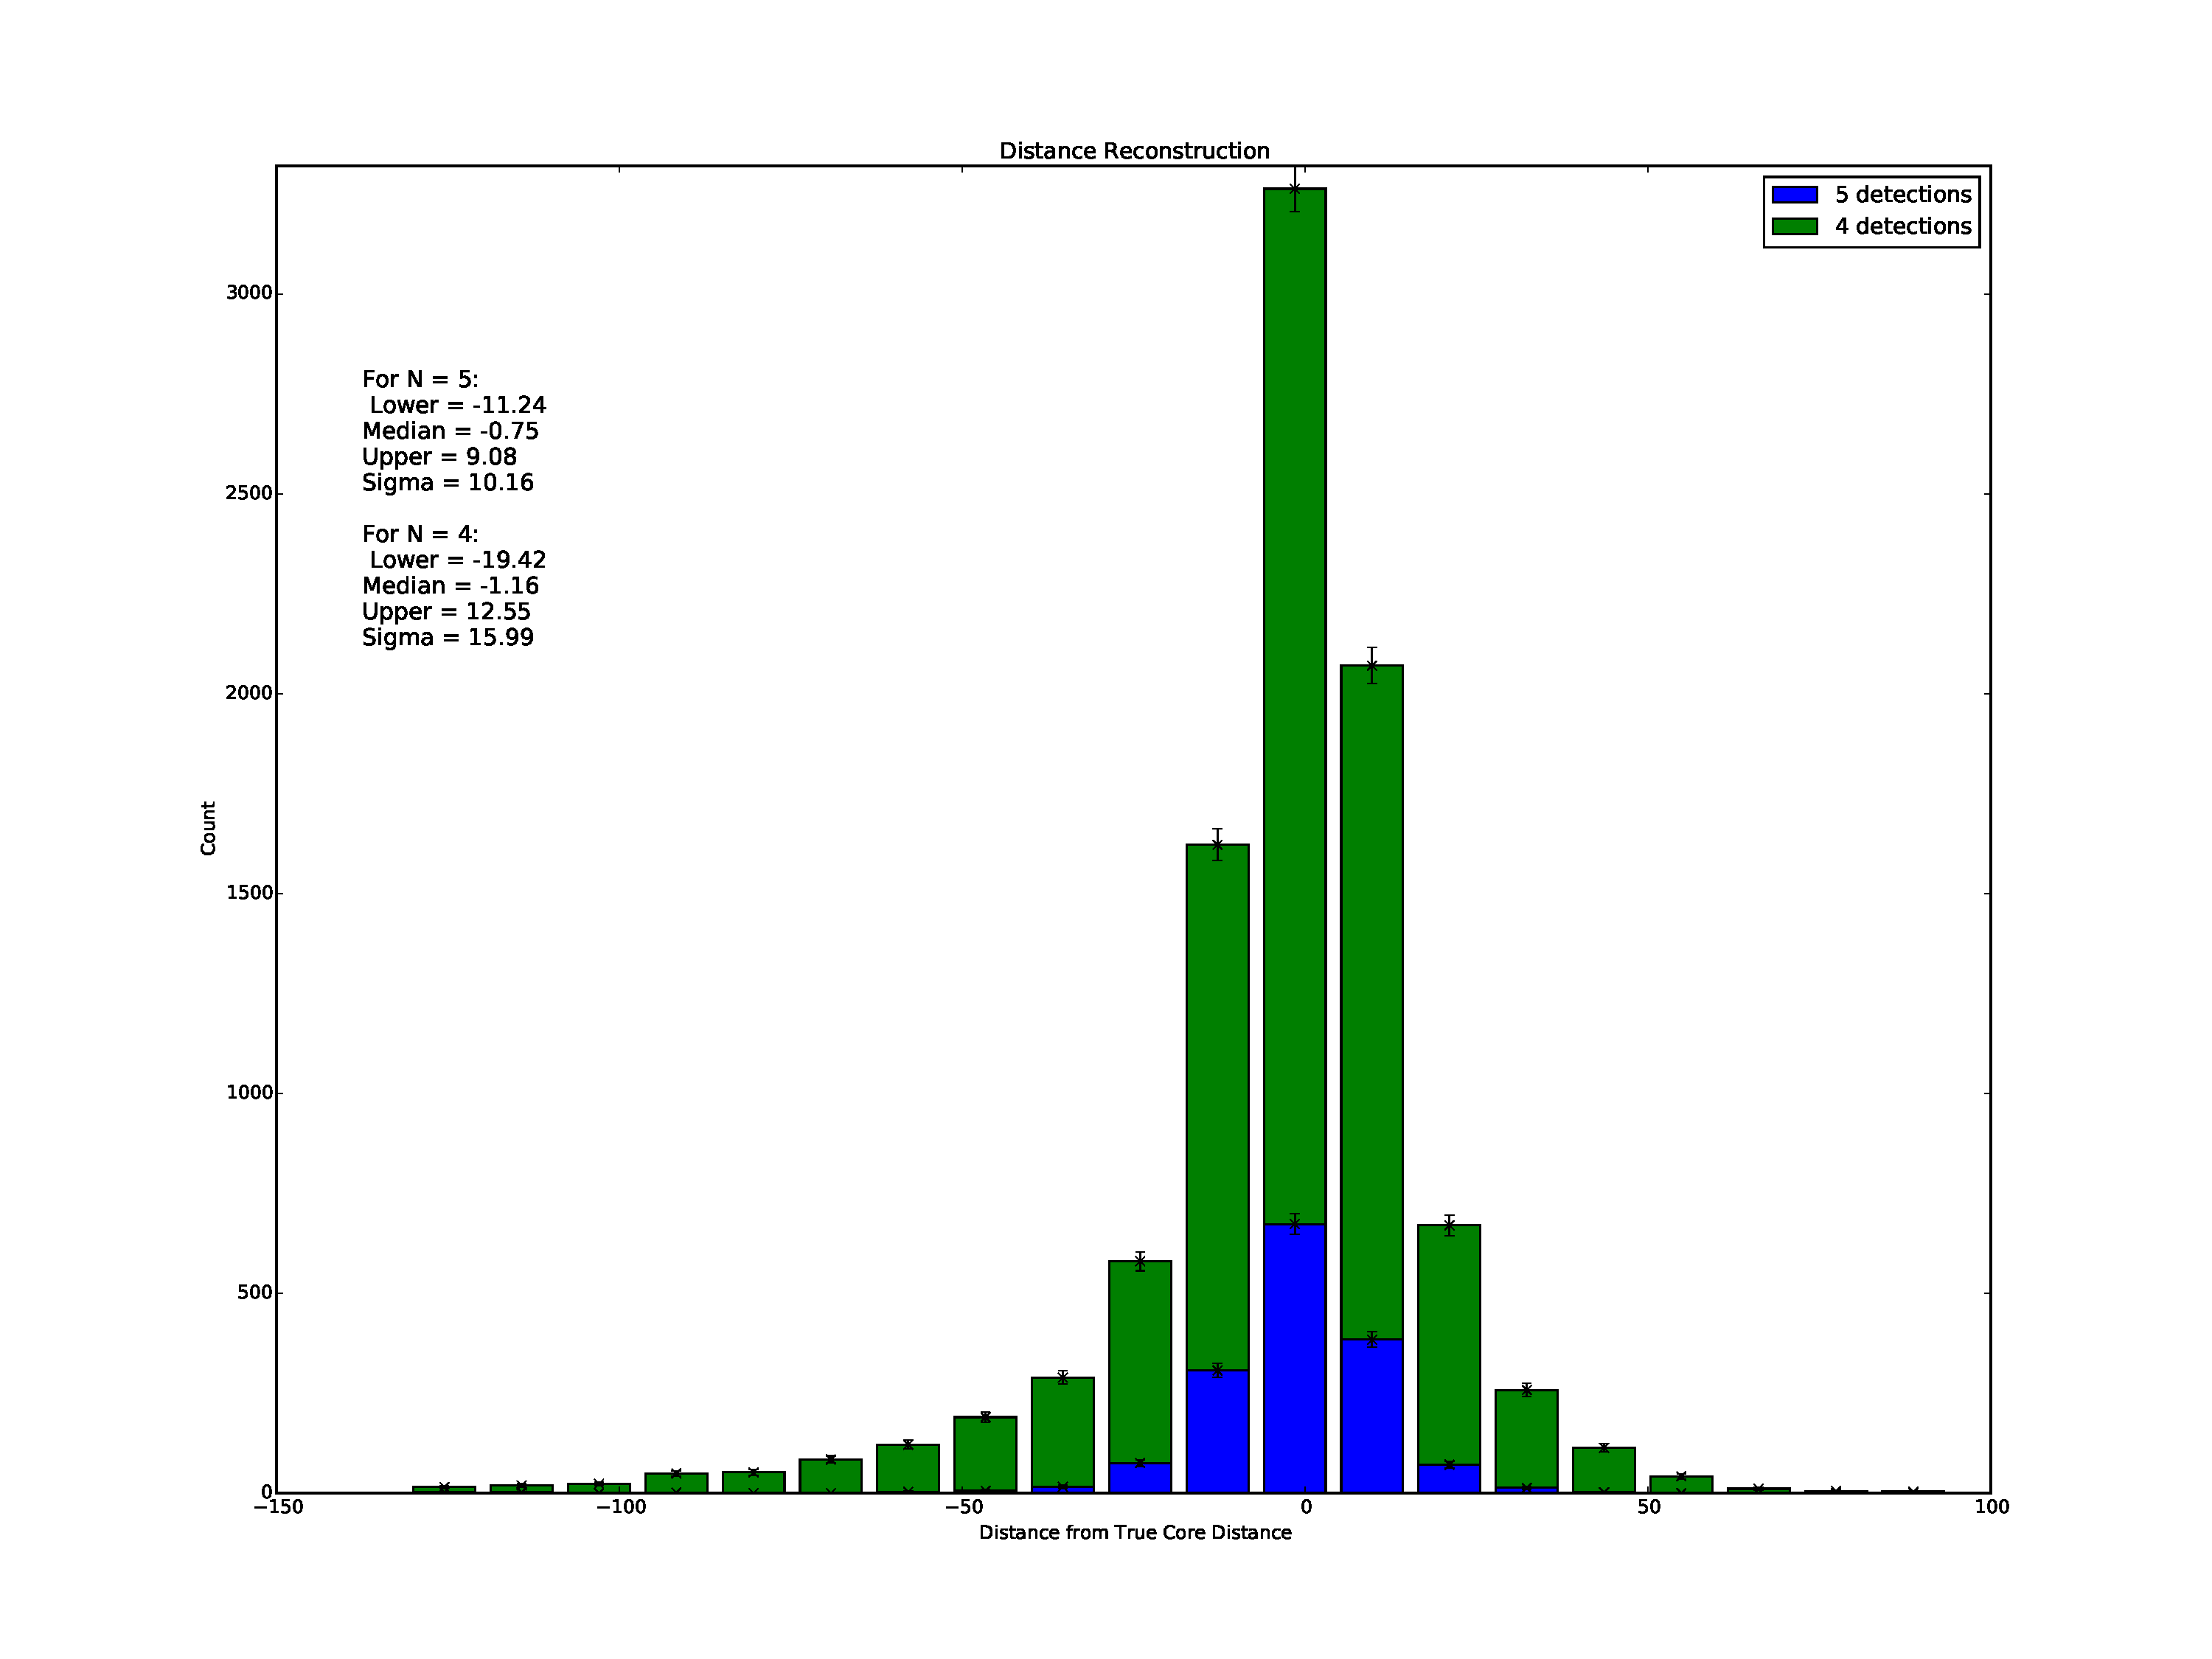
\includegraphics[width=\textwidth]{rawcoredistance}
\caption{The distance from true core to the core reconstructed with the full-LPD is shown above. For 4-tel events the standard deviation from true core distance is 16.4m while for 5-tel events, it is 9.7m.}
\label{fig:rawcoredistance}
\end{center}
\end{figure} 

It is interesting to note that, for both variables, 5-telescope events have a lower deviation that 4-telescope events. This is despite the fact that the multiplicity refers solely to the number of identified DC pixels. The number of triggered telescopes containing an air shower is almost always five for these events, regardless of whether a DC pixel exists and can be identified. We can partially explain this by considering events which are likely to have 5 DC pixels. In such a case, the core is likely to be restricted to a central ring in the region between CT5 and the outer telescopes. This relatively strong confinement reduces the potential for misreconstruction of the core position, and this indirectly improves reconstruction of the other variables.

\subsection{Log Likelihood Minimisation}
Having estimated the rough core position and energy, we would at this point use our regressor to determine the values of $candidate_{DCcount}$, based on the BDT-identified DC pixel and image parameters. Having done so, we know that these values would follow the regressor LPD. For the Monte-Carlo simulation, this step is bypassed, and the regressor LPD is instead directly simulated with a standard Gaussian smearing. Having quantified the expected deviation from the LPD under these conditions, this is a reasonable simplification that massively reduces the computing requirements for event simulation. This in turn enables us to consider a greatly expanded dataset for reconstruction attempts.
 
In order to fully reconstruct the events, we need to find the x/y core position, the Energy per Nucleon, the first interaction height and the charge. We again consider the amount of DC light that each telescope receives to be Gaussian, with an expectation of $\mu(X, Y, Z, height, Epn)$ and a standard deviation of $\sigma(\mu)$. Ultimately the energy dependence of the LPD is almost negligible over the energy range, because variable $r_{max}$ is only weakly dependent on the energy. It thus makes little sense to attempt to reconstruct the energy a second time, when we would expect no discernible improvement over the reconstruction solely based on the Full Shower LPD that was performed before. We thus fix the cosmic ray energy as that found before, and instead consider a four-dimensional minimisation in Charge, x and y core position, and first interaction height.

We then minimise the Log Likelihood function, where the total log likelihood for each telescope is equal to a sum of the full-shower LPD log likelihood and the DC LPD log likelihood. We are thus minimising a Likelihood function with nine or ten measurements from two broadly independent distributions. We consequently expect an improvement in the position reconstruction, as well as a measurement of the charge and the first interaction height.

As before, we find that the discontinuous LPD leads to a frequent identification of local rather than global minima. To overcome this problem, we can iterate over a series of starting values for the parameters, with the aim of scanning the true minimum among the many minima found. In addition to the grid of likely positions identified for the Full-Shower LPD minimisation, we can can scan the integer Z values over the range $ 20 \leq Z \leq 32 $. It should be emphasised that the charge Z is treated as a free-floating parameter during the minimisation, and is able to vary freely within the range 16-36. Similarly, three first interaction heights in the range 20-30 km are scanned, but the value is able to vary freely in the range 15-65 km. It is purely due to computer resource restraints that \textquoteleft likely coordinates' in the parameter space are scanned as a starting point for a minimisation, rather than a uniformly distributed scan. Despite the simplifications, each minimisation process will still undergo $12 \times 20 \times 3 = 720$ iterations before a final reconstruction is complete. 

\subsection{Variable Resolution}
If we compare the deviation from true core distance to each telescope, we can quantify the improvcement in core position reconstruction from minimisation based solely on the full-shower LPD. This is shown in Figure \ref{fig:coredistance}, and is directly comparable with the preliminary results in Figure \ref{fig:rawcoredistance}. As expected, the core distance resolution is reduced to 13.5m and 6.1m, which is a clear improvement over the previous measurements of core position. 

\begin{figure}
\begin{center}
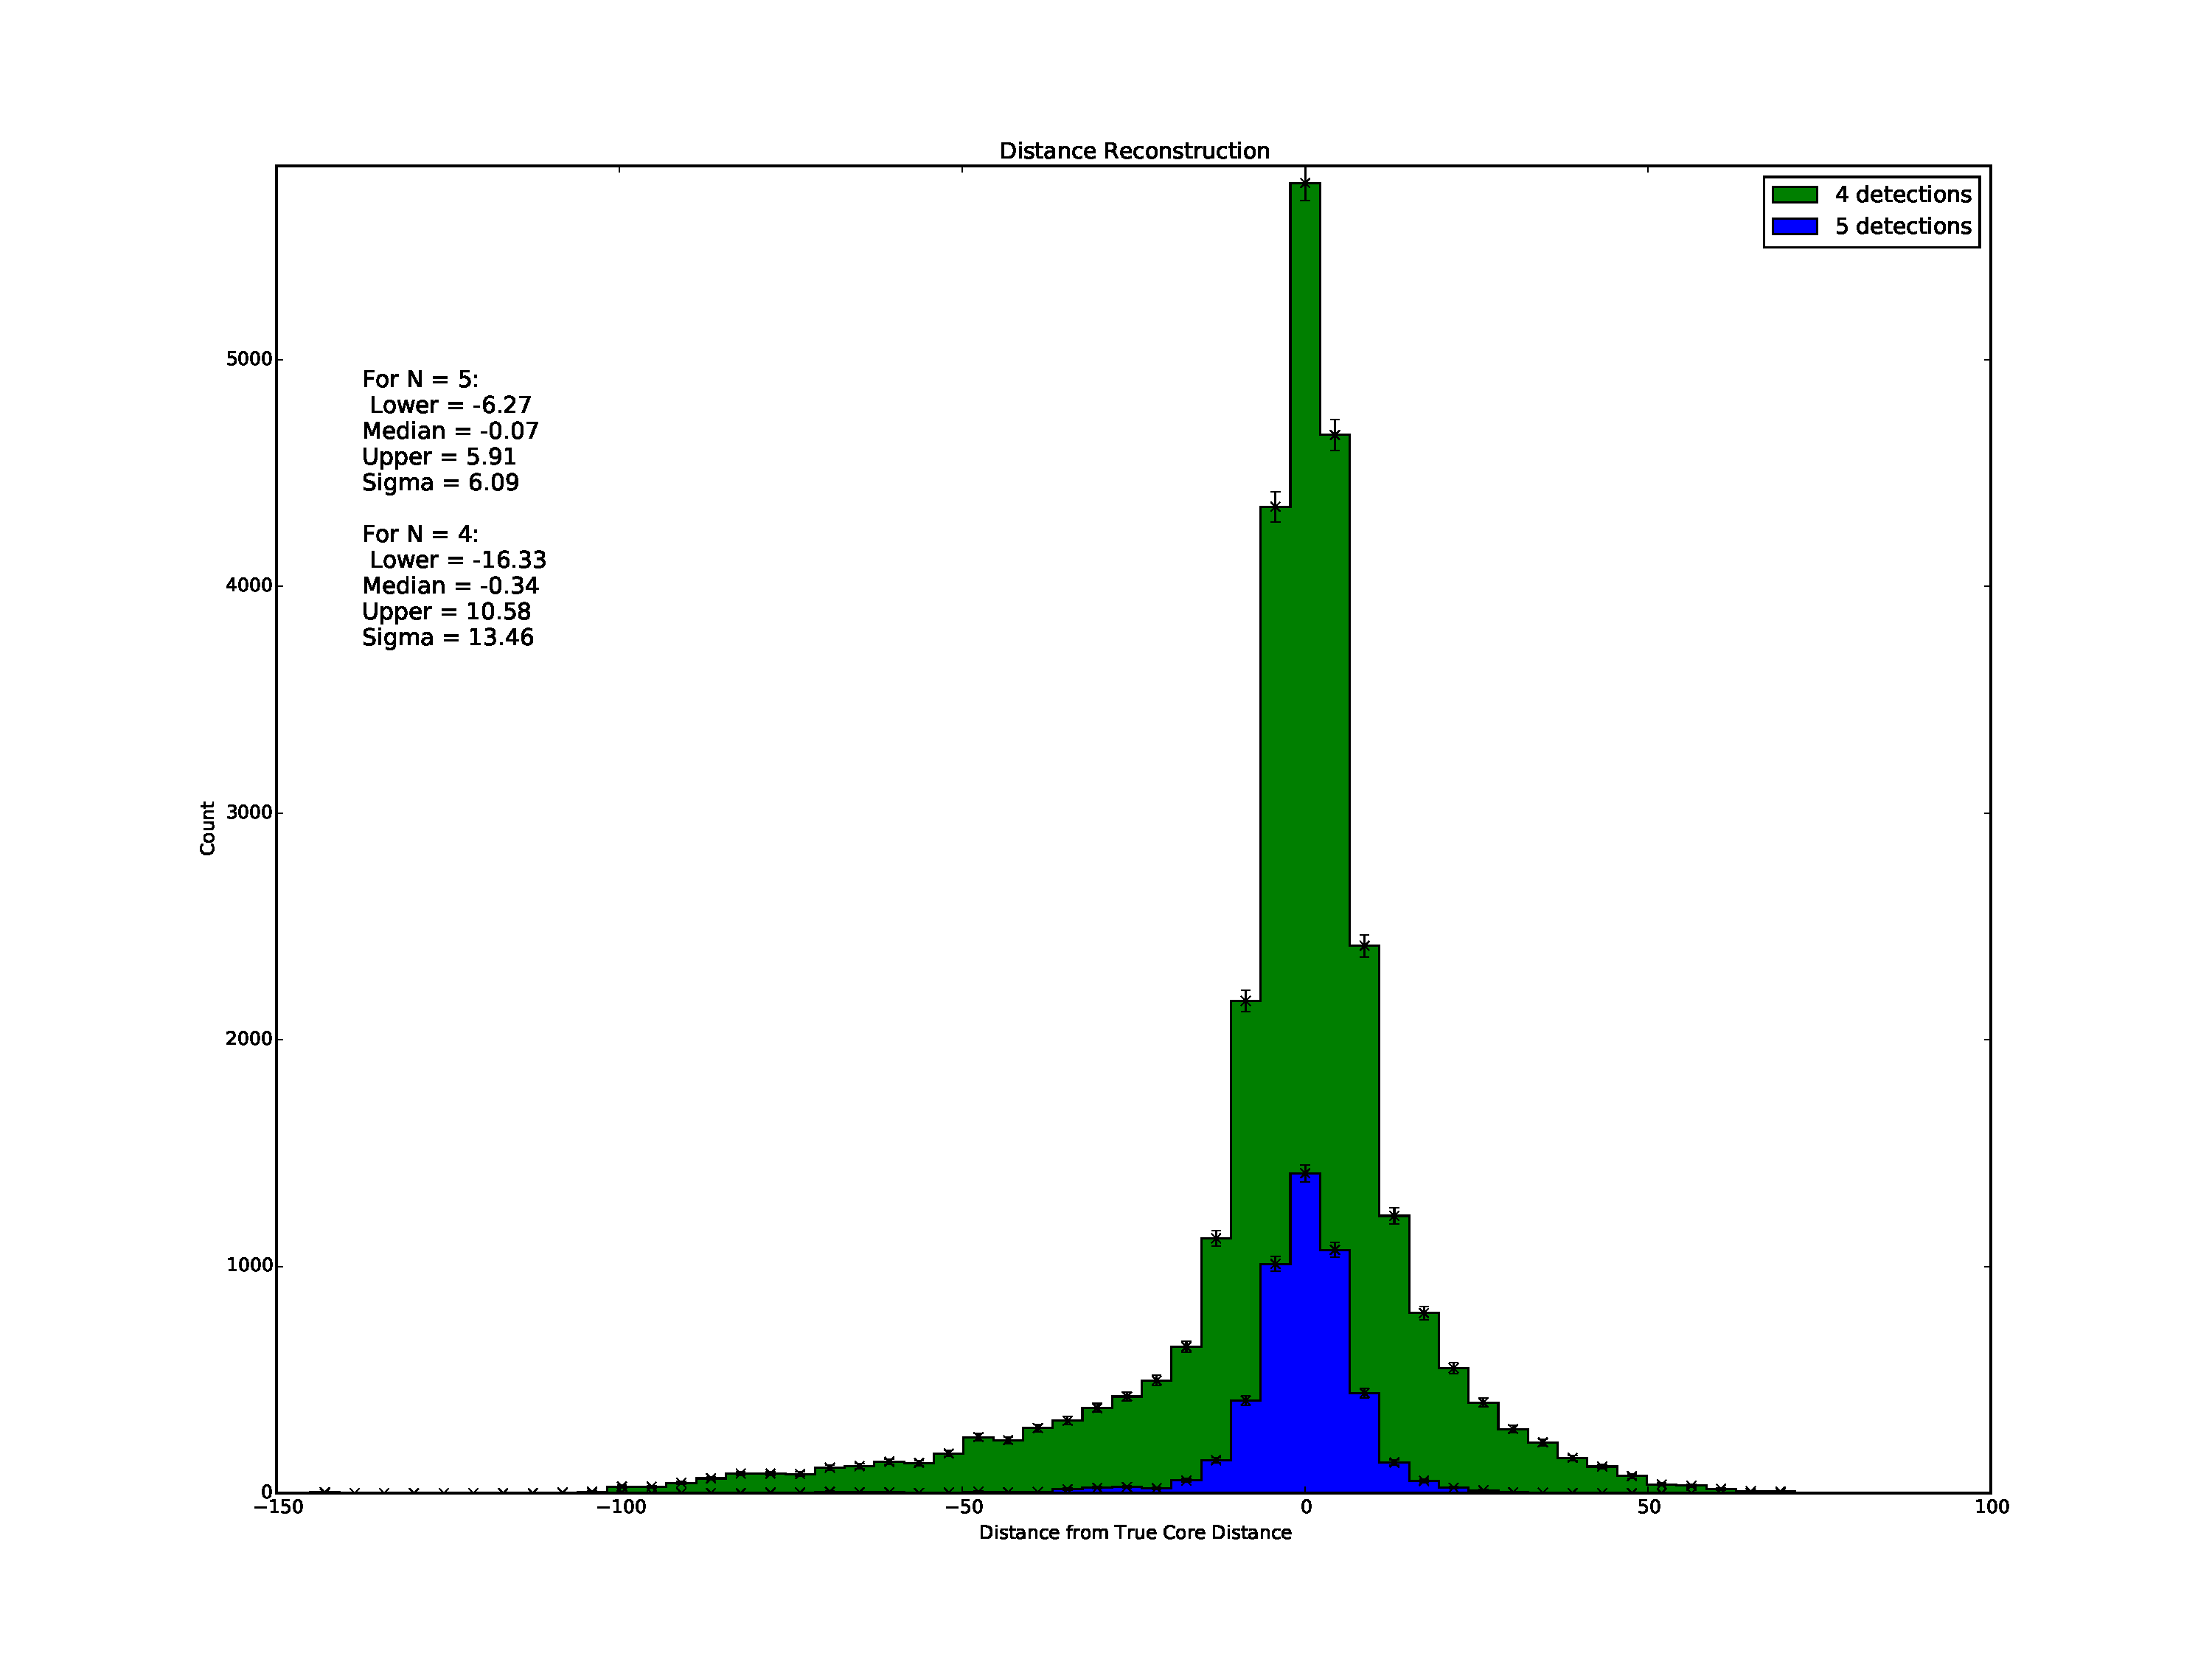
\includegraphics[width=\textwidth]{coredistance}
\caption{The distance from true core to the core reconstructed with both the full shower LPD and the DC LPD is shown above. For 4-tel events the standard deviation from true core distance is 13.5m, while for 5-tel events, it is a much smaller 6.1m. In both cases, there is clear improvement over the full-shower-only reconstruction in Figure \ref{fig:rawcoredistance}.}
\label{fig:coredistance}
\end{center}
\end{figure}

As an alternative metric for assessing reconstruction accuracy, we can calculate the absolute distance from the reconstructed core to the true core. The results of a binning of this distribution are shown in Figure \ref{fig:rawposition}. Because we consider absolute distance, this value can never be negative. Thus, we calculate a one-sided distribution standard deviation, and consider the value of an event in the 68th centile to be equal to the standard deviation. It is found that, for both four and five telescope events, the core reconstruction is approximately $\sigma_{core} = 9.1m$ and $\sigma_{core}=17.0m$ respectively. Considered together, we conclude that most high-multiplicity reconstructed core positions thus lie less than 15m from the true position. This is reasonably good, especially in comparison to the Hillas Reconstruction, where a core position resolution of $\sigma_{core} \approx 20m$ is more typical.

\begin{figure}
\begin{center}
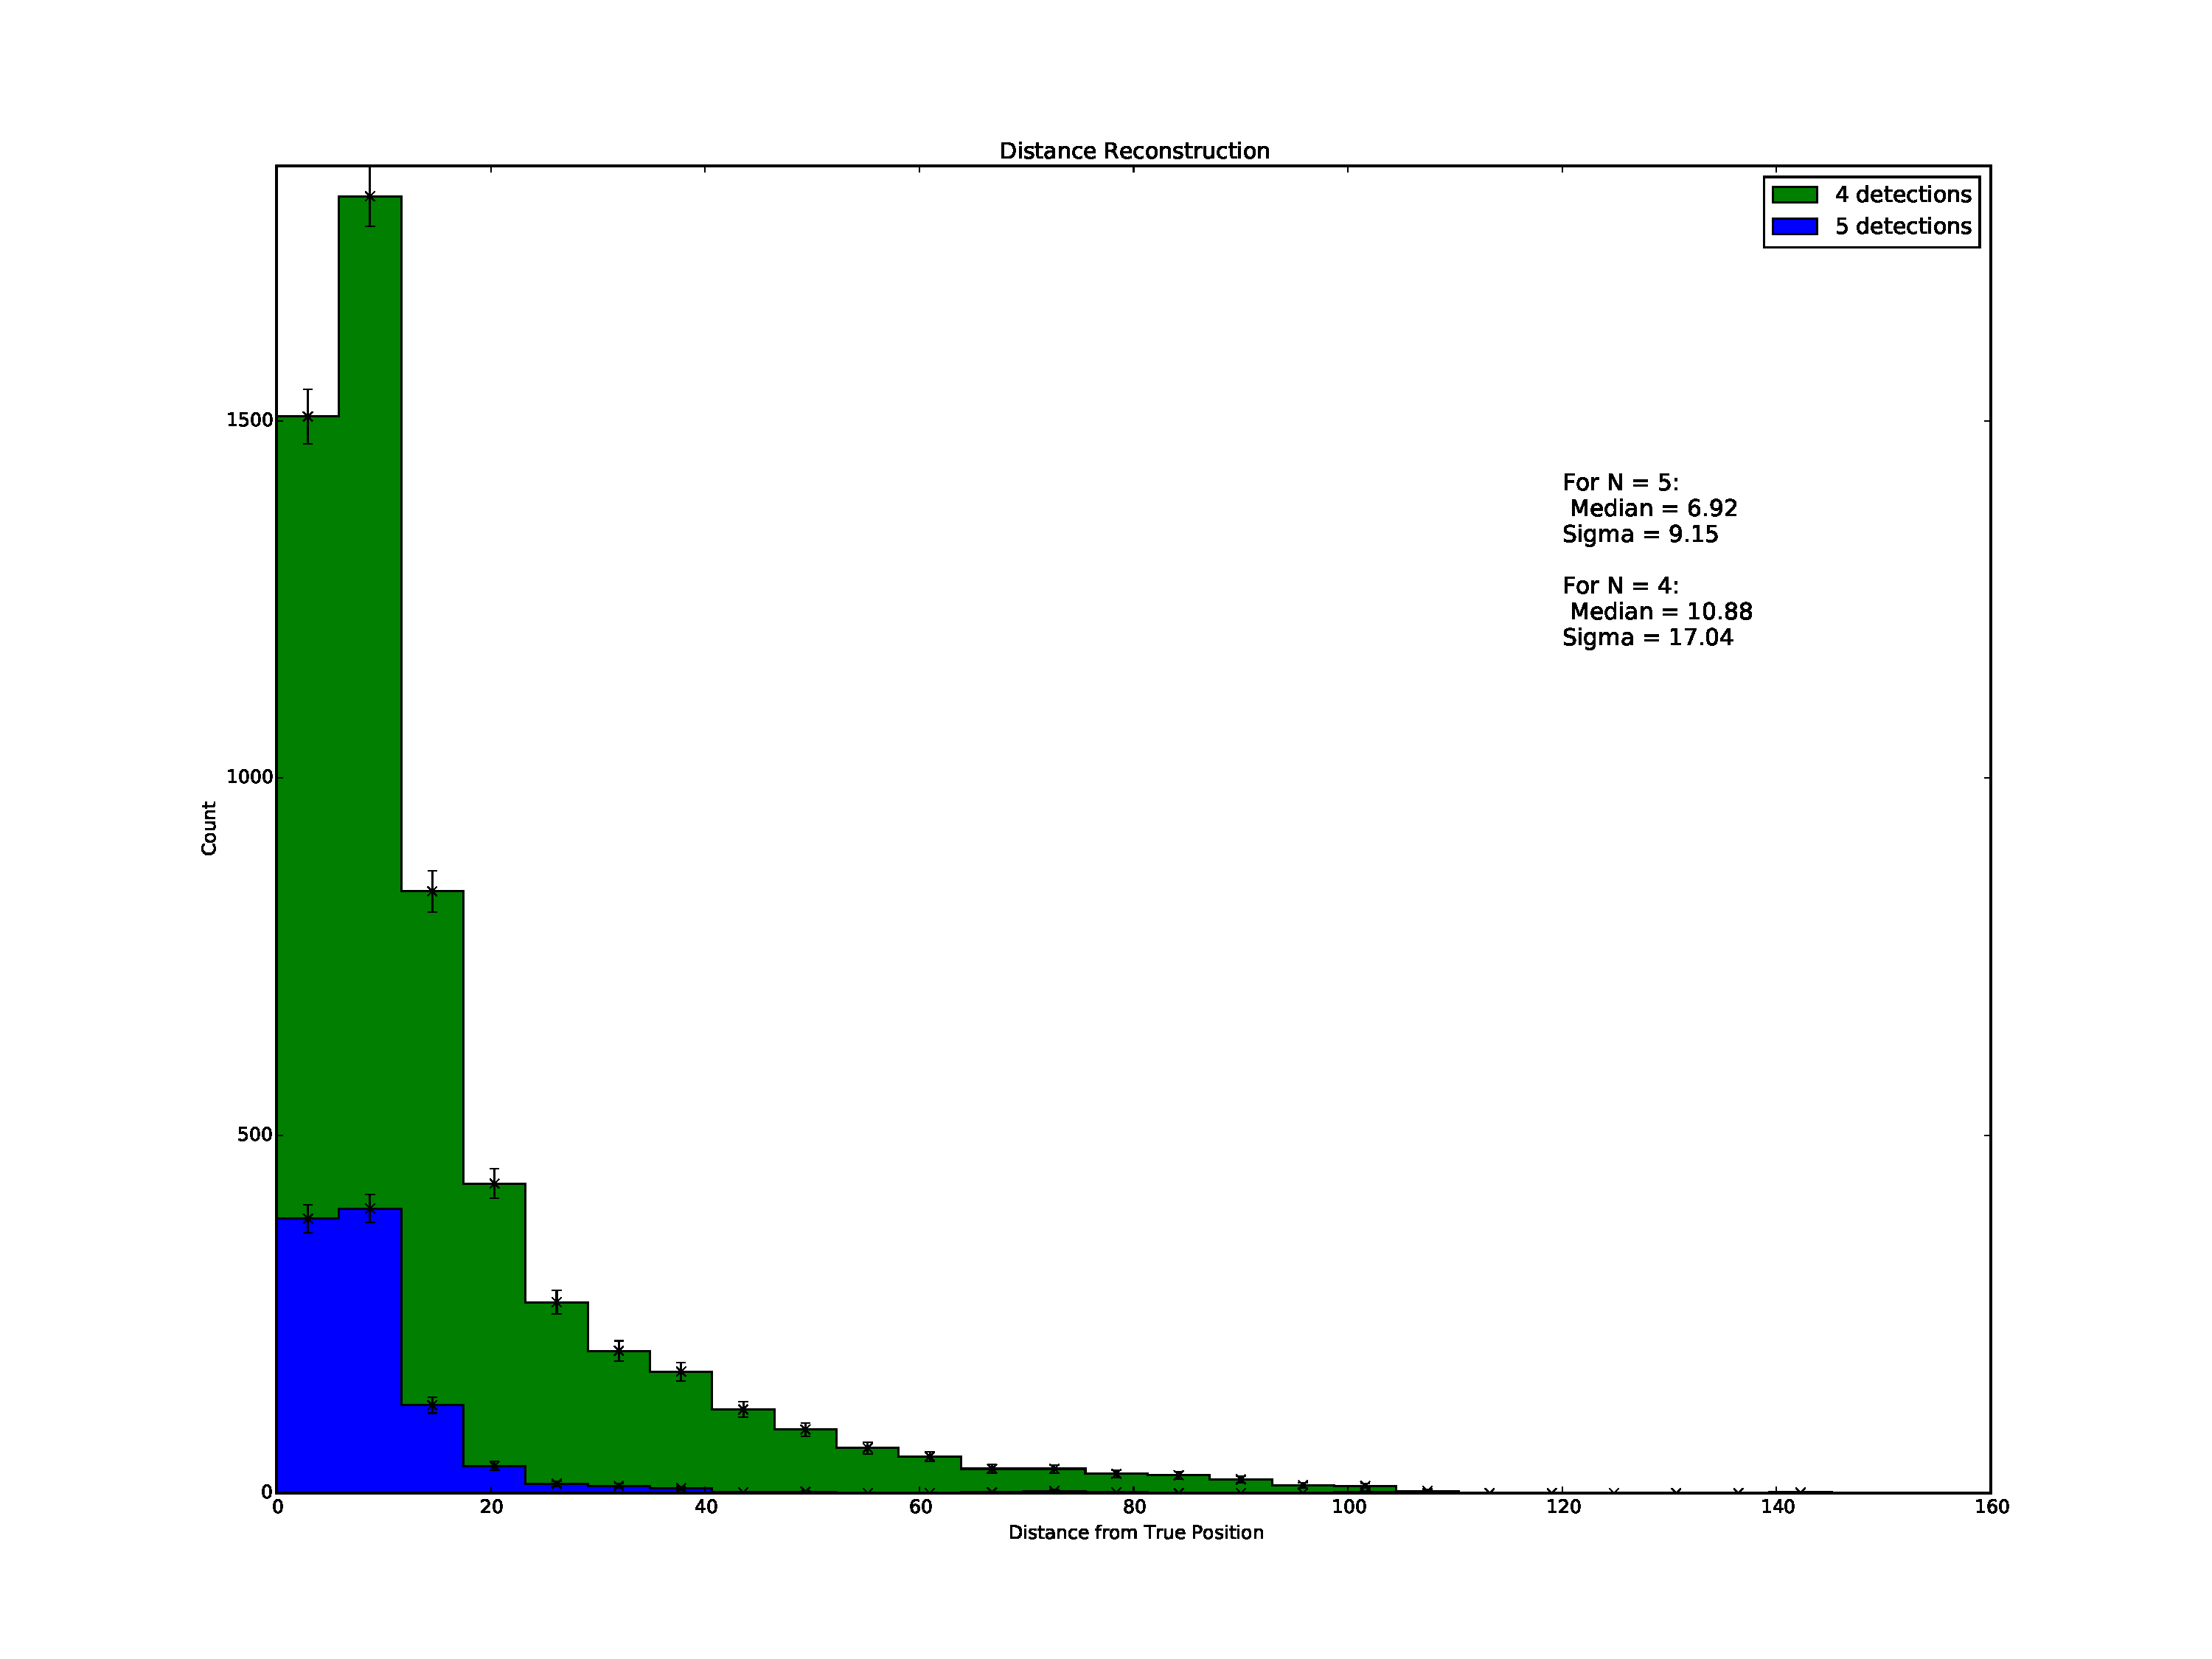
\includegraphics[width=\textwidth]{rawposition}
\caption{The distance from true core position to the reconstructed core position is shown above. For 4-tel events, the standard deviation from true position is 17.0m, while for 5-tel events, it is just 9.2m.}
\label{fig:rawposition}
\end{center}
\end{figure}

In contrast the fractional height standard deviation is of the order of 0.35. This is fairly bad but not at all unexpected, because the regressor LPD was designed to be independent of height. It is only the termination of the LPD that is height dependent, and thus it is both hard to measure but also broadly unimportant. The reconstructed height has a tendency to lie close to the starting values for height in the reconstruction process, namely 20, 25 and 30km. As seen in Figure \ref{fig:generalenergy}, the value for $r_{max}$ varies relatively little between these energies, provided that emission is saturated. On the basis of Energy cuts to remove protons, we are restricting ourselves to Energies of roughly 35TeV or more. As seen in Figures \ref{fig:lpd} and \ref{fig:generalenergy}, this is clearly sufficient for saturated emission. In fact, the extremely poor height resolution can be taken as a mark of success in that our event reconstruction is now almost completely independent of height, and therefore can't be used to reconstruct the height.  

Having taken into account our various variable uncertainties, we can also consider our most important variable. In Figure \ref{fig:rawZ} the reconstructed charge number is binned, illustrating the expected experimental results. As we would hope, there is a very clear peak centered on Z=26, and the median charge value lies very close to this value. The distributions are broadly symmetric, and have a charge resolution of $\sigma_{Z} = 1.1$ and $\sigma_{Z} = 2.2$ for five and four telescope events respectively. Unsurprisingly, the charge resolution is better for five-telescope events, but both cases represent a significant improvement over the existing charge resolution obtained through Hillas analysis. With the reasonably high event rate, we could certainly expect to see such a peak in the existing HESS data, and the uncertainty may be small enough to enable spectroscopic analysis. Obtaining such a peak is a vindication of the LPD method, and demonstrates its superior performance for event reconstruction. However, the value of $\sigma_{Z}$ for 4-telescope events is still large. It is also clear in Figure \ref{fig:rawZ} that the distribution is somewhat truncated by the imposed minimisation reconstruction range of 16-36. 

\begin{figure}
\begin{center}
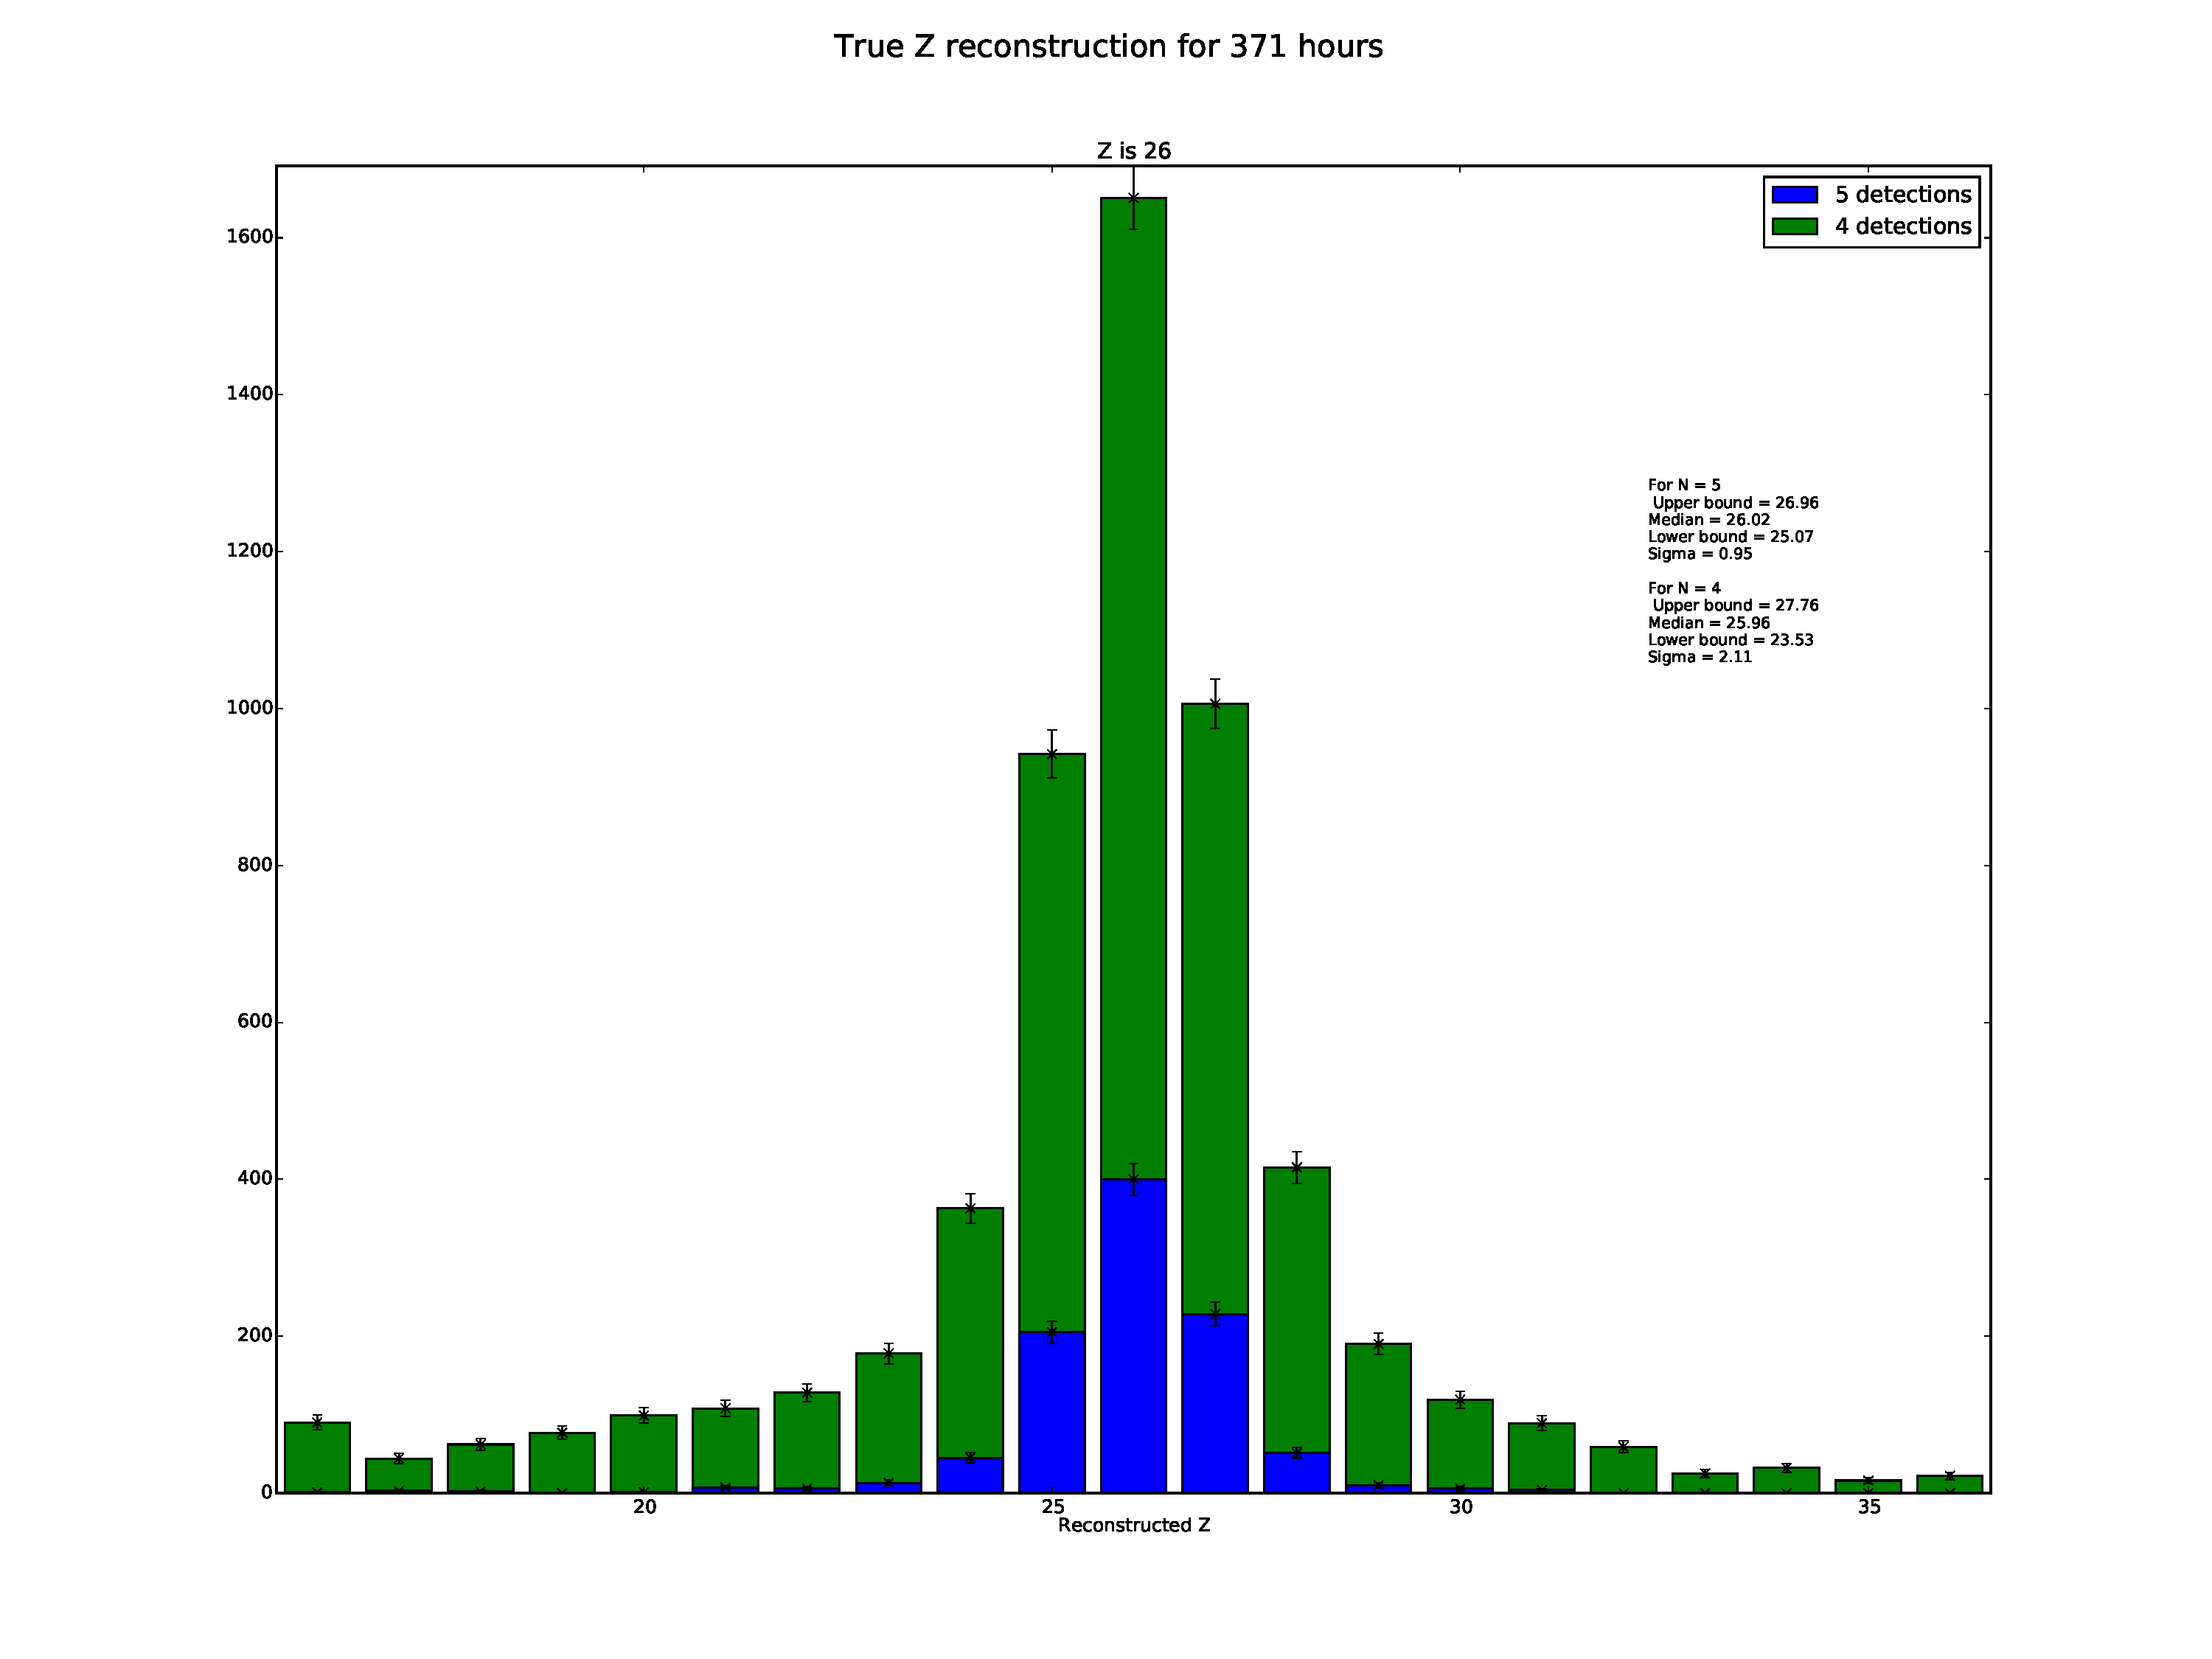
\includegraphics[width=\textwidth]{rawZ}
\caption{The reconstructed charge is shown. For 4-tel events, the median charge is 26.0 with a standard deviation of 2.1, while for 5-tel events, the median charge is 26.0 with a standard deviation of 0.95.}
\label{fig:rawZ}
\end{center}
\end{figure} 

\subsection{Boosted Decision Trees}
There is one additional possibility for improved event reconstruction. We recall that, by virtue of being a high multiplicity event, we will already be restricting ourselves to a fairly limited core position and energy range. We can train a BDT to distinguish between events that are likely to be well constructed, and those that are likely to be poorly constructed. 

Once an event has been reconstructed, we can define the expected multiplicity as the number of telescopes we would expect to see DC light in, given the reconstructed values for Energy per Nucleon, charge and core position. Using this value, alongside the core position coordinates and the energy, we train a BDT for each telescope multiplicity. Using a second set of Monte carlo data, simulated under the same conditions, we train both a 4-tel and a 5-tel BDT. The relative importance of variables is shown in table \ref{tab:reconbdt}.

\begin{table}[h!]
  \centering
  \caption{Feature Importances for the reconstruction BDTs, ordered by 4-tel importance}
  \label{tab:reconbdt}
  \begin{tabular}{ccc}
    \toprule
    Variable & 4-tel & 5-tel\\
    \midrule
    Energy per Nucleon & 0.29 & 0.30\\
    Core y Position & 0.27 & 0.31\\
    Core x Position & 0.26 & 0.31\\ 
    Expected Multiplicity & 0.19 & 0.07\\
    \bottomrule
  \end{tabular}
\end{table}

It is interesting to note that, although the energy and core position always have similar importance, the expected multiplicity is far more important for the 4-tel BDT. This implies that many poorly reconstructed events have core positions that would lead to an altered multiplicity. If a telescope is not triggered, it is currently ignored for the purpose of reconstruction. Consequently events can be reconstructed with core positions that we know to be false. We apply each BDT to the Monte Carlo data with matching multiplicity, to identify events that are likely to be reconstructed. The BDT score distribution is shown in Figure \ref{fig:reconBDTdistribution}.

\begin{figure}
\begin{center}
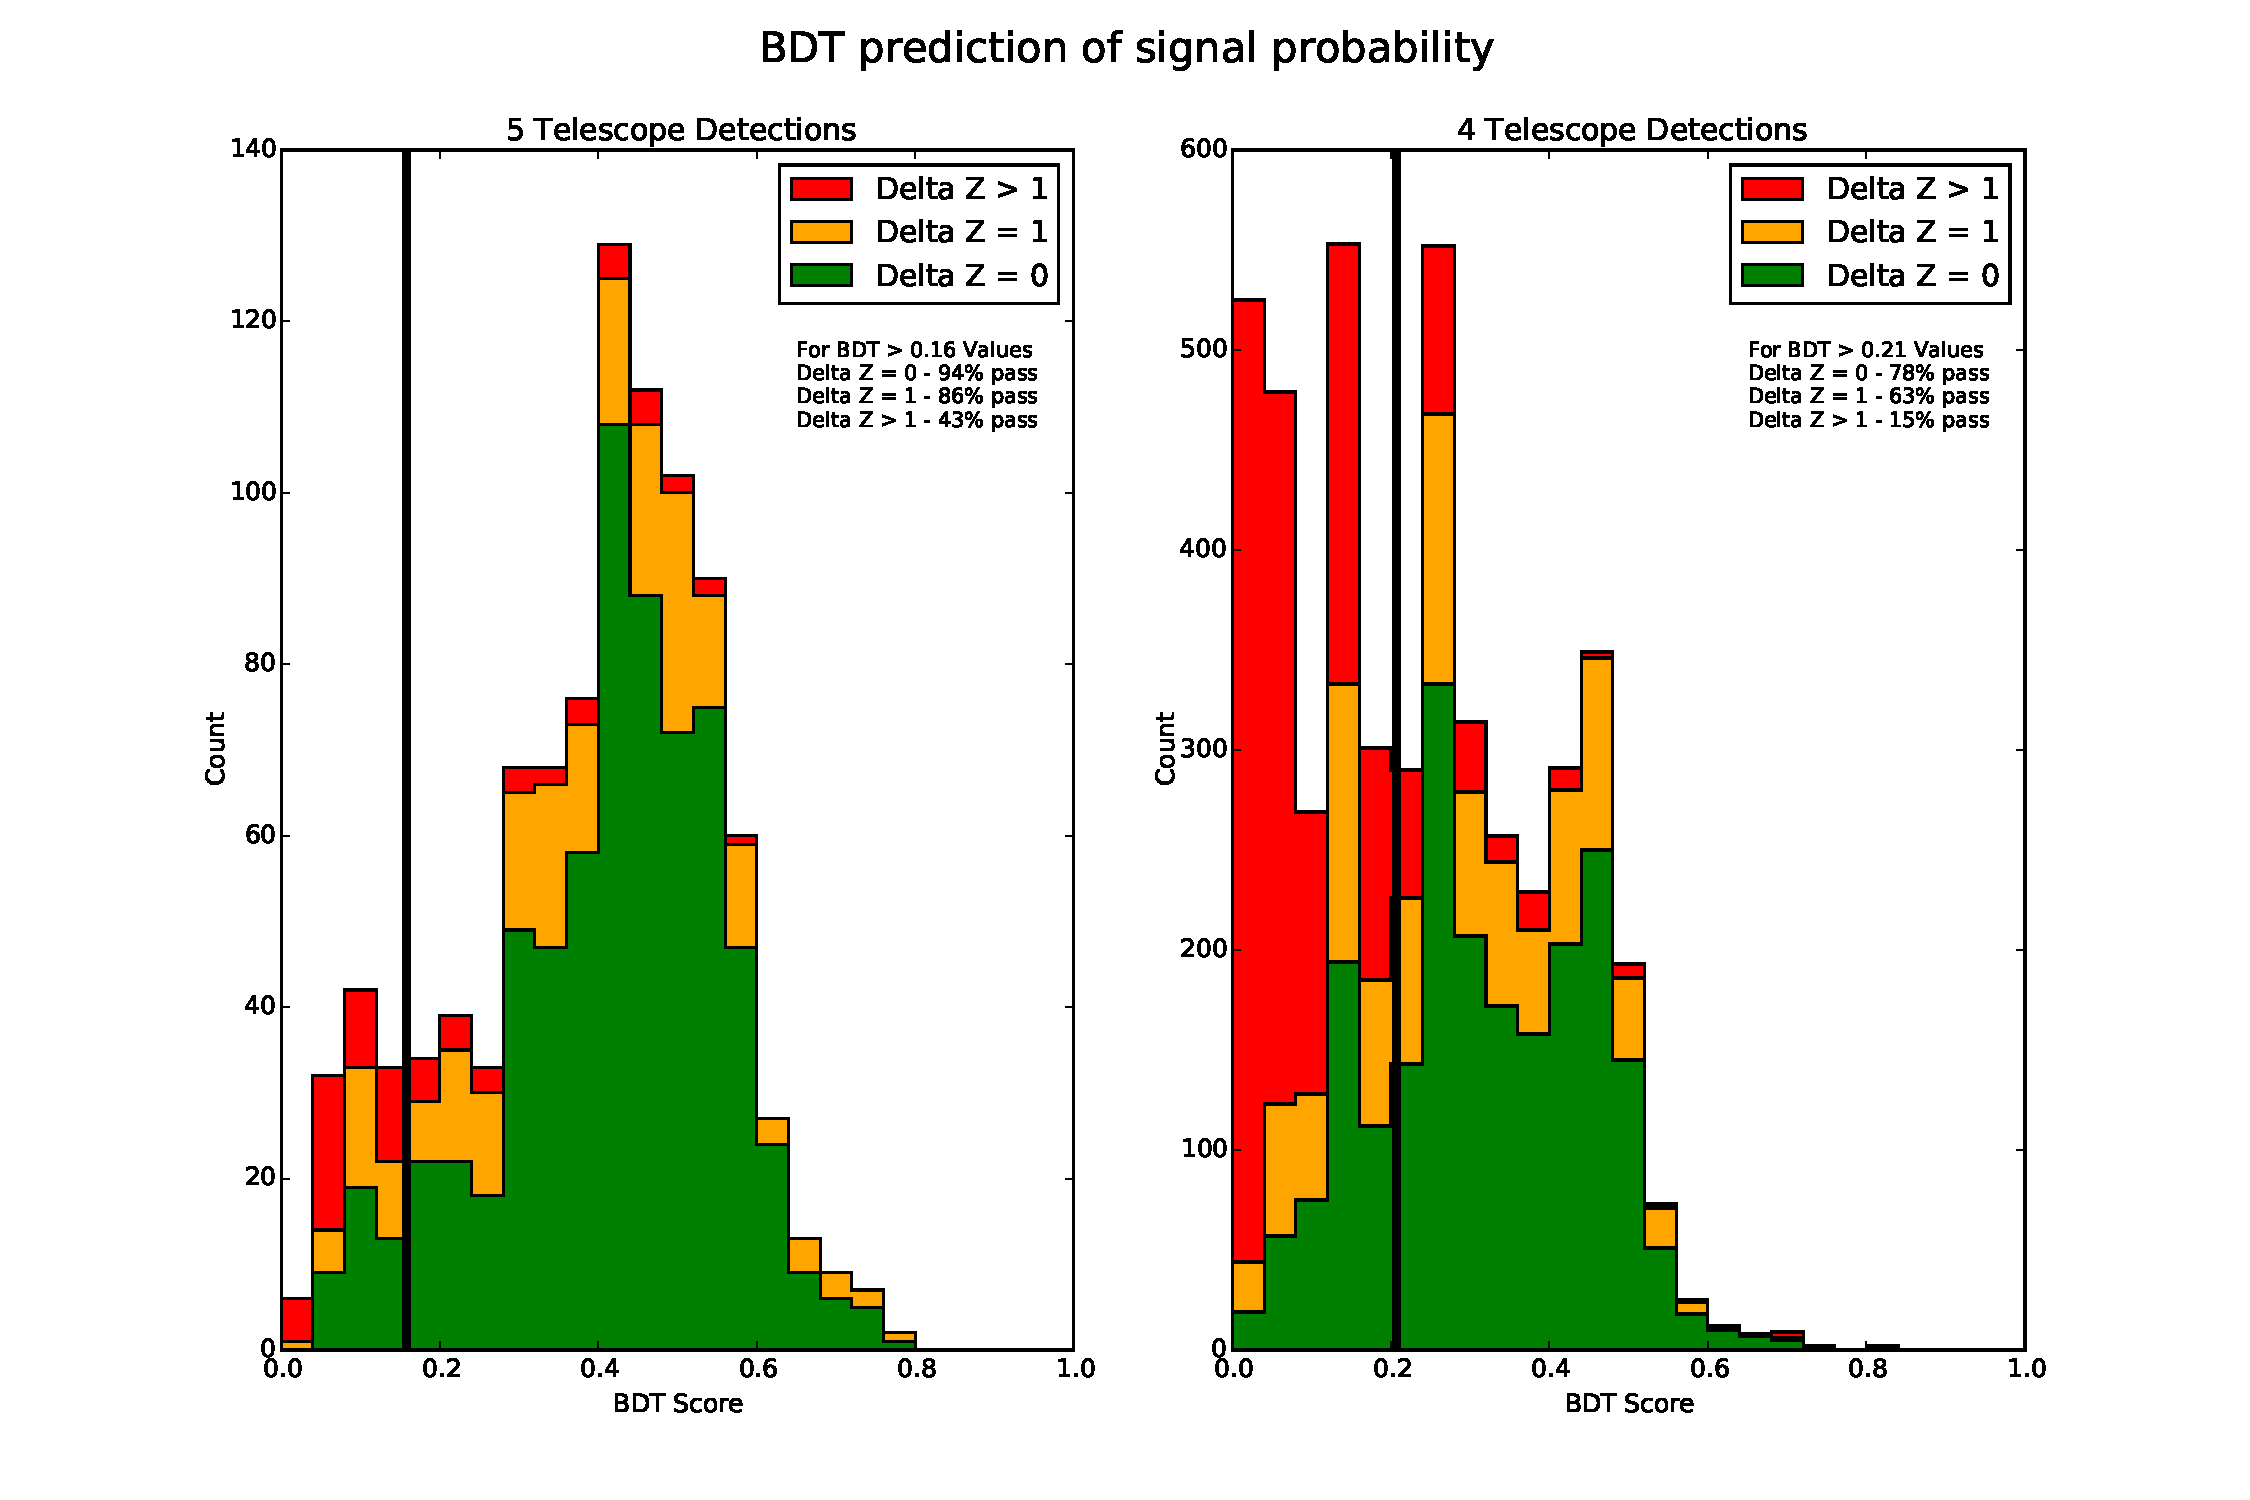
\includegraphics[width=\textwidth]{Likelihood}
\caption{The BDT score distribution is shown for the Monte Carlo test data. Events are colour-coded by how well the Charge number was reconstructed. We see that the majority of bad red events have a lower BDT score in the 4-tel graph. In each graph, the thick black line indicates the eventual cut made to the data.}
\label{fig:reconBDTdistribution}
\end{center}
\end{figure}

Having obtained a BDT score variables $P_{4tel}$ and $P_{5tel}$, we can then optimise cuts on this variable. The two BDTs will be optimised independently. Our aim is to reduce the value of $\sigma_{Z}$ to provide a narrower reconstructed peak. This should enable more effective spectroscopic analysis. At the same time, we wish to maintain as high a pass rate as possible, to reduce the expected random Poissonian Error in the dataset. We know that the Poissonian Error of a distribution scales with $\frac{1}{\sqrt{N}}$. Ultimately we expect to obtain a spectrum of overlapping Gaussians corresponding to each element, and fit for the relative height of each Gaussian. To balance the competing priorities of large N and small $\sigma_{Z}$ which will enable the Gaussian peaks to be resolved, we can define a new scaled variable $\mathbf{\tilde{\sigma_{Z}}} = \frac{\sigma_{Z}}{\sqrt{(f)}}$. Here, instead of N, we are scaling with the passing fraction of events $f = \frac{N_{passing}}{N_{total}}$. The quantity $\mathbf{\tilde{\sigma_{Z}}}$ is then found for a range of BDT cut values, and the minimum found. The values of $\sigma_{Z}$ and $\mathbf{\tilde{\sigma_{Z}}}$ are shown in Figure \ref{fig:Zcuts}. Ultimately, a cut of $P_{4tel} > 0.21$ and $P_{5tel} > 0.15$ was chosen, corresponding to $\sigma_{Z}=0.88$ and $\sigma_{Z}=1.04$ respectively. The respective passing fraction was 0.92 and 0.53. The improvement for 5 telescope events is minor, but for 4 telescope events there is a significant reduction in charge resolution.

\begin{figure}
\begin{center}
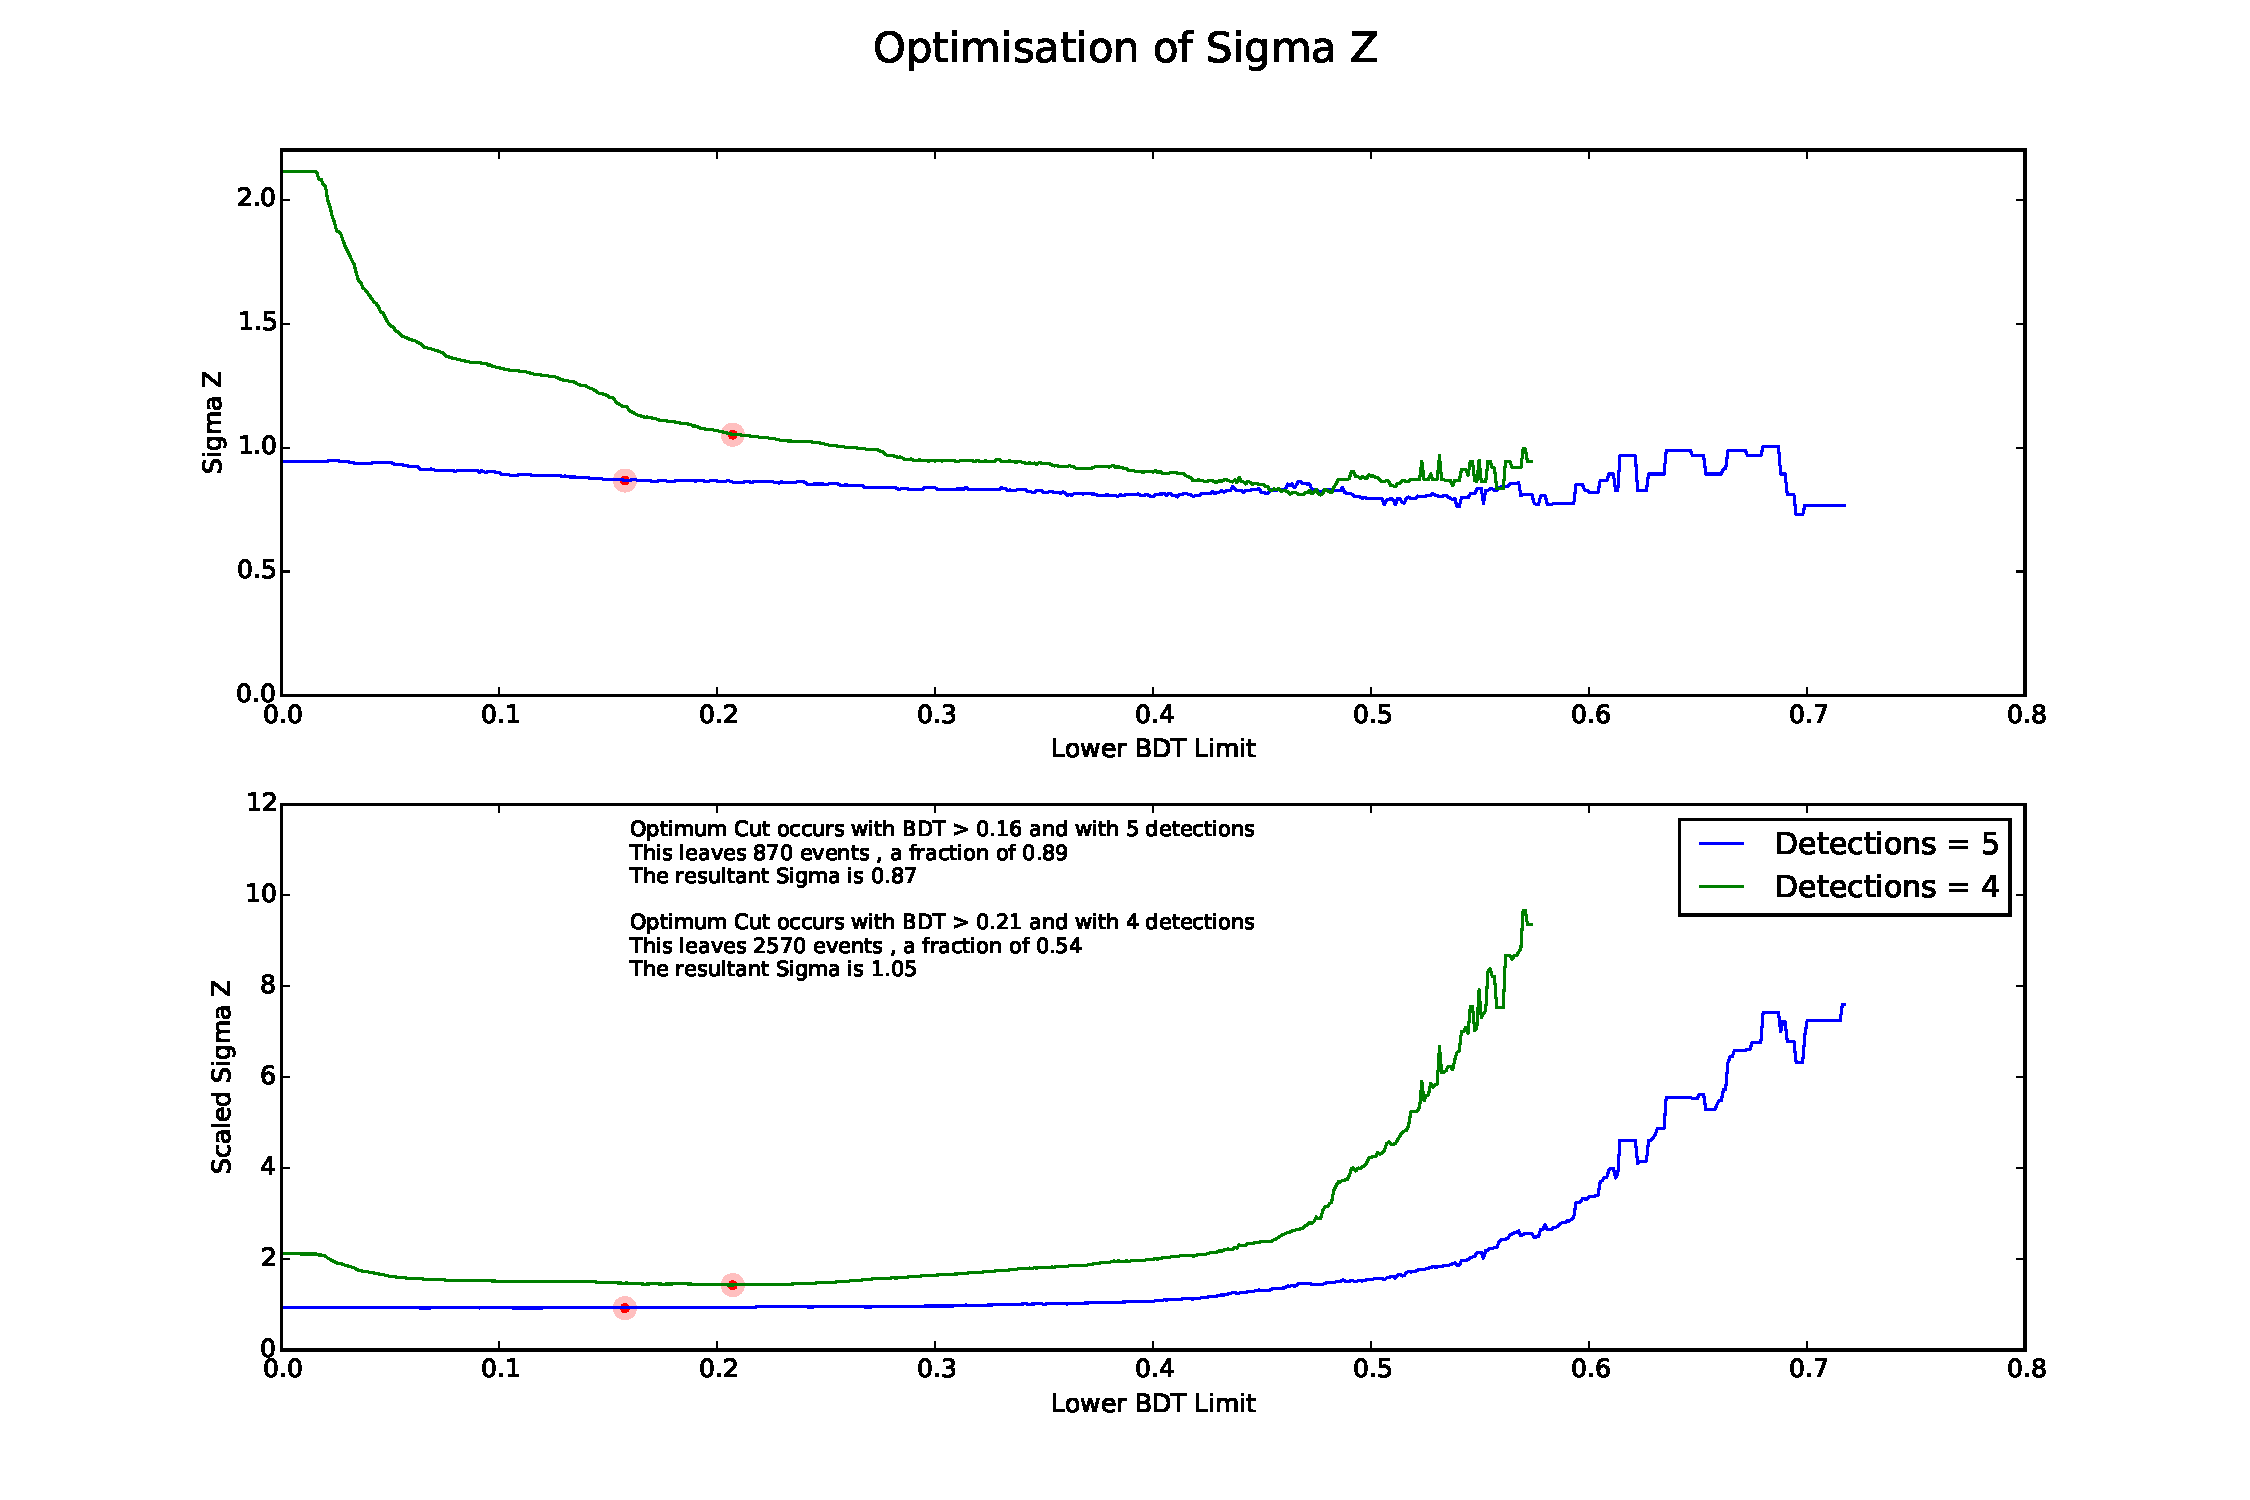
\includegraphics[width=\textwidth]{Zcuts}
\caption{Above, the raw values for $\sigma_{Z}$ are shown as a function of the BDT cuts for 4-tel and 5-tel events. Below, the scaled values of $\mathbf{\tilde{\sigma_{Z}}}$ are shown. For 4-tel events, there is a clear minimum for $P_{4tel} > 0.21$, while for 5-tel events, there is a broader minimum at $P_{5tel} > 0.15$.}
\label{fig:Zcuts}
\end{center}
\end{figure}

We can plot the distribution of reconstructed core positions, with the BDT score as a color scale. We see that a clear pattern emerges, with distinct differences between 4-tel and 5-tel events. For 4-tel events, the core positions are widely distributed in the simulated region. However, there are many cores clustered around each of the 5 telescopes. It is important to recall that the BDT is never explicitly told about the position or number of telescopes, though the distinct features at each telescope tell us that their existence has clearly been inferred by the BDT. This suggests that the BDT is functioning as we would hope, and has learned indirectly where the telescopes lie. 

This makes sense, as cores close to a telescope are likely to produce negligible DC light in that telescope. However, once the $P_{4tel}$ cut is applied, the majority of events lying outside the square of small telescopes are removed. Also, interestingly, most events lying near one of the smaller telescopes are removed, giving each telescope a noticeable halo containing few or no events. This suggests that, if an event lies close to one telescope, the distance to the opposite diagonal telescope is likely to be too large to produce a DC signal. Thus, we would instead expect a 3-tel event. We know that the first interaction height is reconstructed extremely poorly, and thus the exact $r_{max}$ values for these LPDs is uncertain. It is likely that, given this, the height is being misreconstructed to allow the LPD to extend far enough to trigger the most distant telescope.

However, there is a region of high $P_{4tel}$ points lying directly beyond the halo, in the inner region. Events in this location are likely to be too dim to trigger the nearest telescope, while still being close enough to trigger the remaining telescope. This region also encroaches partially on the four telescope halos that would otherwise be completely circular. We are left with a clear square region of high-score events lying within the telescope square. There is then a less distinct halo surrounding the central CT5 telescope. This halo represents events that would be distant enough from the center to trigger the CT5, but central enough to also trigger the outer 4 telescopes. within this halo, there is a dense region of reconstructed events lying very close to the CT5 telescope, where they are close enough to not trigger it but are still able to trigger the outer 4 telescopes.

The distribution of 5-tel events is much easier to explain. As each telescope must be triggered there is a clear halo surrounding each telescope. Certain events are reconstructed with a higher radius from the center, and these are mostly removed by the $P_{5tel}$ cuts. We are left with a ring surrounding CT5 of high scoring events. The relatively loose cut is extremely effective at reducing almost outlying events that are far from the centre, while leaving almost all other events. Future reconstruction techniques could aim to make use of this information by restricting the core position to these regions of expected high-multiplicity. However, this was not done as part of this analysis. 

\begin{figure}
\begin{center}
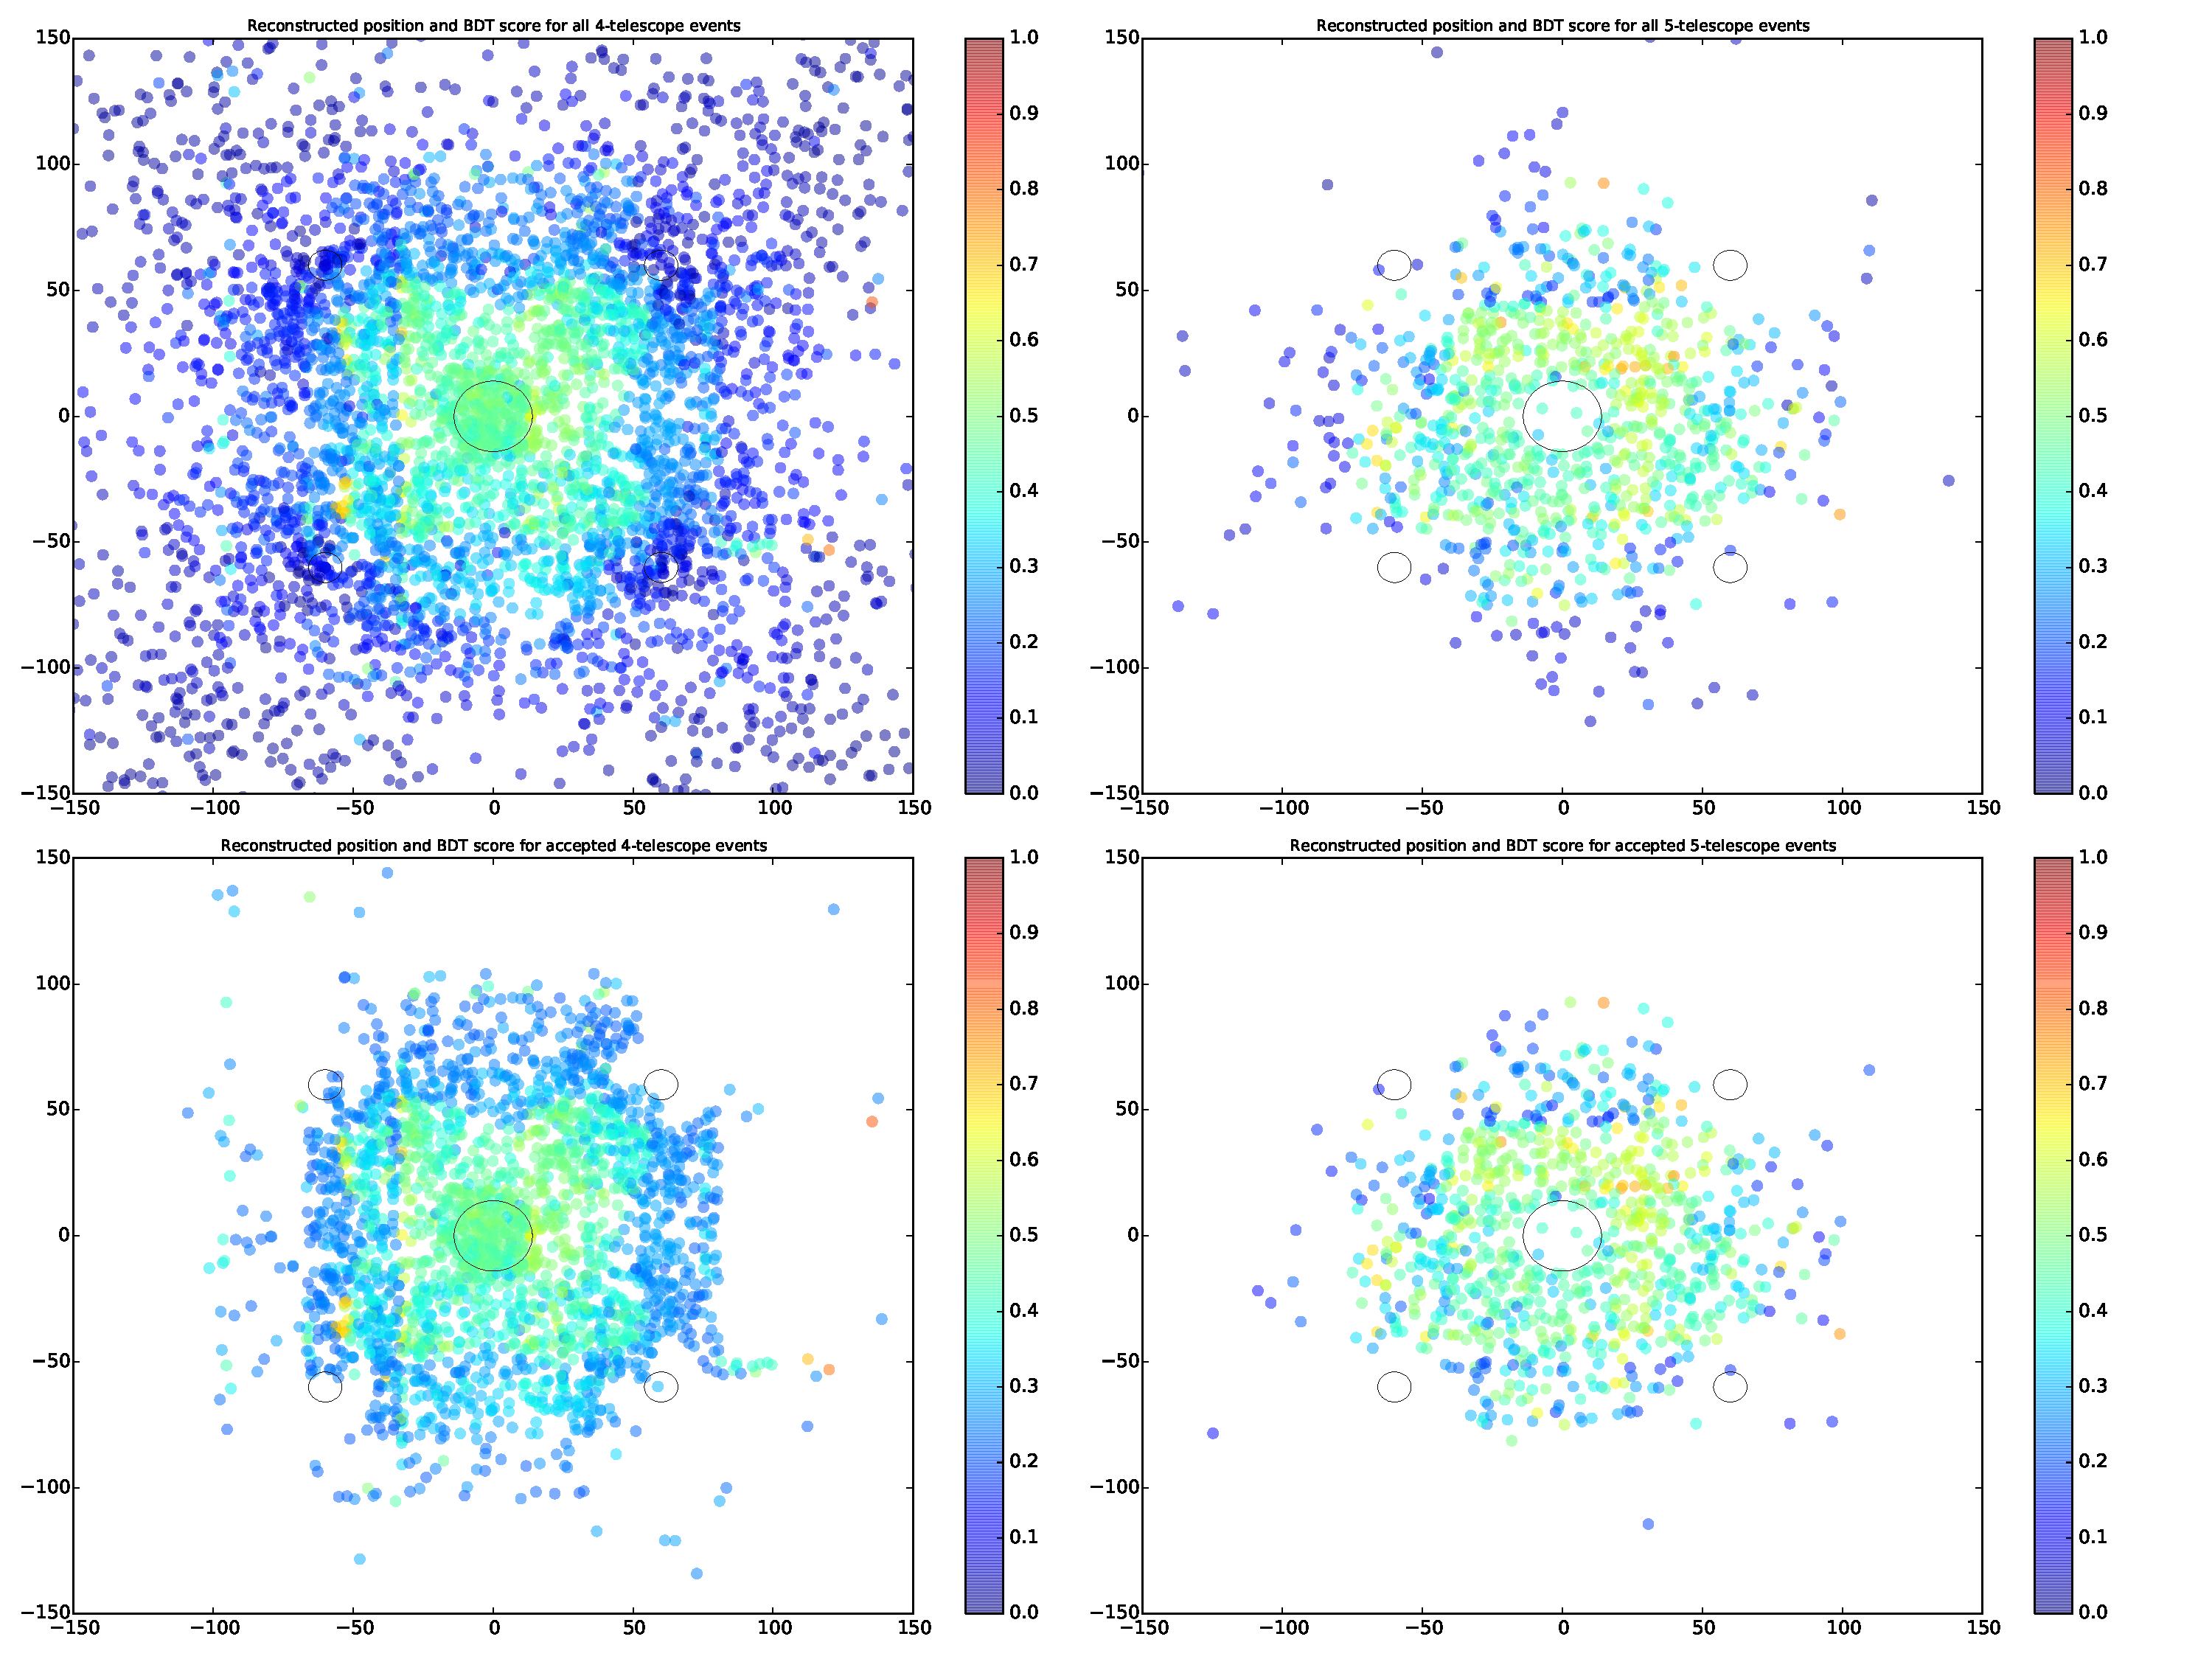
\includegraphics[width=\textwidth]{bdtmap}
\caption{A geometric representation the reconstructed events is shown. Each coordinate corresponding to a reconstructed position in metres. The 5 HESS telescopes are represented by black rings. Above we see all events, while below we see only events passing their respective BDT cuts. In the left column we see the 4-telescope events, while in the right column, we see 5-telescope events.}
\label{fig:bdtmap}
\end{center}
\end{figure}

We can assess the impact of the $P_{4tel}$ and $P_{5tel}$ cuts on the distribution of reconstructed Energy. We would expect that the true energy distribution would begin at around 10-15 TeV, when Cherenkov Emission becomes possible. The number of events would increase with energy up to a maximum around 25 TeV when Emission becomes saturated, and would then decline in accordance with the $E^{-2.7}$ flux rate. The reconstructed Energy distribution does, as expect, follow this pattern. This suggests that our method for Energy reconstruction is reasonable, and this is further confirmation of the reasonably precise energy resolution shown in Figure \ref{fig:rawepn}. The Energy distribution is shown in Figure \ref{fig:energy}, alongside the post-cuts distribution. The full simulated distribution of $\phi(E) \propto E^{-2.7}$ is indicated alongside the reconstructed distributions. There is already a noticeable similarity between the Simulated and Reconstructed Energy distributions, albeit with a broadening due to the Energy resolution of roughly 10\%. 

As might be expected, the loose $P_{5tel}$ cuts produce little noticeable difference to the distribution. However, there is a clear curtailing of the lower Energy events after the $P_{4tel}$ cut has been applied. This is as might be expected, because events that are not saturated in Energy are unlikely to be reconstructed well. Ultimately, the post cut distributions of 4-tel events appears similar to the 5-tel distribution, albeit with a greater overall frequency. Both lie closer to the simulated distribution once cuts have been applied. In contrast, the pre-cuts 4-tel events had a noticeable broader distribution extending further into the very low and very high energy regimes even when compared to the 5-tel rather than simulated distribution. The results broadly vindicate our decision to apply an Energy Cut on reconstructed events that was implemented to remove protons. Were the lower Energy Iron events to have been included in our simulations, we would have needed to remove them through the BDT method because they are unlikely to be reconstructed well. Having applied the BDT cuts, we see that the 5-tel distribution broadly follows the simulated distribution with a relative height of 0.6\%, while the 4-tel events follow the simulated distribution with a relative height of 1.8\%. 

\begin{figure}
\begin{center}
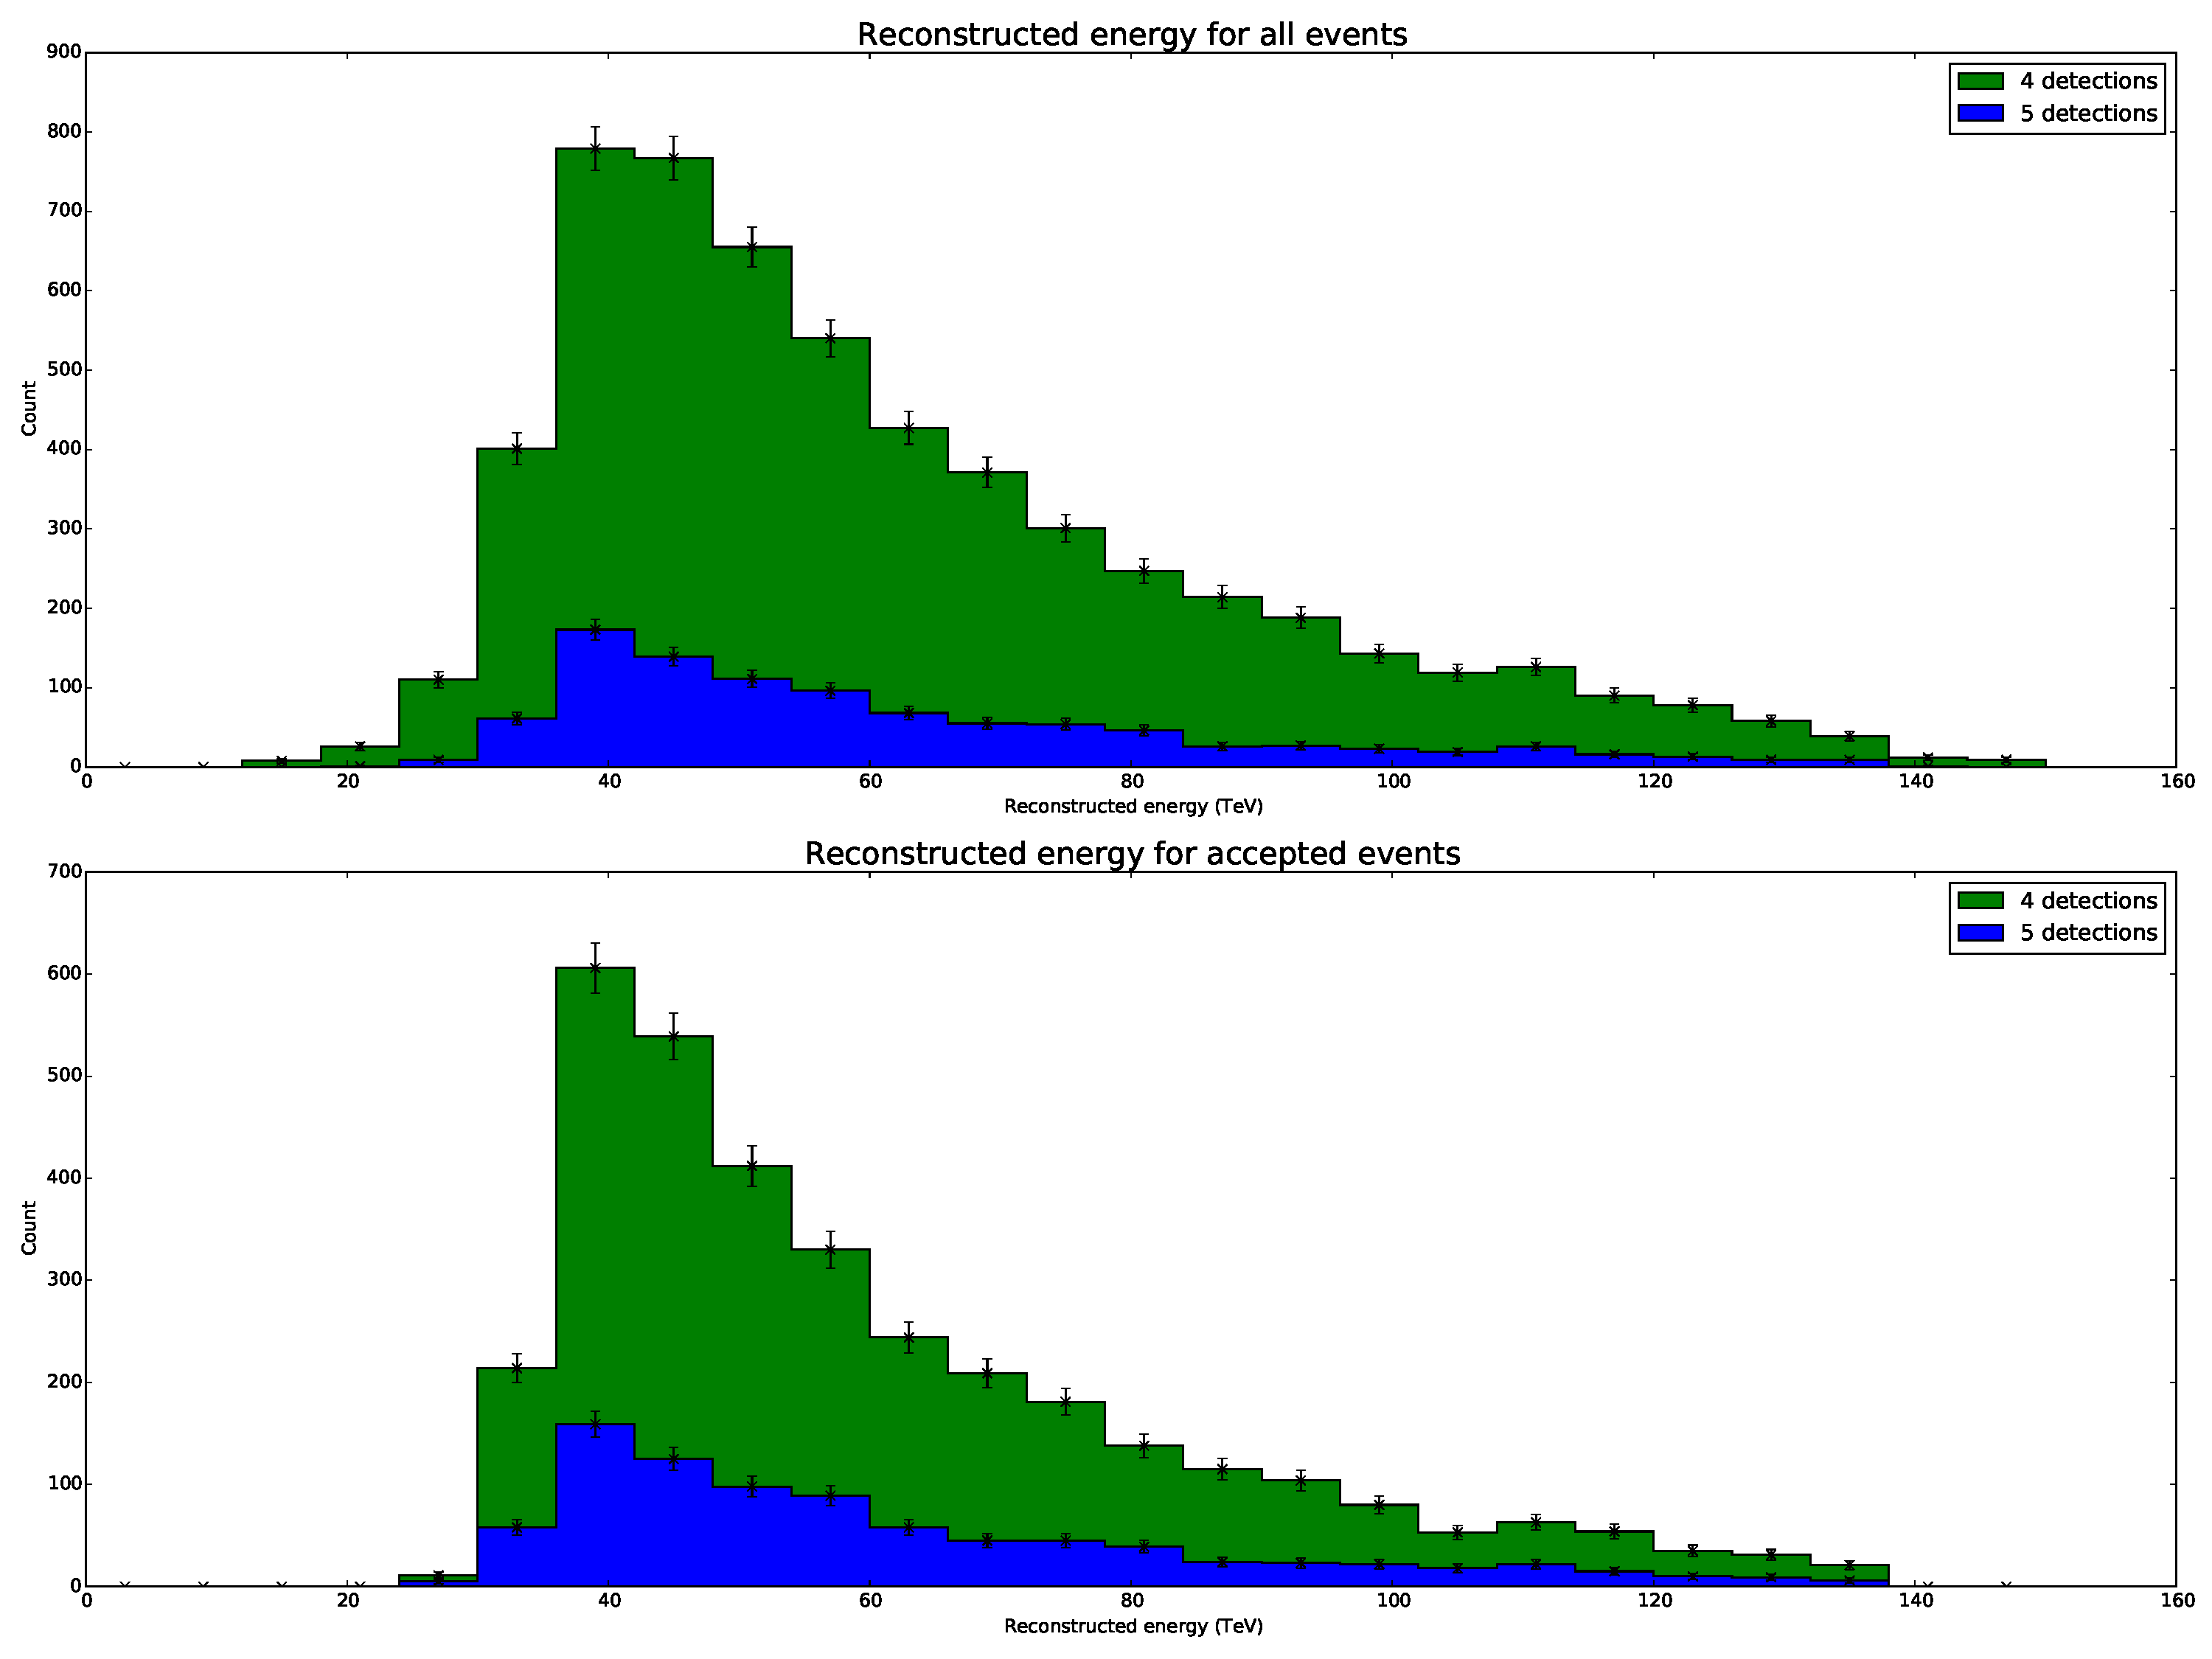
\includegraphics[width=\textwidth]{energymap}
\caption{The reconstructed Energy distribution is shown. Above, all events are included. Below, only those events passing the $P_{4tel}$ and $P_{5tel}$ cuts are included}
\label{fig:energy}
\end{center}
\end{figure} 

\subsection{Final Variable resolution}
After application of the BDT cut to the Monte Carlo datasets, the distributions in Energy, Core Position and
Charge are repeated. Unsurprisingly, the loose cuts for $P_{5tel}$ mean that 5-tel performance is only slightly improved, while the 4-tel performance is more significantly improved. For 5-tel events, the core position reduces from $\sigma_{core} = 9.2m$ to $\sigma_{core} = 8.7m$, while for 4-tel events, the improvement is a substantial reduction from $\sigma_{core} = 17.0m$ to $\sigma_{core} = 10.0m$. Ultimately our resultant core resolutions are broadly similar for both multiplicities, and represent a significant improvement over previous Hillas-reconstructed core positions. Considered as a target region, we see that we have a roughly fourfold reduction in bounding area likely to contain the core. 

With regards to energy, the removal of many low-energy events by the 4-tel BDT leads to a clear improvement in resolution. This is evident in Figure \ref{fig:epn}. The 5-tel resolution improves slight from $\frac{\sigma_{E}}{E} = 0.06$ to $\frac{\sigma_{E}}{E} = 0.05$ and the 4-tel resolution improves more noticeably from $\frac{\sigma_{E}}{E} = 0.12$ to $\frac{\sigma_{E}}{E} = 0.06$. We again see that the harsher $P_{4tel}$ cuts leads to a convergence of 4-tel and 5-tel resolution. The height resolution remains poor, but continues to not hinder the charge reconstruction.

This trend continues for the charge resolution, where we see a sharp improvement for 4-tel events. Whereas in Figure \ref{fig:rawZ} the distribution is clearly partially truncated by the imposed range of $16 < Z < 36$, we see no such problem once $P_{4tel}$ cuts have been applied. Ultimately the 5-tel resolution improves from $\sigma_{Z}=0.95$ to $\sigma_{Z}=0.88$, while the 4-tel resolution improves from $\sigma_{Z}=2.11$ to $\sigma_{Z}=1.05$. In doing this, we have achieved our stated aim of obtaining a charge reconstruction method capable of producing large datasets with a charge resolution of roughly  $\sigma_{Z} \approx 1$. The LPD method is this shown to be sufficiently good to enable spectroscopic analysis of Heavy Cosmic Rays. 

\begin{figure}
\begin{center}
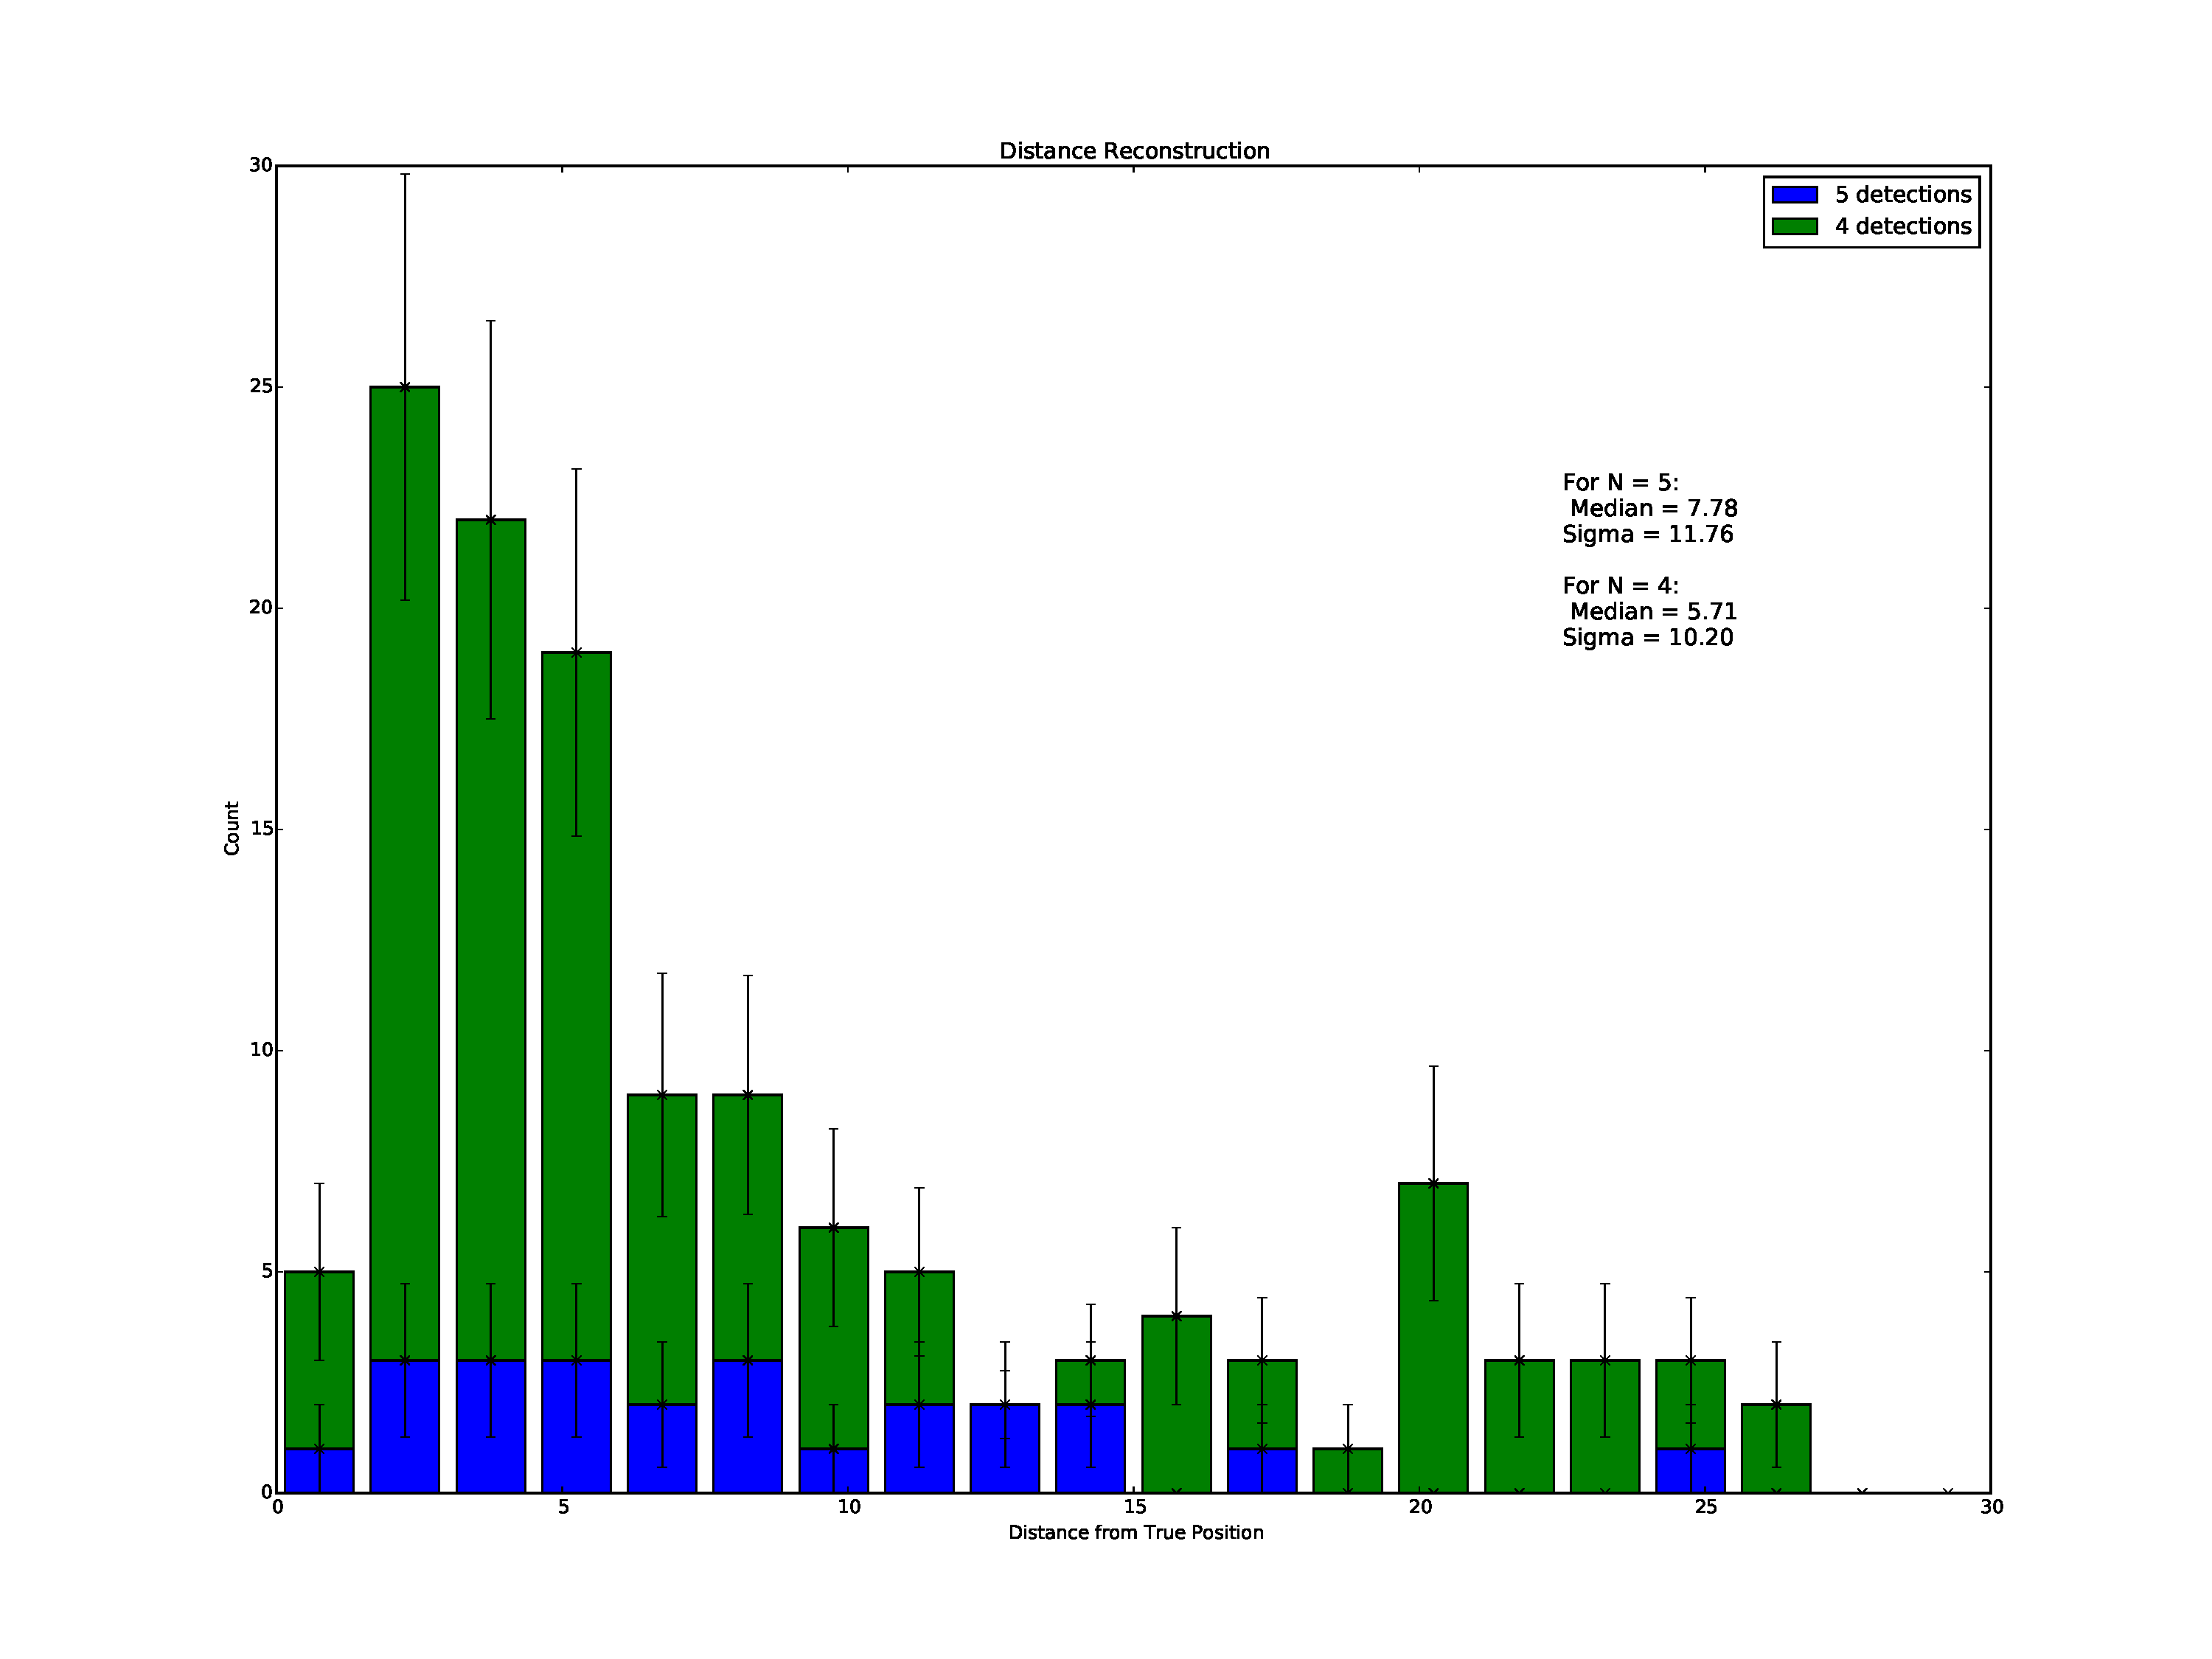
\includegraphics[width=\textwidth]{position}
\caption{The distance from true core position to the reconstructed core position is shown above. For 4-tel events, the standard deviation from true position is 10.0m, while for 5-tel events, it is 8.7m.There is a clear improvement over the distribution in Figure \ref{fig:rawposition}.}
\label{fig:position}
\end{center}
\end{figure}

\begin{figure}
\begin{center}
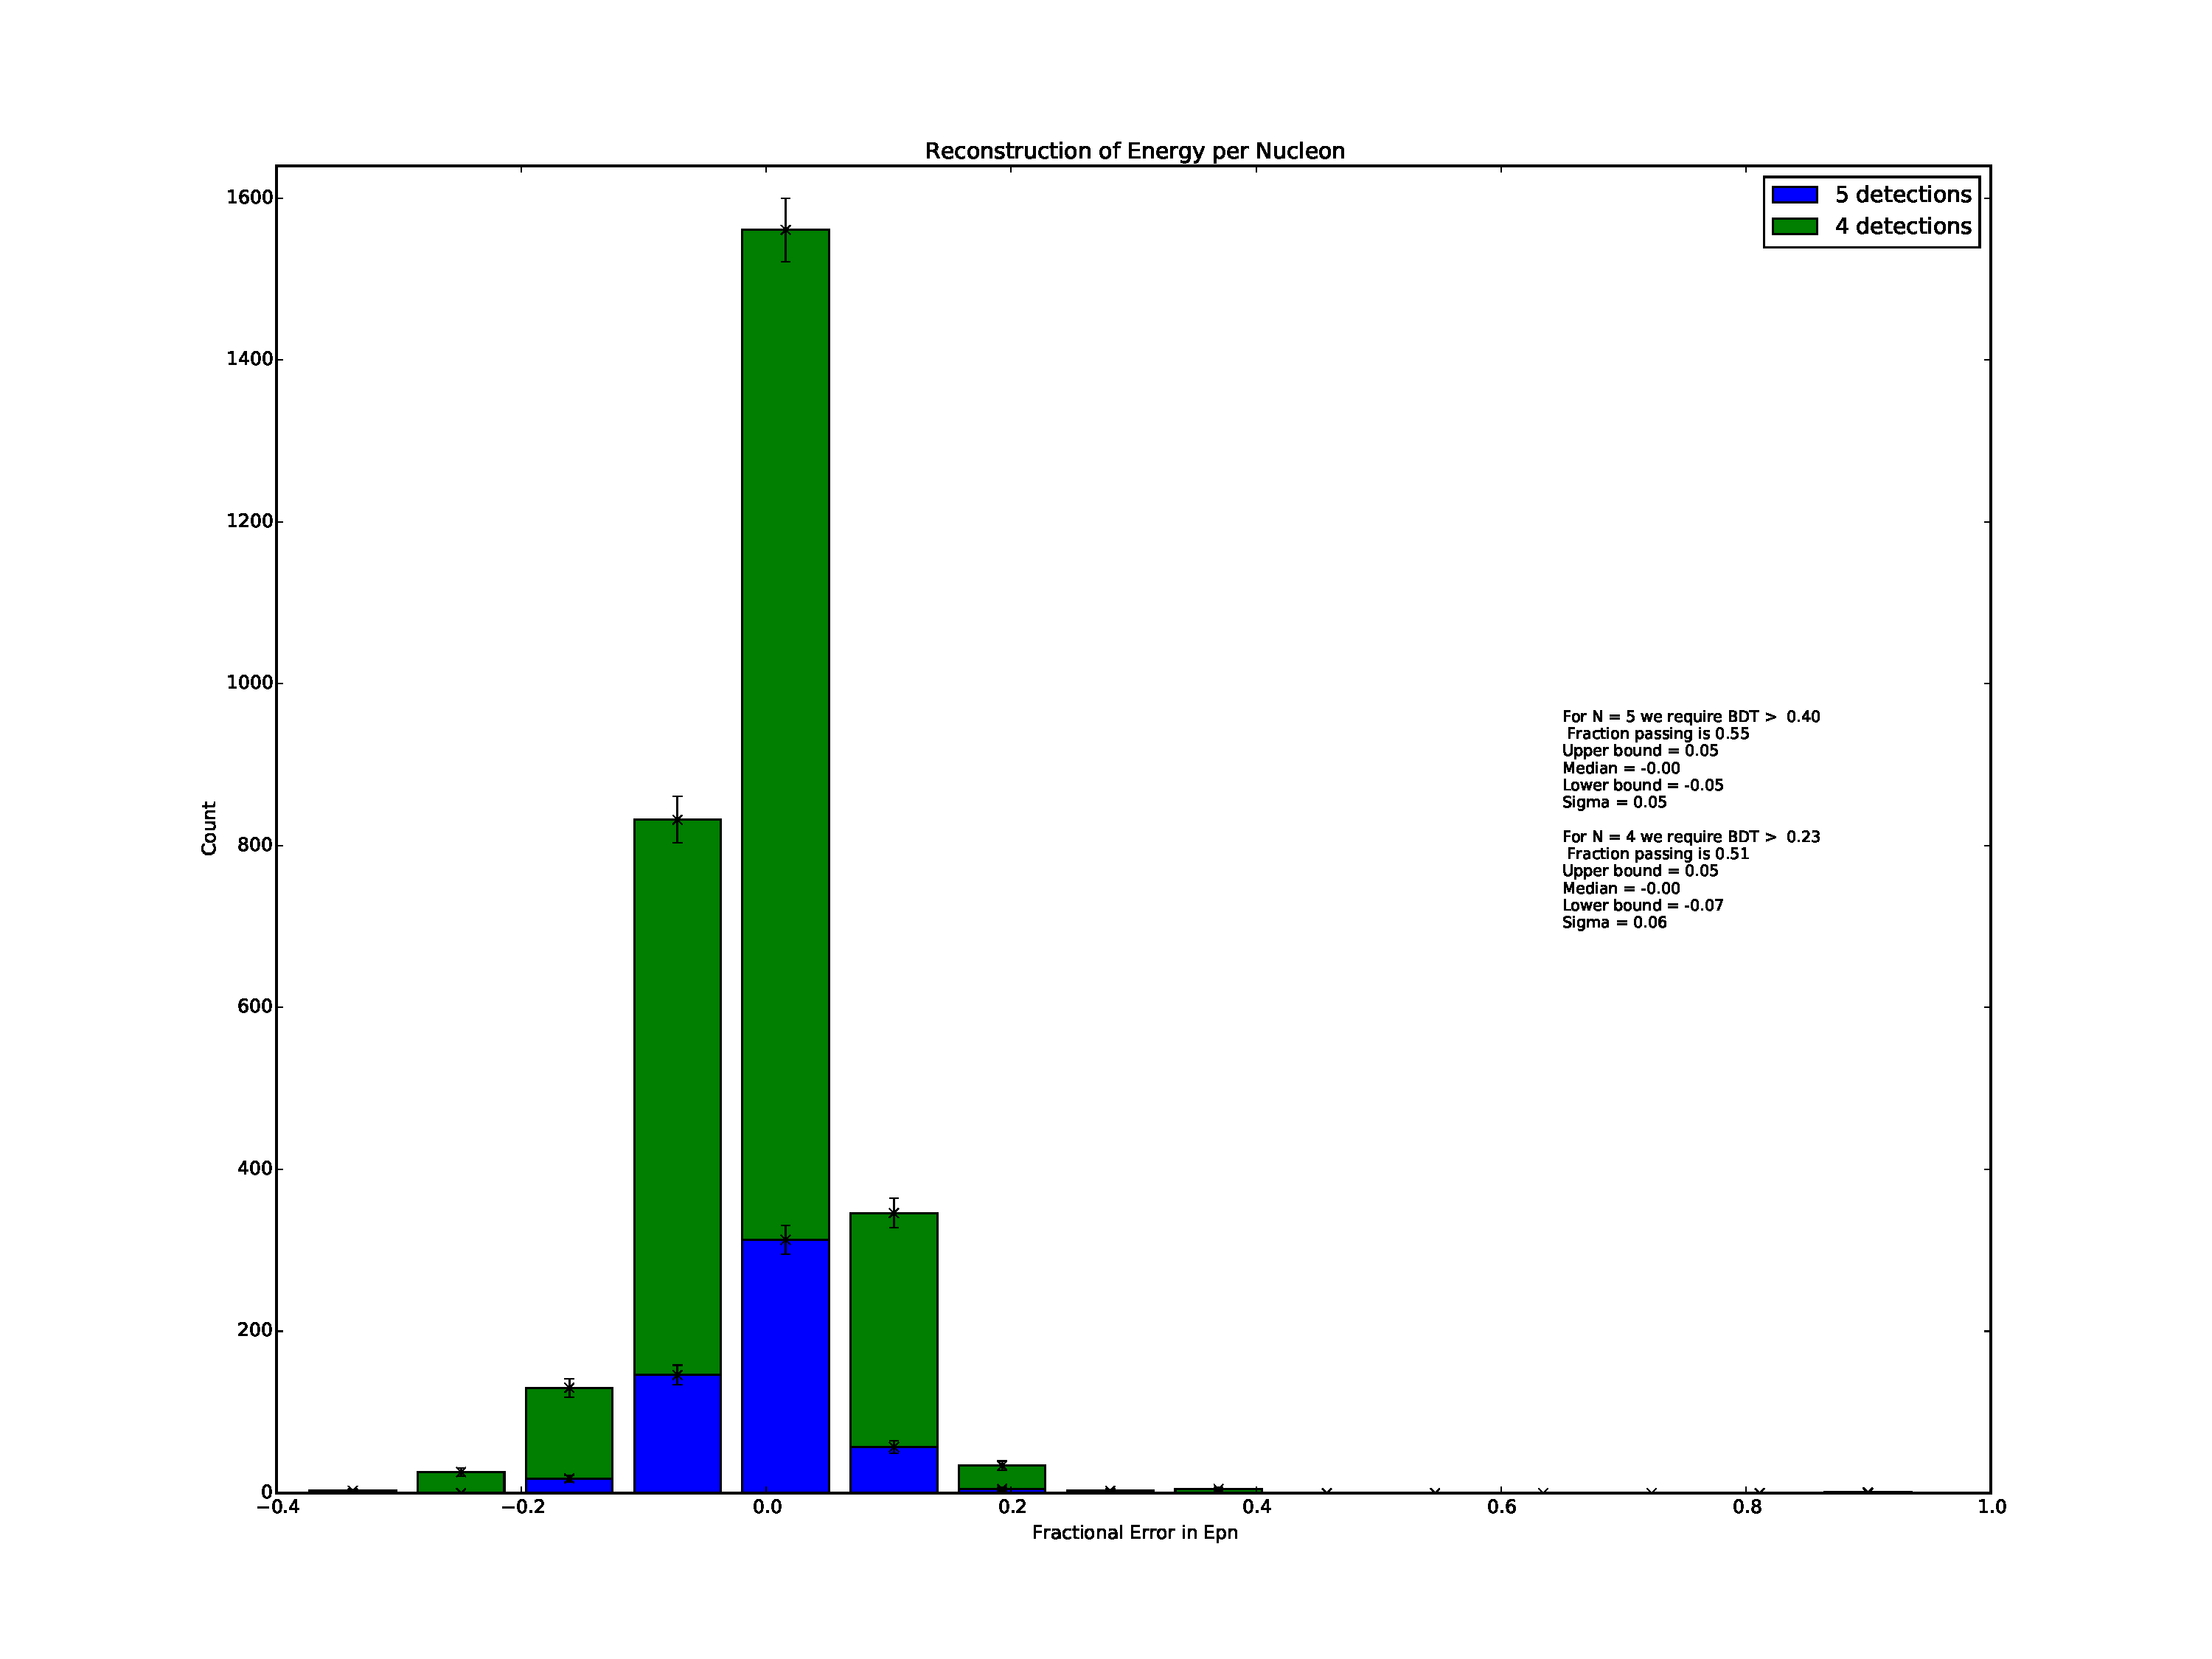
\includegraphics[width=\textwidth]{epn}
\caption{The fraction deviation from true energy is shown above. For events with five-telescope multiplicity, the fractional error is 0.05 but for four-telescope multiplicity, it is 0.06. The expected poissonian error bars are also shown. There is a clear improvement over the distribution in Figure \ref{fig:rawepn}.}
\label{fig:epn}
\end{center}
\end{figure}  

\begin{figure}
\begin{center}
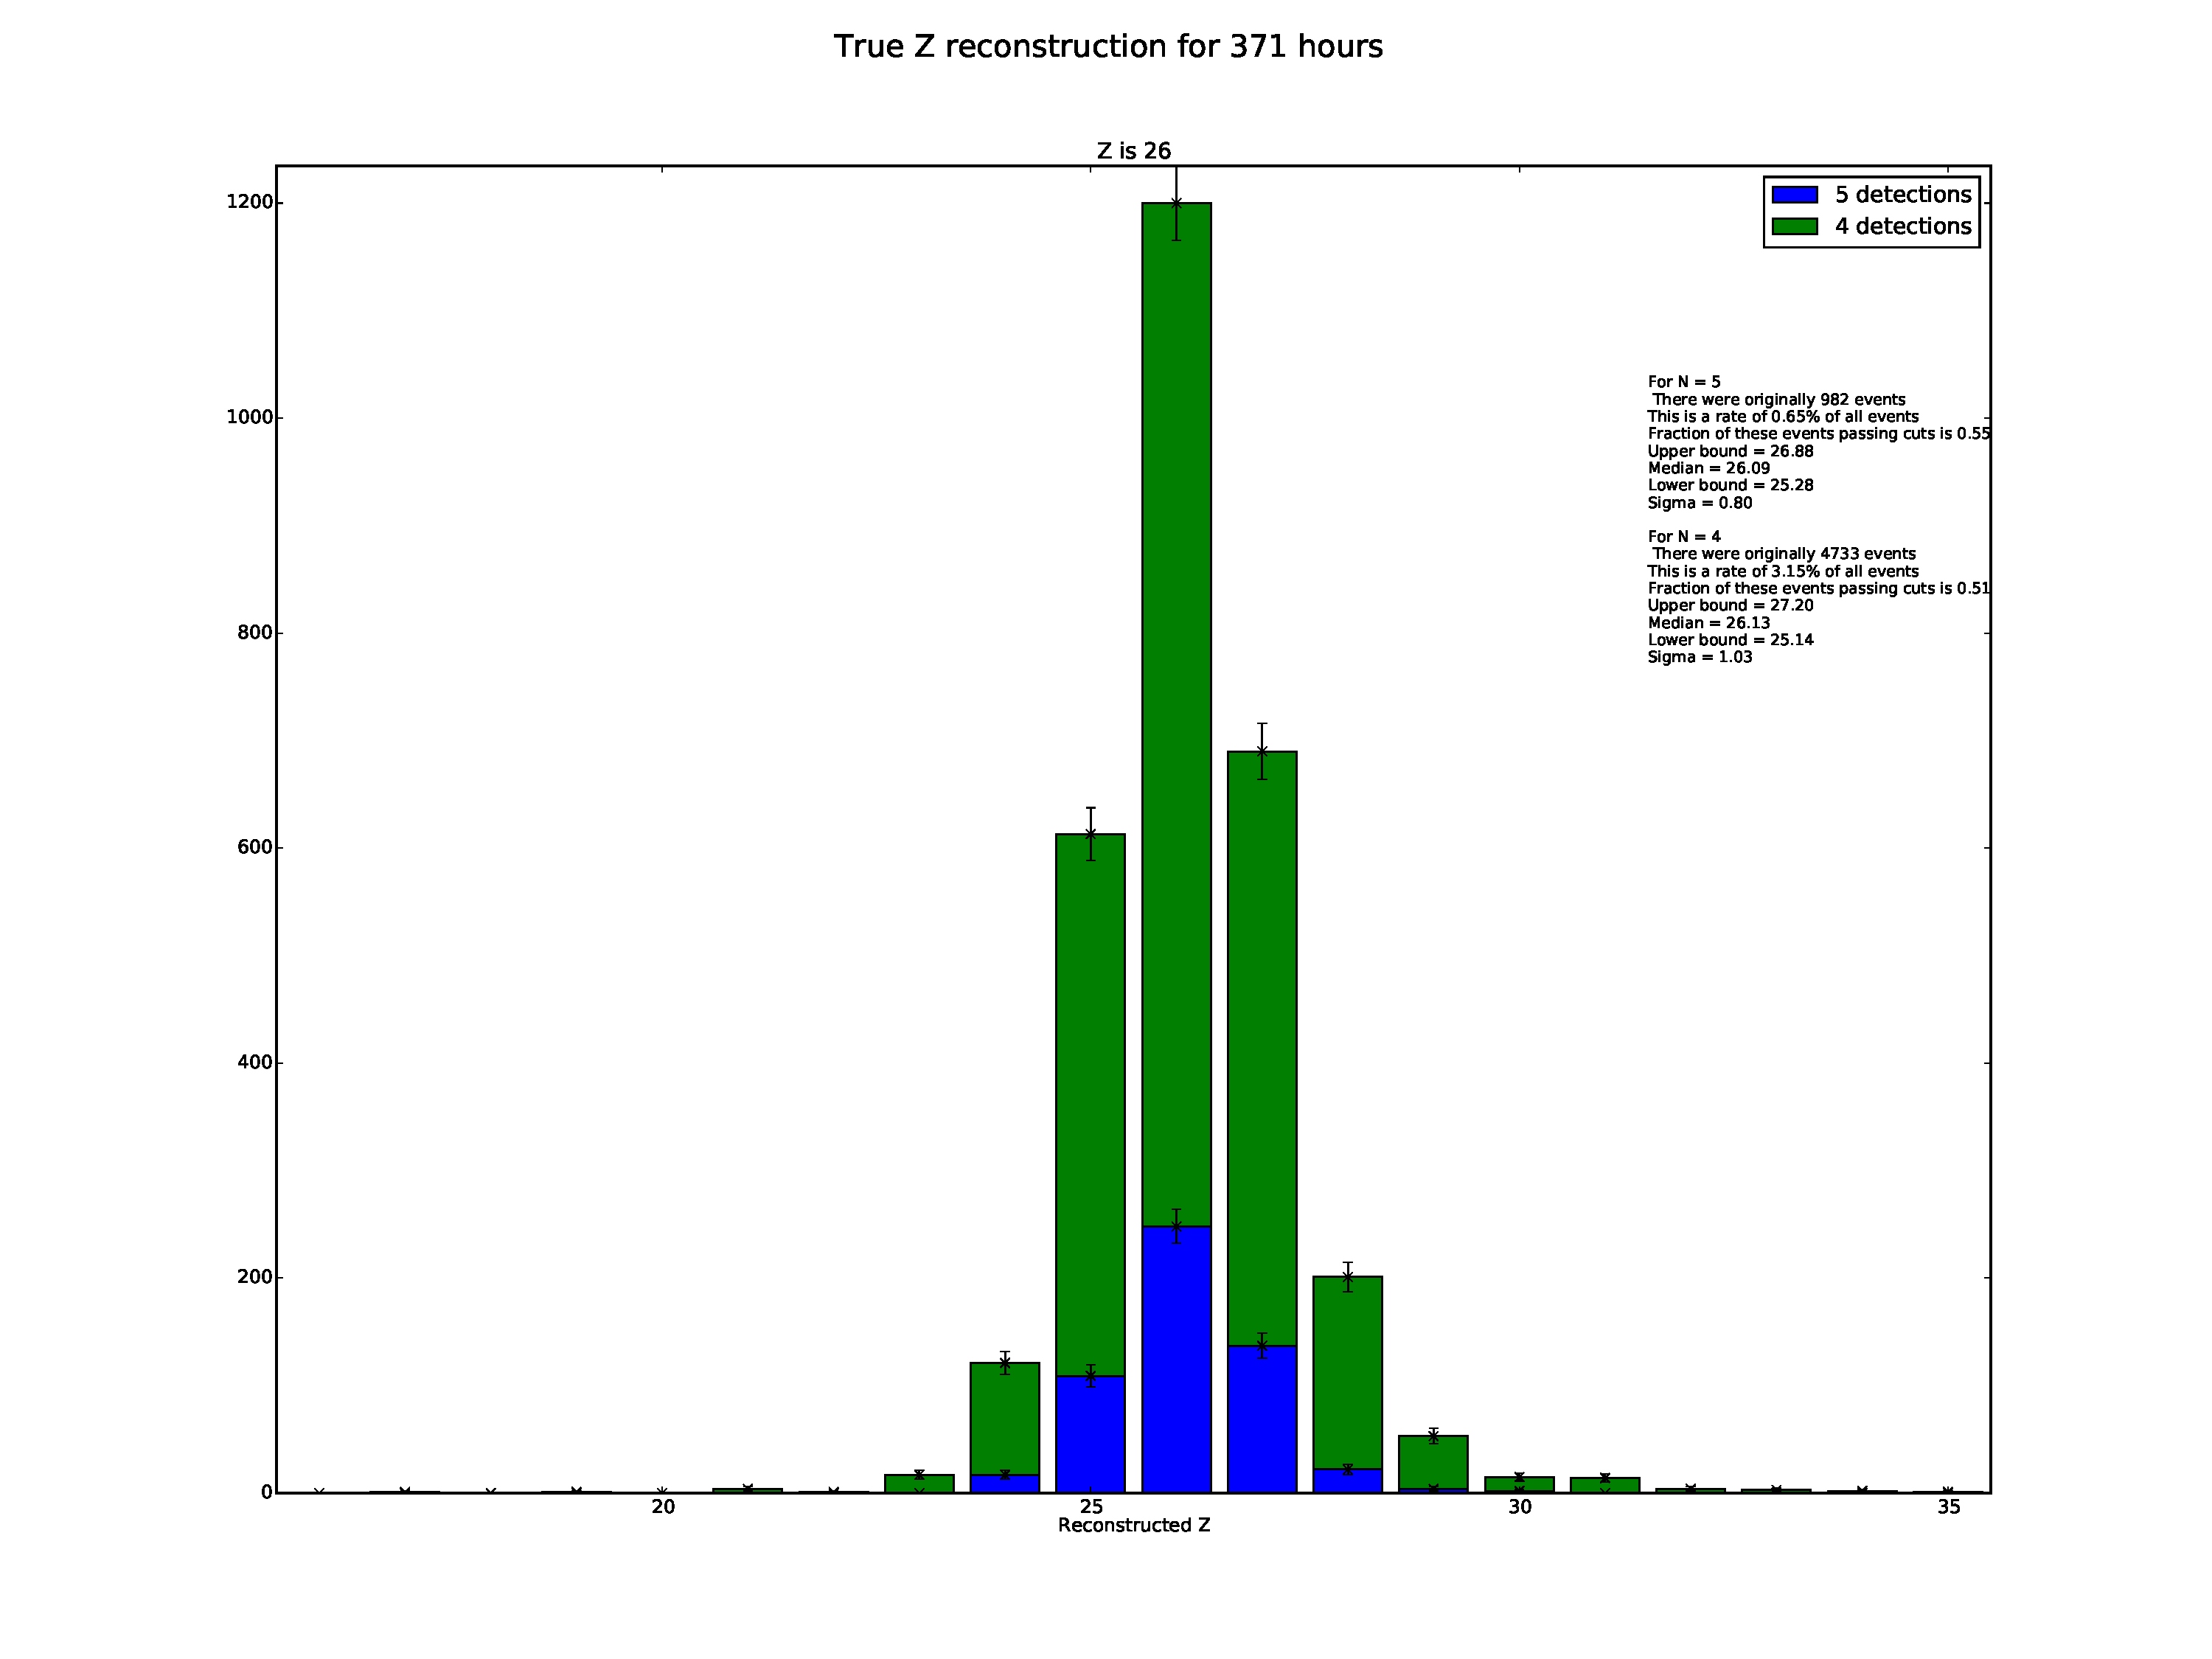
\includegraphics[width=\textwidth]{Z}
\caption{The reconstructed charge for the cut dataset is shown, with a clear peak around the true value of Z=26. There is a noticeable improvement over Figure \ref{fig:rawZ}, with a new resolution of 1.1 and 0.9 for 4-tel and 5-tel events respectively.}
\label{fig:Z}
\end{center}
\end{figure}


\section{Further Improvements}
There are many potential avenues that would improve or expand upon the work conducted as part of this analysis. The development of a new method of DC pixel identification is likely to prove particularly useful, as it performs more accurately and vastly more efficiently that existing methods of DC pixels.  

\subsection{Hillas Reconstruction}
The LPD reconstruction method was developed to replace the current method of Hillas Reconstruction, owing to the latter's poor position resolution. Rather counter-intuitively, despite the demonstrated superiority of the LPD method, the result of this analysis may well be to strengthen the use of Hillas Analysis. The exact process for Hillas Reconstruction relies on deriving the Major and Minor axis of a shower image, and calculating pairwise intersection points of the major axes between telescopes to find the shower direction. Due to the blurriness of the shower images, there is significant uncertainty in placing of the major axis. However, we know that the major axis will pass through both the shower centre of gravity and the DC light. The shower centre of gravity is much easier to determine despite image blurring, and thus has a much lower uncertainty. Previously, difficulty in identifying DC pixels meant that this centre of gravity was not particularly useful. However, through use of the BDT-identified DC pixels, it should be possible to much more reliable place the major axis in a shower image. We can thus expect that, with the BDT, Hillas reconstruction may have a significantly improved core position resolution. Further analysis in this area will be conducted by other members of our research group. In the reasonable assumption that this does produce much better position resolution, we will have third independent method to determine the core position as well as the two LPDs. We could then conduct a likelihood minimisation encompassing this new information alongside the existing LPDs. We would expect our final core position resolution, and thus charge resolution, to improve even further as a result of these extra measurements.

\subsection{Actual Data}
The obvious next step to take as part of this analysis would be to apply the reconstruction method to real HESS data. We would hope to obtain a distribution similar to that in Figure \ref{fig:Z}, to which we could fit Gaussians centered on each integer value of Charge. In this way, we could calculate the relative abundance of the different Heavy Cosmic rays. Comparing the width of these Gaussians would confirm whether or not our reconstruction method was optimistic in our various assumptions for error. Additionally, on the basis of the calculated expectation rate for Iron Events we could compare to see if this agrees
with the data. An excessive experimental count rate would likely indicate that additional sources of background, such as protons, are passing the various cuts. To compensate for this, additional cuts would need to be designed and applied, which would likely lead to reductions in expected Iron acceptance rate.

In the event that the experimental method proves successful, it should be possible to use the exact position of the iron peak as a method of calibration for atmospheric absorption. An underestimate of the CORSIKA absorption used in training would lead to an iron peak that was shifted to a charge number lower than 26, due to a lower than unexpected photon count. Similarly, the reverse would apply if the modelled atmospheric absorption was an overestimate. As there is much associated uncertainty in the atmospheric properties, this would be a useful measurement to perform.

\subsection{High Speed Telescopes}
By definition, a Cherenkov-Emitting Cosmic ray will be travelling faster than the light that it emits. The EAS shower will thus arrive on the ground shortly before the DC light. There are currently several ultra-high-speed Cherenkov telescopes capable of resolving the received light into narrow time bands. It should thus be possible for the telescope to directly measure the DC light in one image, and the EAS shower in another image. We can imagine the possible impact that such a telescope array would have on the reconstruction process. Directly measuring this light will provide a direct measurement of $True_{DC}$ for use in shower reconstruction. Although we saw that the value of $True_{DC}$ has a relatively large associated error, it could be used in various ways. Firstly, it could be used as an additional measurement to give a third LPD to be minimised. These extra $True_{DC}$ measurements could be included in any likelihood minimisation. Secondly, we could use the observation or non-observation of DC light to more reliably constrain the core position of DC light. At present, our reconstruction method can have a BDT-identified DC pixel even though there may not actually be DC light in the image. Thirdly, the $True_{DC}$ variable could be passed to the regressor that was trained on the full shower images. It is possible that this information may correlate well to other variables, and enable better regressor LPD reconstruction.

\subsection{Optimised Telescope Array}
The reconstruction process that was developed is generally applicable to all telescope arrays that image Cherenkov Light. This includes the Cherenkov Telescope Array (CTA), a planned array that is likely to have many more telescopes than HESS. As we have seen, the reconstruction process only works well for high-multiplicity events, but these represent only a small fraction of all HESS events. We can imagine how the expected Iron event rate might increase, were an alternate telescope array used. As the design for CTA has not been agreed, we can imagine what an optimum arrangement for CTA might be, for the purpose measure DC light using the method described here. To this end, we can consider a 3x3 array of Cherenkov Telescopes, which we want to use for identifying Cosmic Ray Elements accurately. We can vary the grid spacing, and determine the effect on expected count rate. In Figure \ref{fig:optmiselayout} we see the expected distribution of event multiplicities for varying grid width. While the overall detected event rate increases as grid width increases, we find that that the \textquoteleft High Multiplicity Count Rate' of events observed by 4 or more telescopes decreases with increasing grid separation. Competing with this effect is the reliance of LPD reconstruction on sampling the entire lateral distribution. Thus the reconstruction quality for a given multiplicity will likely decrease as Grid Width decreases. Nonetheless, it appears that the optimum grid spacing will likely lie in the 20-50m region to provide a reasonable count rate. This is likely to fully sample an LPD of typical radius $r_{max} \approx 100$, while clearly maintaining a reasonably high count rate. Further study of $\sigma_{Z}$ in this region is required to determine the optimum layout for event reconstruction, which is not necessarily a grid. Additional study in this area would be required to confidently predict what an optimum Cherenkov Array for Heavy Charge measurement might look like.

\begin{figure}
\begin{center}
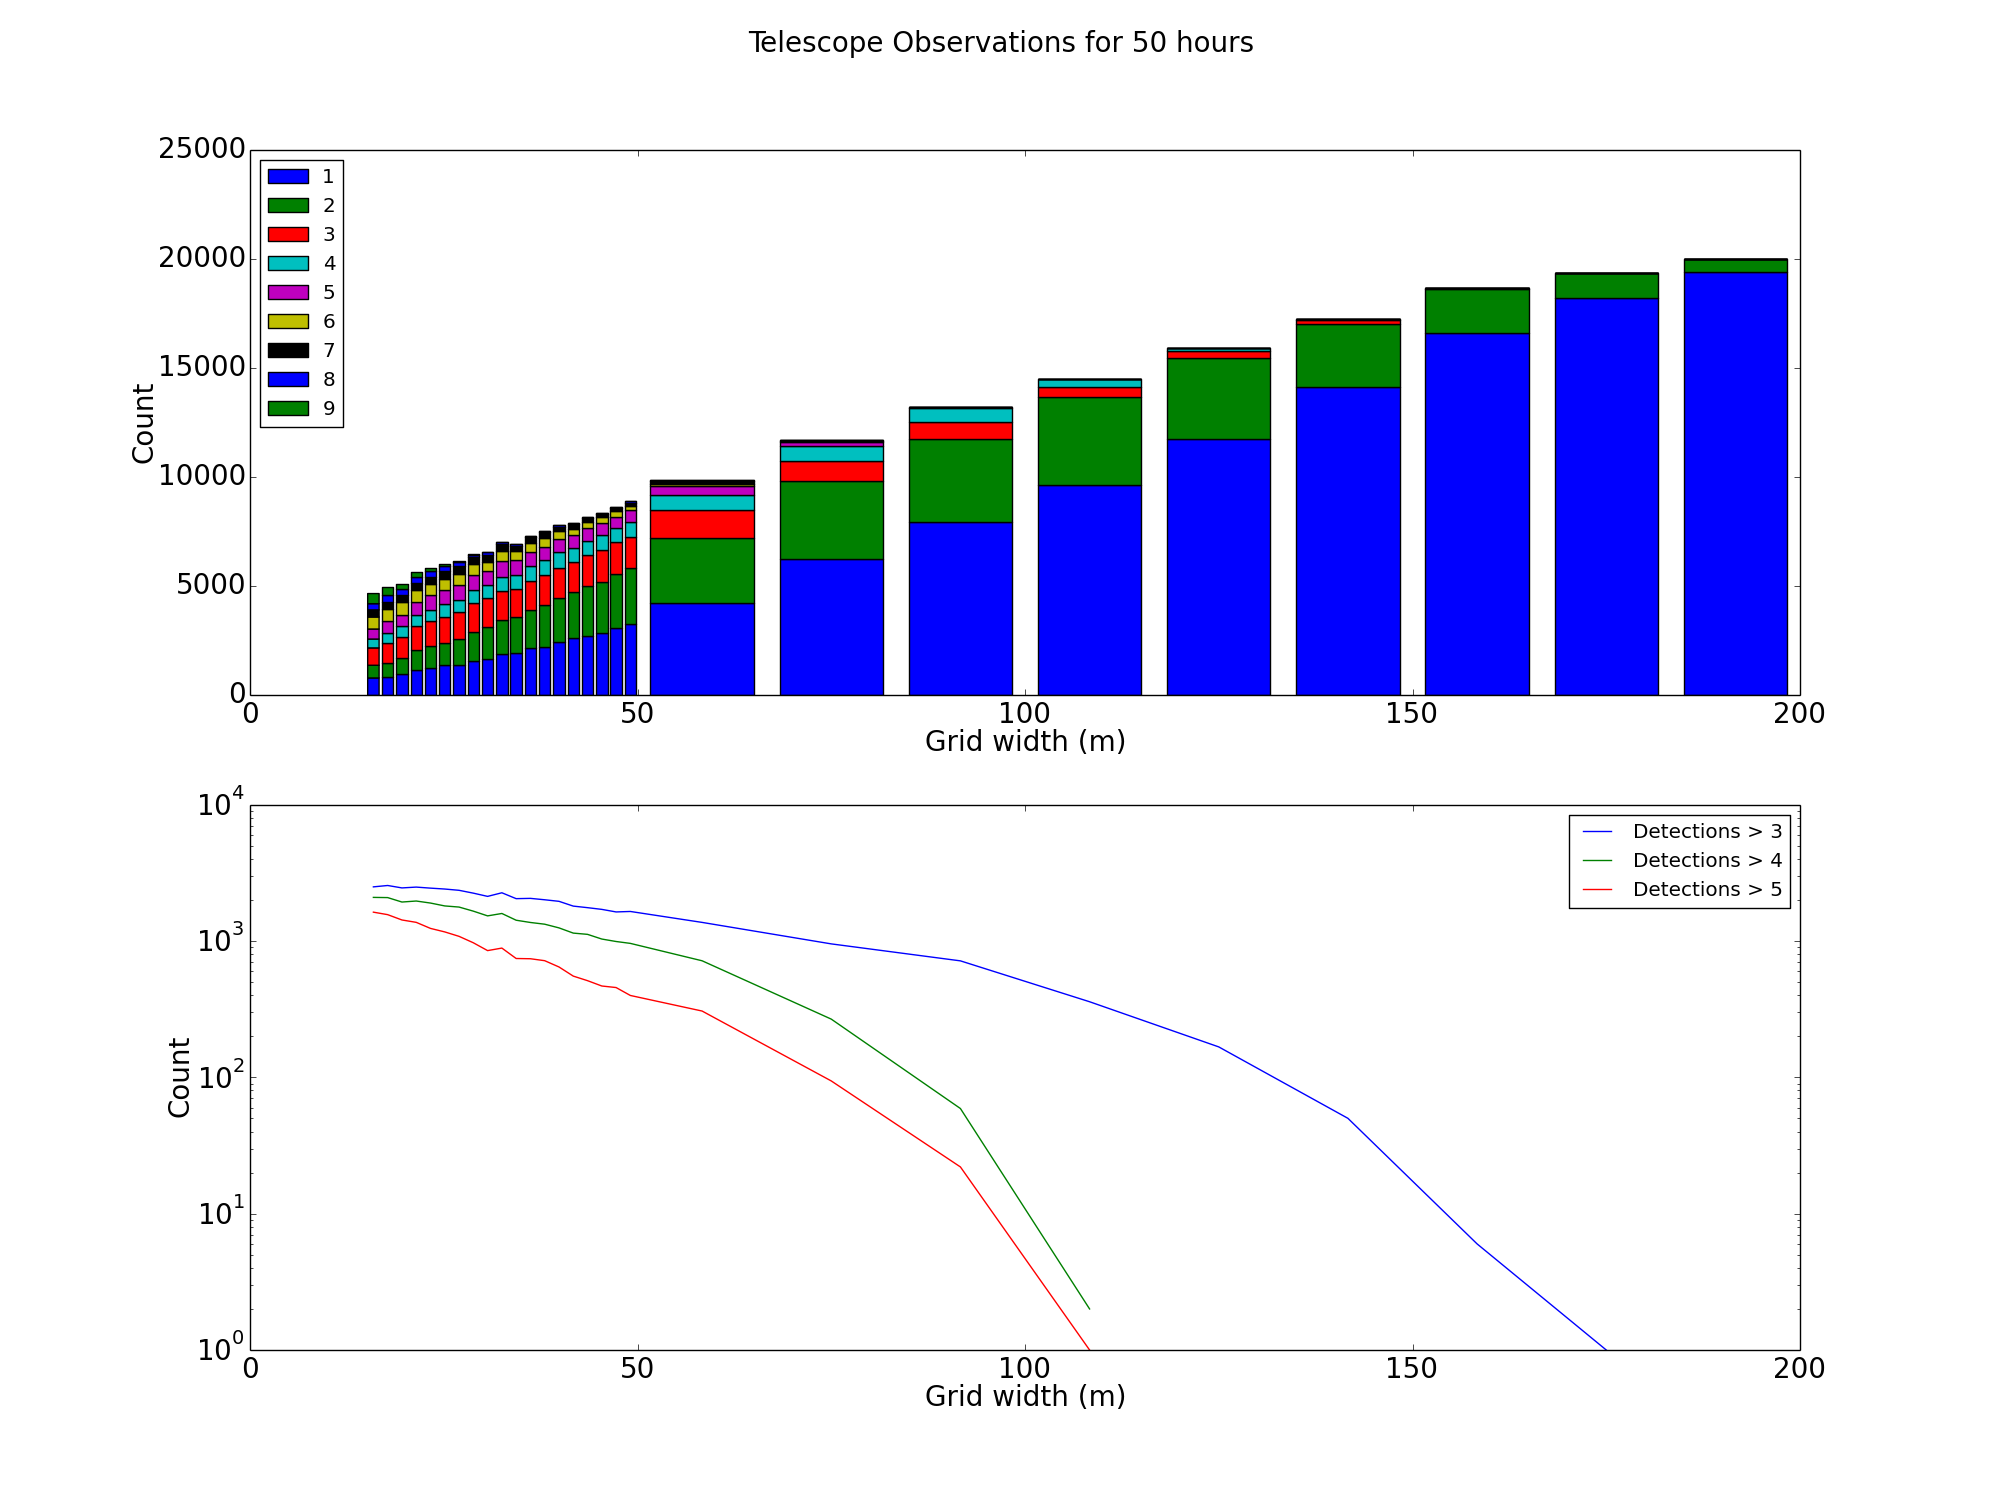
\includegraphics[width=0.9\textwidth]{optimiselayout}
\caption{A simulation of 50 hours of run time for various grid spacing for a 3x3 telescope array. Although raw count rate increases with increasing grid width, the \textquoteleft good count' rate of events observed by sufficient telescopes falls rapidly with increasing grid width}
\label{fig:optmiselayout}
\end{center}
\end{figure}

\section{Conclusion}
Preliminary results suggest that the LPD reconstruction technique will significantly improve charge reconstruction, to a level sufficient for cosmic ray abundance studies. However, reliance on high-multiplicity events means that although applicable to current experiments such as HESS, a new optimised telescope array would be required for a statistical analysis. Such an array may have a grid spacing of 20-50m, although further study is needed to determine the ideal layout.

The stated aim of this study was the Reconstruction of Charge Number of Heavy Cosmic Rays using Cherenkov Light. Broken down further, this analysis aimed to identify DC pixels in camera Images, to make a measurement of the DC light, and to reconstruct the charge of the Cosmic Ray with an error or roughly $\sigma_{Z}=1$ or less. On all of these counts, it is fair to say that the project was successful.

On the first count, the use of BDTs was overwhelmingly successful for identifying DC pixels. On a single Image basis, the BDT method produced an eightfold increase in accepted pixels with an accompanying decrease in the proportion of misidentified pixels. More importantly, the BDTs produced a two-hundred-fold increase in the acceptance of high-multiplicity events upon which this analysis depends. Combining the acceptance rates, we find that 2.3\% of all Iron Cosmic Rays with an Energy greater than 35 TeV will belong to a high-multiplicity image set. This gives an expected high-multiplicity Iron event rate of $1.22 \, h^{-1}$, rather than the alternative rate of $6.1 \times 10 ^{-3} \, h^{-1}= 1.02 \, week^{-1}$ that we would achieve with traditional $Q_{DC}$ identification. Ultimately, any attempted to analyse experimental data will suffer from vastly insufficient statistics unless the BDT method is applied for DC pixels. This technique will have wide-ranging uses outside of this analysis, among these will hopefully be a significant improvement in Hillas reconstruction. 

The second goal was achieved through use of a second set of BDTs, in this case regressors, to extract values for $DC_{rgr}$ from images using DC pixels. It was found that the actual quantity of DC light $True_{DC}$ varied quite significantly with the first interaction height. The time required to produce the five simulations seen in Figure \ref{fig:lpd} was approximately two minutes, and we might thus expect a calculation involving a thoroughly simulated LPD to last 10-20 seconds. The exact calculation time would be energy dependent. If we were to fully simulate the LPD for each iteration of the LPD, in order to realistically simulate the interaction height dependence,  we can see how long we might expect a minimisation of several thousand iterations to take. Each minimisation is itself only one of several hundred, making clear that such  fully simulating the LPD as part of a minimisation process is completely infeasible. 

Our only viable alternative is to develop a technique for measuring $True_{DC}$ without fully simulating the entire LPD. Fortunately, the BDT regressor was able to  do exactly this. The fractional standard deviation was reduced of the BDT was just $\frac{\sigma_{rgr}}{DC_{rgr}} = 0.14$ for a sample of mixed interaction heights, as opposed to $\frac{\sigma_{TrueDC}}{True_{DC}} = 0.48$ when the actual DC light was measured. With 4 or 5 LPD measurements, this BDT regressor was capable of giving an amplitude proportional to $Z^{2}$ with sufficient precision to enable reconstruction. The regressor was able to the necessary precision by correlating a number of image and pixel variables such as the Image Amplitude and Aspect Ratio. The BDT must indirectly be inferring the charge number, but by providing this information in the form of an LPD rather than a simple number, we are able to reconstruct the charge using all available information. It would be interesting to explore the possibility of a BDT that would directly calculate the charge number of a Cosmic Ray based on a given image, but this was not done as part of this analysis.

Our last goal was to reconstruct the charge number of Cosmic Rays. To be more specific, the reconstructed charge number should have a reasonably good resolution, while still having a reasonably high acceptance rate that means a spectroscopic analysis of heavy Cosmic Rays would be possible. Through a combination of two well-defined LPDs, it was possible to reconstruct events using a likelihood minimisation. This resulted in many high-multiplicity events, but the vast majority were 4-tel events with a charge resolution of $\sigma_{Z} = 2.2$. However, a third BDT was again able to significantly improve these results. In particular, 4-tel events were very easy to separate on the basis of their reconstructed energy and core position into groups of \textquoteleft Good' and \textquoteleft Bad' reconstructions. Using only those events which were deemed by the BDT to probably be well reconstructed, we noticeably reduce the charge resolution. Ultimately we are left with $\sigma_{Z}=1.05$ and $\sigma_{Z}=0.87$ for 4-tel and 5-tel events respectively. The resolutions, alongside the pass rate of 0.54 and 0.96, should be good enough to allow measurement of Cosmic Ray composition.

Having successfully reconstructed a relatively large and narrow Iron peak, it is safe to say that this analysis was a clear proof of concept. It remains to be seen whether the technique can be applied to real HESS data so effectively as the simulations suggest, but there is sufficient evidence to be optimistic. At the very least, the use of BDTs have provided significant improvements in the viability of LPD-based reconstruction.
\newpage
\section{Acknowledgements}
I would firstly like to thank Professor Dieter Horns, who served as a supervisor without flaw. I would particularly like to thank him for encouraging  me to present part of this work at a conference, as well as for occasionally providing Ice Cream to group members in the summer. Both were highly appreciated. 

In addition, I would like to thank Attila Abramowski for our many discussions about the HESS experiment and DC light. He was patient enough share his experience, which often served as a much-needed sanity check on my results. 

More generally, I would like to thank every member of the group, all of whom invariably made me feel welcome. I've really enjoyed my time as part of this group and they were the reason why. I feel luckily to have found a research group full of such genuinely nice people. (Apologies for Brexit!)
\newpage
\section{Bibliography}
\bibliographystyle{unsrt}
\bibliography{report}
\section{Appendix}
\subsection{Atmospheric Data Table for CORSIKA (Windhoek, Namibia)}
\begin{center}
\begin{small}
\setstretch{1.0}
\pgfplotstabletypeset{data/atmprof10.dat}
\end{small}
\end{center}
\end{document}